\def\printmanual{true}
% arara: makeindex

% Template for IEEE papers
%% bare_conf.tex
%% V1.4b
%% 2015/08/26
%% by Michael Shell
%% See:
%% http://www.michaelshell.org/
%% for current contact information.
%%
%% This is a skeleton file demonstrating the use of IEEEtran.cls
%% (requires IEEEtran.cls version 1.8b or later) with an IEEE
%% conference paper.
%%
%% Support sites:
%% http://www.michaelshell.org/tex/ieeetran/
%% http://www.ctan.org/pkg/ieeetran
%% and
%% http://www.ieee.org/

%%*************************************************************************
%% Legal Notice:
%% This code is offered as-is without any warranty either expressed or
%% implied; without even the implied warranty of MERCHANTABILITY or
%% FITNESS FOR A PARTICULAR PURPOSE!
%% User assumes all risk.
%% In no event shall the IEEE or any contributor to this code be liable for
%% any damages or losses, including, but not limited to, incidental,
%% consequential, or any other damages, resulting from the use or misuse
%% of any information contained here.
%%
%% All comments are the opinions of their respective authors and are not
%% necessarily endorsed by the IEEE.
%%
%% This work is distributed under the LaTeX Project Public License (LPPL)
%% ( http://www.latex-project.org/ ) version 1.3, and may be freely used,
%% distributed and modified. A copy of the LPPL, version 1.3, is included
%% in the base LaTeX documentation of all distributions of LaTeX released
%% 2003/12/01 or later.
%% Retain all contribution notices and credits.
%% ** Modified files should be clearly indicated as such, including  **
%% ** renaming them and changing author support contact information. **
%%*************************************************************************


% *** Authors should verify (and, if needed, correct) their LaTeX system  ***
% *** with the testflow diagnostic prior to trusting their LaTeX platform ***
% *** with production work. The IEEE's font choices and paper sizes can   ***
% *** trigger bugs that do not appear when using other class files.       ***                          ***
% The testflow support page is at:
% http://www.michaelshell.org/tex/testflow/

\documentclass{book}
\usepackage[quiet]{fontspec}
\usepackage[table,xcdraw,dvipsnames]{xcolor} % Used by spritegrid and others.
\usepackage[obeyspaces,spaces]{url}
\usepackage{longtable}
\usepackage{arydshln}
\usepackage{booktabs}
\usepackage{afterpage}
\usepackage{flushend}
\usepackage{titletoc}
\usepackage[toc]{appendix}
\usepackage{parskip}
\usepackage{graphicx,wrapfig}
\usepackage{float}
\usepackage{caption}
\usepackage{pdfpages}
\usepackage{tikzpagenodes}
\usepackage{imakeidx}
\usepackage[pagestyles,raggedright]{titlesec}
\usepackage[all]{nowidow}
\usepackage[bookmarks=true,linktoc=all]{hyperref}
\usepackage{tabularx}
\hypersetup{
  colorlinks   = true, %Colours links instead of ugly boxes
  urlcolor     = blue, %Colour for external hyperlinks
  % Each main .tex file configures via \titleformat the \chapter command
  % to do {\chapmtoc\insertminitoc} and \chapmtoc, as defined below, will
  % use \hypersetup{linkcolor=white} to avoid blue-on-blue TOC links
  % Besides, each main .tex file will issue the \tableofcontents command
  % between \hypersetup{linkcolor=black} and \hypersetup{linkcolor=blue}
  % This means however that if "blue" is modified here it must be modified
  % in these files too.
  linkcolor    = blue, %Colour of internal links
  citecolor   = red %Colour of citations
}
\usepackage{aeb-minitoc}
\usepackage{fix-cm}
\usepackage{textpos}
\usepackage{enumitem}
\usepackage{tcolorbox}
\tcbuselibrary{breakable,listings,skins,xparse}
%\usepackage{wrapfig}
\usepackage{needspace}
\usepackage{verbatim}
\usepackage{ean13isbn}
\usepackage{setspace}

% Use CHAPTER-PAGE page numbering to make it easier to modify chapters
% later, without messing up page number of the rest of the book.
\usepackage[auto]{chappg}

% Allow cross-references between the various books to the big The MEGA65 Book
\usepackage{xr}
\usepackage{varioref}
\usepackage{xparse}

\usepackage{colortbl}
\usepackage{adjustbox}

\externaldocument[M65Book-]{mega65-book}
% And a \ref alternative that checks if it needs to be a cross-reference to the
% MEGA65 Book instead.
\makeatletter
\newcommand{\bookref}[1]{%
    \@ifundefined{r@#1}{%
      {\em the MEGA65 Book}, \nameref{M65Book-#1} (\autoref{M65Book-#1})}{\autoref{#1}}%
}
\newcommand{\bookvref}[1]{%
    \@ifundefined{r@#1}{%
      {\em the MEGA65 Book}, \nameref{M65Book-#1} (\autoref{M65Book-#1})}{Chapter/Appendix \vref{#1}}%
}
\makeatother

% For fixed-width columns in register maps
\usepackage{array}

% Makes tables with double-ruled lines look better
\usepackage{hhline}

% Makes better use of space for reference tables in appendix
\usepackage{multicol}

% Shaded tables with alternate rows colored for better legibility
% Best used with larger tables rather than small tables
\usepackage{colortbl}
\usepackage{adjustbox}
\usepackage[strict]{changepage}

% \makecell command for forcing line breaks in table cells
\usepackage{makecell}

\newcolumntype{L}[1]{>{\raggedright\let\newline\\\arraybackslash\hspace{0pt}}m{#1}}
\newcolumntype{C}[1]{>{\centering\let\newline\\\arraybackslash\hspace{0pt}}m{#1}}
\newcolumntype{R}[1]{>{\raggedleft\let\newline\\\arraybackslash\hspace{0pt}}m{#1}}

% clear to left page for making two page tables starting on the odd page
\newcommand{\cleartoleftpage}{%
  \clearpage
  \ifodd\value{page}\hbox{}\newpage\fi
}

% Layout structures for acknowledgements pages
\newenvironment{mega65thanks}{
    \setlength{\linewidth}{125mm}
    \setlength{\columnsep}{3mm}
    \begin{multicols}{2}
}{
    \end{multicols}
}


% For displaying Letter keys and the MEGA key
% This is a `keys' element for displaying a Mega65 keyboard key
% using a black filled label with rounded edges.
% In order to display a key as a title, use:
%
%     \megakey[title]{Run/Stop}
%
% For displaying a key as a part of the normal document flow, simply use:
%
%    \megakey{Shift}
% 
% Other sizes are supported, as part of tcolorbox: http://mirror.aarnet.edu.au/pub/CTAN/macros/latex/contrib/tcolorbox/tcolorbox.pdf#subsubsection.4.7.5 however, only `title' and the default: `small' are proposed for use in this manual.

\usepackage{tcolorbox}
\usepackage[utf8]{inputenc}

\newtcbox{\megakey}[1][small]{colback=black, coltext=white, size=#1, fontupper=\bfseries\uppercase,nobeforeafter,box align=bottom,text height=7pt}


% For displaying print versions petscii character symbols
% This is a collection of symbol macros element for displaying a printed version of the
% MEGA65 graphic characters, as opposed to the bitmap versions in the mega40/80.ttf fonts files.
% You can display characters using the graphicsymbol macro:
%
%    \graphicsymbol{\textcolor{red}{qQ} wWUcbdhjI \textcolor{blue}{JK}}
%
% Or you can, simply use the font itself:
%
%    \begin{symbolfont}%
%	   qQwWeErRtTyYuUiIoOpP\\
%		 aAsSdDfFgGhHjJkKlL\\
%		 zZxXcCvVbBnNmM%
%		 \end{symbolfont}%
%
%
% You can display the MEGA symbol using:
%
%    \megasymbol
%
% This will display the symbol in black. Other colours can be specified by passing them in, for example:
%
% 	 \megasymbol[black]
%		 \megasymbol[white]
%		 \megasymbol[orange]
%		 \megasymbol[blue]
%
% NOTE:
% For using the MEGA symbol in a key, see the \megasymbolkey macro in the keys.txt file.

\usepackage{tcolorbox}

\newcommand{\graphicsymbol}[1]{\begin{symbolfont}#1\end{symbolfont}}

\newcommand{\megasymbol}[1][black]{\begin{symbolfont}\textcolor{#1}{`}\end{symbolfont}}


% For Mega65 display of code, listings and screen activity
% This is a collection of elements for displaying output from the Mega65 screen.
% They can display program code or fragments to show activity on the screen.
% Example of use:
%
%    \begin{screenoutput}
%    10 OPEN 1,8,0,"$0:*,P,R
%    20 : IF DS THEN PRINT DS$: GOTO 100
%    30 GET#1,X$,X$
%    40 DO
%    50 : GET#1,X$,X$: IF ST THEN EXIT
%    60 : GET#1,BL$,BH$
%    70 : LINE INPUT#1, F$
%    80 : PRINT LEFT$(F$,18)
%    90 LOOP
%    100 CLOSE 1
%
%    RUN
%    \end{screenoutput}
%
% for inline display of code, use:
%
%    \screentext{?SYNTAX ERROR}
%

\usepackage{listings,color}

\lstnewenvironment{screenoutput}
   {
     \lstset{
               basicstyle=\codefont\color{white}\linespread{1.0}\normalsize,
               backgroundcolor=\color{black},fillcolor=\color{black},
               rulecolor=\color{black},
               frame=lines,
               framexleftmargin=2mm,
               framexrightmargin=2mm,
               framextopmargin=2mm,
               framexbottommargin=2mm,
               tabsize=4,
               xleftmargin=2mm,
               xrightmargin=2mm,
               basewidth={0.4em},
               literate={\*}{*}1{\-}{-}1{\/}{/}1{{\ }}{{ }}1
            }
   }
   {  }


% For in-line screen text
\newcommand{\screentext}[1]{ {\codefont\color{black}\normalsize{#1}} }


% For MEGA65 screen shots with text flow
\newcommand{\screenshotwrap}[1]{{\begin{center}\includegraphics[width=0.80\linewidth]{#1}\end{center}}}
%\newcommand{\screenshotwrap}[1]{\needspace{8cm}\setlength{\intextsep}{0pt}\begin{wrapfigure}{i}{0.80\textwidth}\includegraphics[width=\linewidth]{#1}\end{wrapfigure}}


% For displaying sprite data in a grid
% This is an element for displaying a sprite in a grid, just like page 70 of the
% commodore manual. This version can be easily expanded. For now it will suffice.
% In order to display a hi-res mono sprite grid use:
%
%	\spritegrid{
%	\hline
%	\spritecells{---------ooooooo--------}
%	\spritecells{-------ooooooooooo------}
%	\spritecells{------ooooooooooooo-----}
%	\spritecells{------ooooo--oooooo-----}
%	\spritecells{-----ooooo-oo--ooooo----}
%	\spritecells{-----ooooo-ooooooooo----}
%	\spritecells{-----ooooo-oo--ooooo----}
%	\spritecells{------ooooo--oooooo-----}
%	\spritecells{------ooooooooooooo-----}
%	\spritecells{------ooooooooooooo-----}
%	\spritecells{------o-ooooooooo-o-----}
%	\spritecells{-------o-ooooooo-o------}
%	\spritecells{-------o--ooooo--o------}
%	\spritecells{--------o--ooo--o-------}
%	\spritecells{--------o--ooo--o-------}
%	\spritecells{---------o--o--o--------}
%	\spritecells{---------o--o--o--------}
%	\spritecells{----------ooooo---------}
%	\spritecells{----------ooooo---------}
%	\spritecells{----------ooooo---------}
%	\spritecells{-----------ooo----------}
%	}
%
% For a multicolour sprite:
%
%	\spritegrid{
%	\hline
%	\spritecells{------------------------}
%	\spritecells{------------------------}
%	\spritecells{------------------------}
%	\spritecells{------------------------}
%	\spritecells{--------llllll----------}
%	\spritecells{------llllllggll--------}
%	\spritecells{------llllllllgg--------}
%	\spritecells{----llllllgggggggg------}
%	\spritecells{----llllggeeeellll------}
%	\spritecells{----lloollllllggee------}
%	\spritecells{----llooggggooggee------}
%	\spritecells{----llooggggooggee------}
%	\spritecells{----eeeeggggooeeee------}
%	\spritecells{----ggeeeeeeeeoo--------}
%	\spritecells{------ggooooooee--------}
%	\spritecells{------eeggeeeeee--------}
%	\spritecells{--------eeeeee----------}
%	\spritecells{------------------------}
%	\spritecells{------------------------}
%	\spritecells{------------------------}
%	\spritecells{------------------------}
%	}

\usepackage{tabulary} %Removes spacing from tabulars
\usepackage{xstring} % for string substitution
\usepackage{xparse} % used for unpacking the sprite characters
% \renewcommand{\familydefault}{\sfdefault} % default sans font

%\usepackage{graphicx} % for resizing the tabular used by spritegrid
\usepackage{subcaption} % used for the left hand subtable of row numbers
\usepackage{multirow} % used for the ``Row'' column
\usepackage{rotating} % used by the rotating ``Row'' word

\newcommand{\spritebytecolumn}[1]{
   %\framebox[4mm]{#1}
   \makebox[4mm]{#1}
}

\setlength\tabcolsep{0.3mm} % the indivdual cell width and height

% The byte numbers at the top of the grid in two jaged rows. 
\newcommand{\spritetopcolumnbytenumbers}{
  \spritebytecolumn{128} & 
  \spritebytecolumn{ } & 
  \spritebytecolumn{32} & 
  \spritebytecolumn{ } &

  \spritebytecolumn{8} & 
  \spritebytecolumn{ } & 
  \spritebytecolumn{2} & 
  \spritebytecolumn{} %\\[-2pt]
}

\newcommand{\spritebottomcolumnbytenumbers}{
  \spritebytecolumn{ } & 
  \spritebytecolumn{64} & 
  \spritebytecolumn{ } & 
  \spritebytecolumn{16} &
  
  \spritebytecolumn{ } & 
  \spritebytecolumn{4} & 
  \spritebytecolumn{ } & 
  \spritebytecolumn{1} 
}


% Cell colour list. Can be expanded for other colours in the sprite grid
\def\blk{\cellcolor{black}}
\def\wht{\cellcolor{white}}
\def\grn{\cellcolor{ForestGreen}}
\def\lgrn{\cellcolor{YellowGreen}}
\def\gry{\cellcolor{Gray}}

\newcounter{lettercounter} % counter for detecting the last cell

% Collect the spritecell list and send it to \ProcessSpriteCell for turning into cells
\NewDocumentCommand{\spritecells}{%
>{\SplitList{}} m }{%
  \ProcessList{#1}{\ProcessSpriteCell}%
}

\NewDocumentCommand{\ProcessSpriteCell}{m}{%
  \stepcounter{lettercounter}% 
    \IfStrEqCase{#1}{
	{o}{\blk}
	{-}{\wht}
	{g}{\grn}
	{l}{\lgrn}
	{e}{\gry}
   }%
   \IfStrEq{\thelettercounter}{24}{\setcounter{lettercounter}{0} \\ \hline}{&}%
}

% Start of the actual spritegrid definition
\newcommand{\spritegrid}[1]{
\begin{table}[h!]
\centering
\begin{subtable}{28mm}
\vspace{8mm}
\scalebox{0.76}{
\begin{tabular}{p{25mm} p{4mm} c}
\multirow{21}{*}{ } &
\multirow{21}{*}{%
\begin{turn}{90}%
\bfseries\uppercase{Row}%
\end{turn}} &
 1\\
& & 2\\
& & 3\\
& & 4\\
& & 5\\
& & 6\\
& & 7\\
& & 8\\
& & 9\\
& & 10\\
& & 11\\
& & 12\\
& & 13\\
& & 14\\
& & 15\\
& & 16\\
& & 17\\
& & 18\\
& & 19\\
& & 20\\
& & 21
\end{tabular}
}
\end{subtable}%
\begin{subtable}{.8\textwidth}

\setlength{\arrayrulewidth}{1pt}
\scalebox{0.7}{%
\begin{tabular}{  *{3}{p{30mm} }  }
  \center\uppercase{Series\\1} &
  \center\uppercase{Series\\2} &
  \center\uppercase{Series\\3}  
\end{tabular}%
}

\scalebox{0.7}{
\begin{tabular}{  *{24}{p{3.35mm} }  }
	\spritetopcolumnbytenumbers & 
	\spritetopcolumnbytenumbers & 
	\spritetopcolumnbytenumbers \\
	\spritebottomcolumnbytenumbers &
	\spritebottomcolumnbytenumbers &
	\spritebottomcolumnbytenumbers
\end{tabular} 
}

\scalebox{0.7}{
\begin{tabular}{ | *{24}{p{3mm} |}  }
#1
\end{tabular}
}

\scalebox{0.7}{
\begin{tabular}{ *{24}{p{3.35mm}}  }
	\spritebytecolumn{1} & & & & 
	\spritebytecolumn{5} & & & & & 
	\spritebytecolumn{10} & & & & & 
	\spritebytecolumn{15} & & & & & 
	\spritebytecolumn{20} & & & & 
	\spritebytecolumn{24} \\
	\multicolumn{24}{c}{\bfseries\uppercase{Column}}
\end{tabular}
}
\end{subtable}
\end{table}
}

% End of the actual spritegrid definition

% Don't number sections
\setcounter{secnumdepth}{0}

\renewcommand{\indexname}{INDEX}
\renewcommand{\appendixtocname}{APPENDICES}
\renewcommand{\appendixpagename}{APPENDICES}
\renewcommand{\appendixpage}{%
  \clearpage\thispagestyle{empty}
    \pagecolor{blue}
     \begin{center}
       {
         \large
         % Put a nice amount of vertical space before the title
         \vspace*{2cm}
               {\large\Huge\textcolor{white}{\bf{APPENDICES}}}\\
             \vspace{\fill}
       }
     \end{center}
     \newpage\pagecolor{white}\clearpage
}

\makeatletter\chardef\pdf@shellescape=\@ne\makeatother

\setcounter{tocdepth}{5}

% 1.0 cm is the distance from left of page to bullet point.
% 2.8 cm is a fudge-factor to make multi-line section names be correctly lined up.
% \@B{〈length〉} is the amount to indent prior to〈sec-num >
% \@F{〈fmt〉} is the formatting for the title heading
% \@P{〈fmt〉} is the formatting for the page number (〈pg-num〉).

\TOCLevels{chapter}{section}
\begin{minitocfmt}{\chapmtoc}
\declaretocfmt{section}{\@F{\color{white}\hypersetup{linkcolor=white}\hspace{1.0cm}\textbullet\hspace{0.25cm}\Large\bfseries}\@B{2.8cm}\@P{\mtocgobble}}
\declaretocfmt{section*}{\@F{\color{white}\hypersetup{linkcolor=white}\hspace{1.0cm}\textbullet\hspace{0.25cm}\Large\bfseries}\@B{2.8cm}\@P{\mtocgobble}}
\end{minitocfmt}

\usepackage{fontspec}

\setmainfont[Path=fonts/, BoldFont=GlacialIndifference-Bold.otf, ItalicFont=GlacialIndifference-Italic.otf]{GlacialIndifference-Regular.otf}
\newfontfamily\serifed[Path=fonts/, BoldFont=xits-bold.otf, ItalicFont=xits-italic.otf]{xits-regular.otf}
\newfontface\codefont[Path=fonts/]{mega80.ttf}
\newfontface\symbolfont[Path=fonts/]{MEGA65GraphicSymbols.otf}


% Set margins for inner and outer pages in A5 book format
\ifdefined\printmanual
\usepackage[a5paper,nomarginpar,includemp,bottom=2cm,top=1cm,inner=1.8cm,outer=0.8cm, footskip = 1cm]{geometry}
\else
\usepackage[a5paper,nomarginpar,includemp,bottom=2cm,top=1cm,inner=1.0cm,outer=1.0cm, footskip = 1cm]{geometry}
\fi

% Some Computer Society conferences also require the compsoc mode option,
% but others use the standard conference format.
%
% If IEEEtran.cls has not been installed into the LaTeX system files,
% manually specify the path to it like:
% \documentclass[conference]{../sty/IEEEtran}

%% % Some very useful LaTeX packages include:

% *** MISC UTILITY PACKAGES ***
%
%\usepackage{ifpdf}
% Heiko Oberdiek's ifpdf.sty is very useful if you need conditional
% compilation based on whether the output is pdf or dvi.
% usage:
% \ifpdf
%   % pdf code
% \else
%   % dvi code
% \fi
% The latest version of ifpdf.sty can be obtained from:
% http://www.ctan.org/pkg/ifpdf
% Also, note that IEEEtran.cls V1.7 and later provides a builtin
% \ifCLASSINFOpdf conditional that works the same way.
% When switching from latex to pdflatex and vice-versa, the compiler may
% have to be run twice to clear warning/error messages.



\usepackage{csquotes}


% *** CITATION PACKAGES ***
%
\usepackage{cite}
% cite.sty was written by Donald Arseneau
% V1.6 and later of IEEEtran pre-defines the format of the cite.sty package
% \cite{} output to follow that of the IEEE. Loading the cite package will
% result in citation numbers being automatically sorted and properly
% "compressed/ranged". e.g., [1], [9], [2], [7], [5], [6] without using
% cite.sty will become [1], [2], [5]--[7], [9] using cite.sty. cite.sty's
% \cite will automatically add leading space, if needed. Use cite.sty's
% noadjust option (cite.sty V3.8 and later) if you want to turn this off
% such as if a citation ever needs to be enclosed in parenthesis.
% cite.sty is already installed on most LaTeX systems. Be sure and use
% version 5.0 (2009-03-20) and later if using hyperref.sty.
% The latest version can be obtained at:
% http://www.ctan.org/pkg/cite
% The documentation is contained in the cite.sty file itself.






% *** GRAPHICS RELATED PACKAGES ***
%
\ifCLASSINFOpdf
   \usepackage[pdftex]{graphicx}
  % declare the path(s) where your graphic files are
   \graphicspath{{../pdf/}{../jpeg/}}
  % and their extensions so you won't have to specify these with
  % every instance of \includegraphics
   \DeclareGraphicsExtensions{.pdf,.jpeg,.png}
\else
  % or other class option (dvipsone, dvipdf, if not using dvips). graphicx
  % will default to the driver specified in the system graphics.cfg if no
  % driver is specified.
   \usepackage[dvips]{graphicx}
  % declare the path(s) where your graphic files are
%   \graphicspath{{../eps/}}
  % and their extensions so you won't have to specify these with
  % every instance of \includegraphics
   \DeclareGraphicsExtensions{.eps}
\fi
% graphicx was written by David Carlisle and Sebastian Rahtz. It is
% required if you want graphics, photos, etc. graphicx.sty is already
% installed on most LaTeX systems. The latest version and documentation
% can be obtained at: 
% http://www.ctan.org/pkg/graphicx
% Another good source of documentation is "Using Imported Graphics in
% LaTeX2e" by Keith Reckdahl which can be found at:
% http://www.ctan.org/pkg/epslatex
%
% latex, and pdflatex in dvi mode, support graphics in encapsulated
% postscript (.eps) format. pdflatex in pdf mode supports graphics
% in .pdf, .jpeg, .png and .mps (metapost) formats. Users should ensure
% that all non-photo figures use a vector format (.eps, .pdf, .mps) and
% not a bitmapped formats (.jpeg, .png). The IEEE frowns on bitmapped formats
% which can result in "jaggedy"/blurry rendering of lines and letters as
% well as large increases in file sizes.
%
% You can find documentation about the pdfTeX application at:
% http://www.tug.org/applications/pdftex





% *** MATH PACKAGES ***
%
%\usepackage{amsmath}
% A popular package from the American Mathematical Society that provides
% many useful and powerful commands for dealing with mathematics.
%
% Note that the amsmath package sets \interdisplaylinepenalty to 10000
% thus preventing page breaks from occurring within multiline equations. Use:
%\interdisplaylinepenalty=2500
% after loading amsmath to restore such page breaks as IEEEtran.cls normally
% does. amsmath.sty is already installed on most LaTeX systems. The latest
% version and documentation can be obtained at:
% http://www.ctan.org/pkg/amsmath





% *** SPECIALIZED LIST PACKAGES ***
%
%\usepackage{algorithmic}
% algorithmic.sty was written by Peter Williams and Rogerio Brito.
% This package provides an algorithmic environment fo describing algorithms.
% You can use the algorithmic environment in-text or within a figure
% environment to provide for a floating algorithm. Do NOT use the algorithm
% floating environment provided by algorithm.sty (by the same authors) or
% algorithm2e.sty (by Christophe Fiorio) as the IEEE does not use dedicated
% algorithm float types and packages that provide these will not provide
% correct IEEE style captions. The latest version and documentation of
% algorithmic.sty can be obtained at:
% http://www.ctan.org/pkg/algorithms
% Also of interest may be the (relatively newer and more customizable)
% algorithmicx.sty package by Szasz Janos:
% http://www.ctan.org/pkg/algorithmicx




% *** ALIGNMENT PACKAGES ***
%
%\usepackage{array}
% Frank Mittelbach's and David Carlisle's array.sty patches and improves
% the standard LaTeX2e array and tabular environments to provide better
% appearance and additional user controls. As the default LaTeX2e table
% generation code is lacking to the point of almost being broken with
% respect to the quality of the end results, all users are strongly
% advised to use an enhanced (at the very least that provided by array.sty)
% set of table tools. array.sty is already installed on most systems. The
% latest version and documentation can be obtained at:
% http://www.ctan.org/pkg/array


% IEEEtran contains the IEEEeqnarray family of commands that can be used to
% generate multiline equations as well as matrices, tables, etc., of high
% quality.

%%%%%%%%%%%%%%%%%
\usepackage{multirow}
\usepackage[table]{xcolor}
\usepackage{tablefootnote}
\usepackage[bottom]{footmisc}

%%%%%%%%%%%%%%%%%%

% *** SUBFIGURE PACKAGES ***
\ifCLASSOPTIONcompsoc
  \usepackage[caption=false,font=normalsize,labelfont=sf,textfont=sf]{subfig}
\else
  \usepackage[caption=false,font=footnotesize]{subfig}
\fi
% subfig.sty, written by Steven Douglas Cochran, is the modern replacement
% for subfigure.sty, the latter of which is no longer maintained and is
% incompatible with some LaTeX packages including fixltx2e. However,
% subfig.sty requires and automatically loads Axel Sommerfeldt's caption.sty
% which will override IEEEtran.cls' handling of captions and this will result
% in non-IEEE style figure/table captions. To prevent this problem, be sure
% and invoke subfig.sty's "caption=false" package option (available since
% subfig.sty version 1.3, 2005/06/28) as this is will preserve IEEEtran.cls
% handling of captions.
% Note that the Computer Society format requires a larger sans serif font
% than the serif footnote size font used in traditional IEEE formatting
% and thus the need to invoke different subfig.sty package options depending
% on whether compsoc mode has been enabled.
%
% The latest version and documentation of subfig.sty can be obtained at:
% http://www.ctan.org/pkg/subfig




% *** FLOAT PACKAGES ***
%
%\usepackage{fixltx2e}
% fixltx2e, the successor to the earlier fix2col.sty, was written by
% Frank Mittelbach and David Carlisle. This package corrects a few problems
% in the LaTeX2e kernel, the most notable of which is that in current
% LaTeX2e releases, the ordering of single and double column floats is not
% guaranteed to be preserved. Thus, an unpatched LaTeX2e can allow a
% single column figure to be placed prior to an earlier double column
% figure.
% Be aware that LaTeX2e kernels dated 2015 and later have fixltx2e.sty's
% corrections already built into the system in which case a warning will
% be issued if an attempt is made to load fixltx2e.sty as it is no longer
% needed.
% The latest version and documentation can be found at:
% http://www.ctan.org/pkg/fixltx2e


%\usepackage{stfloats}
% stfloats.sty was written by Sigitas Tolusis. This package gives LaTeX2e
% the ability to do double column floats at the bottom of the page as well
% as the top. (e.g., "\begin{figure*}[!b]" is not normally possible in
% LaTeX2e). It also provides a command:
%\fnbelowfloat
% to enable the placement of footnotes below bottom floats (the standard
% LaTeX2e kernel puts them above bottom floats). This is an invasive package
% which rewrites many portions of the LaTeX2e float routines. It may not work
% with other packages that modify the LaTeX2e float routines. The latest
% version and documentation can be obtained at:
% http://www.ctan.org/pkg/stfloats
% Do not use the stfloats baselinefloat ability as the IEEE does not allow
% \baselineskip to stretch. Authors submitting work to the IEEE should note
% that the IEEE rarely uses double column equations and that authors should try
% to avoid such use. Do not be tempted to use the cuted.sty or midfloat.sty
% packages (also by Sigitas Tolusis) as the IEEE does not format its papers in
% such ways.
% Do not attempt to use stfloats with fixltx2e as they are incompatible.
% Instead, use Morten Hogholm'a dblfloatfix which combines the features
% of both fixltx2e and stfloats:
%
% \usepackage{dblfloatfix}
% The latest version can be found at:
% http://www.ctan.org/pkg/dblfloatfix


% *** PDF, URL AND HYPERLINK PACKAGES ***
%
\usepackage{url}
% url.sty was written by Donald Arseneau. It provides better support for
% handling and breaking URLs. url.sty is already installed on most LaTeX
% systems. The latest version and documentation can be obtained at:
% http://www.ctan.org/pkg/url
% Basically, \url{my_url_here}.


% *** Do not adjust lengths that control margins, column widths, etc. ***
% *** Do not use packages that alter fonts (such as pslatex).         ***
% There should be no need to do such things with IEEEtran.cls V1.6 and later.
% (Unless specifically asked to do so by the journal or conference you plan
% to submit to, of course. )


% *** Use glossaries for abbreviations ***
\usepackage[acronym, nowarn]{glossaries}
\makeglossaries
%!TEX root = pairing.tex
% ********************************************************************
% Definition of acronyms
% ********************************************************************
% Specify new acronyms using the following command:
% 	\newacronym{<label>}{<abbrv>}{<full>}
%
% Using acronyms in text is supported by using 
% 	\gls  	This command prints the term associated with <label>
% 	\glspr 	This command prints the plural of the defined term
% 	\Gls 	This command prints the singular form with the first character
%				converted to upper case.
% 	\Glspl Upercase, Plural

\newacronym{manet}{\textsc{MANET}}{mobile ad hoc networks}
\newacronym{tetra}{\textsc{TETRA}}{Terrestrial Trunked Radio}
\newacronym{hf}{\textsc{HF}}{High Frequency}
\newacronym{uhf}{\textsc{UHF}}{Ultra High Frequency}
\newacronym{vhf}{\textsc{VHF}}{Very High Frequency}
\newacronym{sbd}{\textsc{SBD}}{short-burst-data}

% *** Use SI Units
\usepackage[binary-units=true]{siunitx}
\sisetup{per-mode = symbol,
		 list-final-separator = {, and},
		 range-phrase = \ {;}\ ,
		 range-units  = brackets,
		 open-bracket = [,
	     close-bracket= ],}


% correct bad hyphenation here
\hyphenation{op-tical net-works semi-conduc-tor}

\makeindex[intoc]

\pagestyle{empty}

\begin{document}
\raggedbottom

% relax word wrapping with sloppy
\sloppy
% reduce overfull \hbox warnings
\hfuzz=5pt

% macro for changing the verbatim font
\makeatletter
\newcommand{\verbatimfont}[1]{\def\verbatim@font{#1}}%
\makeatother


%\pagecolor{blue}
%\clearpage\thispagestyle{empty}
%\begin{center}
%\includegraphics[width=\textwidth]{frontcover/MEGA65_logo_shadow}
%
%{\textcolor{white}{\large\Huge{\bf{USER'S GUIDE}}}}
%
%\vspace{\fill}
%\end{center}
%
\newcommand\titlestreq[3]{%
  \IfStrEq{#1}{\detokenize{#2}}{\includegraphics[height=210mm,width=149mm]{\detokenize{#3}}}{}%
}

\newcommand\titlepic[1]{%
  \titlestreq{#1}{mega65-book}{frontcover/m65book\_title}%
  \titlestreq{#1}{mega65-userguide}{frontcover/manual\_title}%
  \titlestreq{#1}{mega65-developer-guide}{frontcover/developer\_title}%
  \titlestreq{#1}{mega65-chipset-reference}{frontcover/chipset\_title}%
  \titlestreq{#1}{mega65-basic65-reference}{frontcover/basic65\_title}%
}

\begin{tikzpicture}[remember picture,overlay,shift={(current page.north east)}]
\node[anchor=north east,xshift=0.2cm,yshift=0.1cm]{\titlepic{\jobname}};
\end{tikzpicture}

%\newpage
%\pagecolor{white}

\chapter*{REGULATORY INFORMATION}

The MEGA65 home computer and portable computer have not been subject to FCC, EC
or other regulatory approvals as of the time of writing.

\chapter*{Reporting Errors and Omissions}

This book is being continuously refined and improved upon by the MEGA65 community.
The version of this edition is:

\input{gitinfo}

We want this book to be the best that it possibly can. So if you see any errors,
find anything that is missing, or would like more information,
please report them using the MEGA65 User's Guide issue tracker:

\url{https://github.com/mega65/mega65-user-guide/issues}

You can also check there to see if anyone else has reported a similar problem,
while you wait for this book to be updated.

Finally, you can always download the latest versions of our suite of books from these locations:

\begin{itemize}
\item \url{https://mega65.org/mega65-book}
\item \url{https://mega65.org/user-guide}
\item \url{https://mega65.org/developer-guide}
\item \url{https://mega65.org/basic65-ref}
\item \url{https://mega65.org/chipset-ref}
\item \url{https://files.mega65.org/manuals-upload}
\end{itemize}


\megabookstart{MEGA65 USER'S GUIDE}{2nd Edition}

\chapter{Introduction}

Congratulations on your purchase of one of the most long-awaited computers in the history of computing. The MEGA65 is a community designed computer, based on the never-released Commodore{\textregistered} 65\footnote{Commodore is a trademark of C= Holdings} computer; a computer designed in 1989 and intended for public release in 1990. Decades have passed, and the MEGA65 invokes an earlier time when computers were simple and friendly. They were not only simple to operate and understand how they work, but friendly and approachable for new users.

These 1980s computers inspired an entire generation of professionals to choose the exciting and rewarding technology careers they have today. Just imagine the joy of these individuals as they learned they could use their new computer to solve problems, write a letter, prepare taxes, invent new things, or even discover how the universe works. We want to re-create that level of excitement not found in modern computing, so we made the {\bf MEGA65}.

The MEGA65 team believes that owning a computer is like owning a home. You don't just use a home; you change things big and small to make it your own custom living space. After a while, when you settle in, you may decide to renovate or expand your home to make it more comfortable or provide more utility. Think of the MEGA65 as a "computing home".

This guide will teach you how to do more than just hang pictures on a wall, it will ask you to build your dream home. While you read this user's guide, you will learn how to operate the MEGA65, code programs, add additional software, and extend hardware capabilities. What won't be immediately obvious is that along the journey, you will also learn about the history of computing as you explore Commodore BASIC version 10 and operating system commands.

Computer graphics and music make computing more fun; and we designed the MEGA65 for fun! In this user's guide, you will learn to code using the MEGA65's built-in {\bf graphics} and {\bf sound} capabilities. But you don't need to be a coder to have fun with the MEGA65, as the MEGA65 includes a complete Commodore{\textregistered} 64{\texttrademark}\footnote{Commodore 64 is a trademark of C= Holdings, }, it can also run thousands of games, utilities, and business software from the past and new programs being written today by Commodore enthusiasts. Excitement for the MEGA65 will grow as we discover what programmers can do, as they learn about the power and features of this modern Commodore computer re-creation. Together, we will create a whole new "home-brew" community to do things that even we didn't think were possible when creating the MEGA65.

We welcome you on this journey! Thank you for becoming a part of the {\bf MEGA65}community of users, coders, and enthusiasts! Get involved, learn more about your MEGA65, and join us online at: \url{https://mega65.net}

% I thought a call to action to join the community would be good to add early on. Where will the final online community call home?

\section{Other Books in this series}

This is one of several MEGA65 documentation volumes.  The series includes:

\begin{itemize}
	\item The MEGA65 User Guide -- Provides an introduction to the MEGA65, and a condensed BASIC 10 command reference
	\item The MEGA65 BASIC 10 Reference Guide -- Comprehensive documentation of all BASIC 10 commands, functions and operators
	\item The MEGA65 Chipset Reference -- Detailed documentation about the MEGA65 and C65's custom chips
	\item The MEGA65 Developer Guide -- Information for developers wishing to write programmes for the MEGA65
	\item The MEGA65 Book -- All volumes in a single huge PDF for easy online searching. 850 pages and growing!
\end{itemize}


\cleardoublepage

\chapter{Setup}

\section{Unpacking and Connecting the MEGA65}
\label{cha:setup}

It is time to set up your MEGA65 home computer! The box contains the following:

\begin{itemize}
\setlength\itemsep{-0.75mm}
\item MEGA65 computer
\item Power supply (black box with socket for mains supply)
\item This book, the MEGA65 User's Guide
\item Your personal registration code, on a piece of paper (possibly tucked into the User's Guide)
\end{itemize}

In addition, to be able to use your MEGA65 computer you will need:

\begin{itemize}
\item A television or computer monitor with a VGA or digital video input, capable of displaying an image at 480p (720x480) at 60Hz or 576p (720x576) at 50Hz
\item An appropriate video cable for your display, either VGA or digital video
\end{itemize}

You may also like to use the following to get the most out of your MEGA65:

\begin{itemize}
\item A digital video display with built-in audio, or powered speakers and an appropriate audio cable with 3.5mm audio jack connector
\item A microSD card, type SDHC, between 4GB and 32GB in size
\item An RJ45 Ethernet cable and a network router or switch
\item A fresh CR2032 battery, for the Real-Time Clock
\item A Phillips-head screwdriver, to access the inside of the case
\item A joystick or gamepad compatible with Commodore computers, with a nine-pin (DE-9) connector\index{Joystick}
\item A Commodore 1351 mouse, an Amiga mouse, or a modern replacement such as a \href{https://retrohax.net/shop/amiga/mouster/}{mouSTer} USB mouse adapter\index{Commodore 1351 mouse}\index{Commodore Amiga mouse}\index{mouSTer adapter}
\end{itemize}

\newpage
\section{Rear Connections}
\index{Case!Connections}

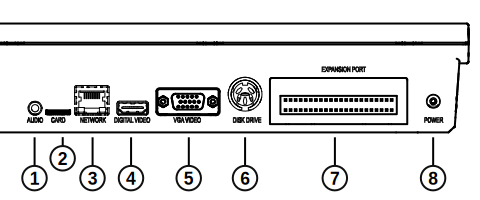
\includegraphics[width=\linewidth]{images/illustrations/mega65-rear.pdf}
\begin{center}
\setlength{\def\arraystretch{1.5}\tabcolsep}{6pt}
\begin{longtable}{ c | l}
	1	& 	3.5mm Audio Jack \\
	2	& 	External microSD Card Slot\\
	3	& 	Network LAN Port \\
	4	& 	Digital Video Connector (including sound) \\
	5	& 	VGA Video Connector \\
	6	& 	IEC Serial Bus Connector for Disk Drives and Printers \\
	7	& 	Cartridge Expansion Port \\
	8	& 	Power Supply Socket \\
\end{longtable}
\end{center}

\vspace{-1cm}

\section{Side Connections}

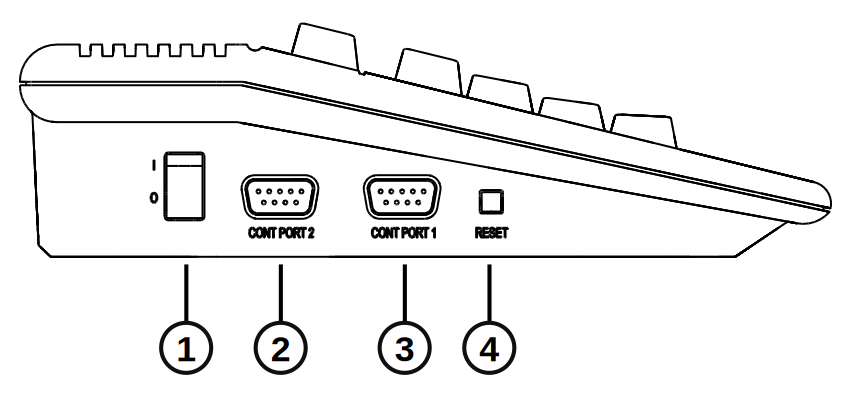
\includegraphics[width=\linewidth]{images/illustrations/mega65-side.pdf}

\begin{center}
\setlength{\def\arraystretch{1.5}\tabcolsep}{6pt}
\begin{longtable}{ c | l}
	1	& 	Power Switch \\
	2	& 	Controller Port 2 \\
	3	& 	Controller Port 1 \\
	4	& 	Reset Button \\
\end{longtable}
\end{center}

Various peripherals can be connected to Controller Ports 1 and 2 such as
joysticks, paddles or mouse devices.

\newpage

\section{MEGA65 Screen and Peripherals}

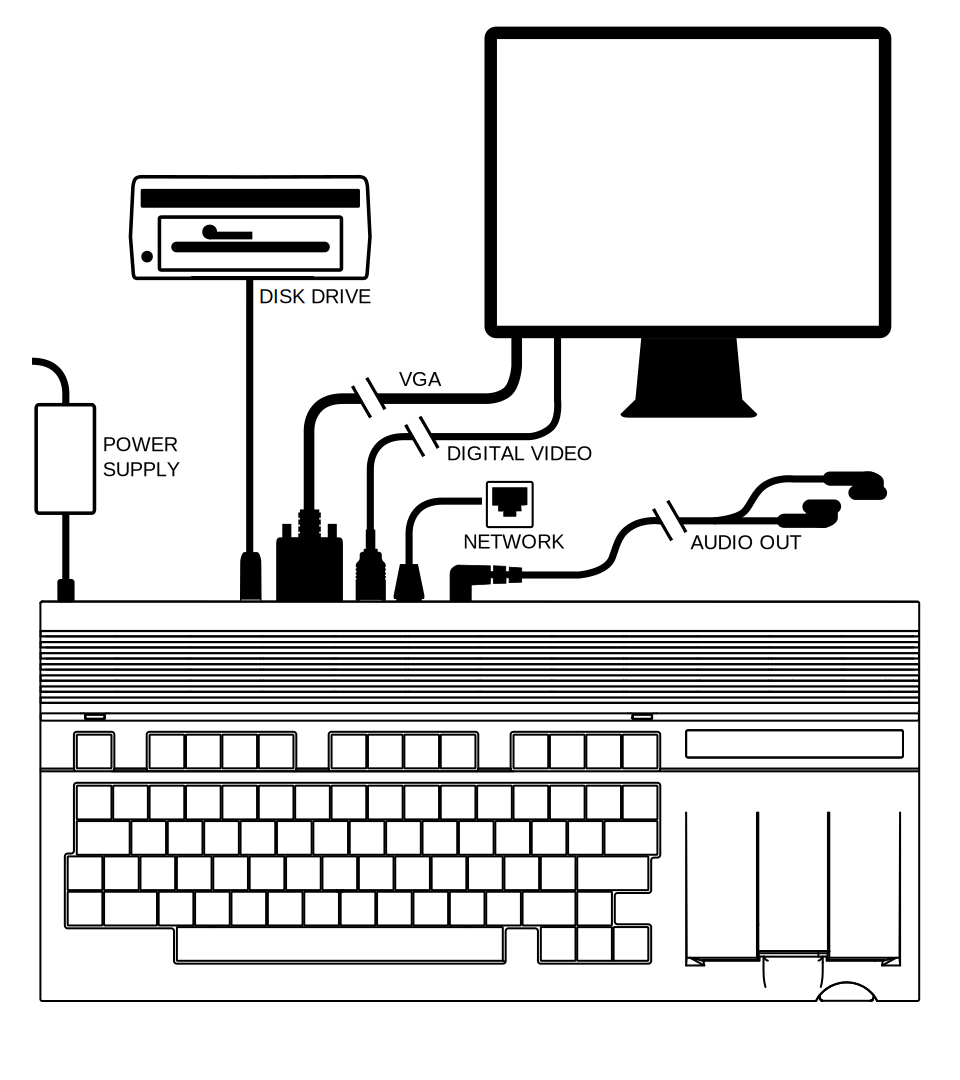
\includegraphics[width=\linewidth]{images/illustrations/mega65-top.pdf}

To connect your MEGA65 to a display:
\index{Display!Connecting}

\begin{enumerate}
	\item Connect the power supply to the power supply socket of the MEGA65.
	\item If you have a VGA monitor and a VGA cable, connect one end to the VGA port of the MEGA65 and the other end into your VGA monitor.
	\item If you have a TV or monitor with a compatible Digital Video connector,\footnote{The Digital Video connector type has a recognizable four-letter commercial name, but the MEGA65 project has not paid the licensing fees to refer to it by this name. This {\em User's Guide} refers to this as the ``Digital Video'' connector.}\index{Digital Video} connect one end of your cable to the Digital Video port of the MEGA65, and the other into the Digital Video port of your monitor. If you own a monitor with a DVI socket, you can use a Digital Video to DVI adapter.
\end{enumerate}

\newpage
\section{Optional Connections}
\index{Disk Drives!Connecting}
\index{Connections!IEC}
\index{SD Cards!Locations}
\begin{enumerate}
	\item The MEGA65 includes an internal 3.5" floppy disk drive. You can also connect older Commodore{\textregistered} IEC serial floppy drives to the MEGA65, such as the Commodore 1541, 1571 or 1581. To use these drives, connect one end of an IEC cable to the Commodore floppy disk drive and the other end to the Disk Drive socket of the MEGA65. You can also connect an SD2IEC device\index{SD2IEC device} or a Pi1541 device.\index{Pi1541 device} With most devices, you can daisy-chain additional floppy disk drives or Commodore compatible printers.
	\item You can connect your MEGA65 to an Ethernet network using a standard Ethernet cable.
	\item For enjoying audio from your MEGA65, you can connect a 3.5mm audio jack cable to an audio amplifier or speaker system. If your system has RCA connectors you will need a 3.5mm audio jack to twin RCA adapter cable. The MEGA65 also has a built-in amplifier to allow the use of headphones.
	\item A microSD card, type SDHC between 4GB and 32GB, can be inserted into the external microSD card slot at the rear of the MEGA65. For more information on using the microSD card slot, see ``Introducing SD Cards'' on page \pageref{sec:introducing-sd-cards}.
	\item Underneath the MEGA65, a small door provides access to the internal SD card and two connectors for future hardware expansion.
\end{enumerate}

\index{Real-Time Clock!Installing the Battery}
\subsection{Installing the Real-Time Clock Battery}

The MEGA65 includes a Real-Time Clock, which is used to display the time and date on the startup screen, to add timestamps to files that the MEGA65 writes to your SD cards, and by the {\bf DT\$}\index{BASIC 65 Variables!DT} and {\bf TI\$}\index{BASIC 65 Variables!TI\$} BASIC65 variables. This clock utilises a CR2032 coin-cell battery\footnote{Early models of MEGA65 with the "R3A" board revision used a battery of type CR1220 for the Real-Time Clock. Revisions "R5" and later, which began shipping in late 2023, use a CR2032 battery.} to keep time when the MEGA65 isn't switched on. The MEGA65 does not include a battery in order to avoid issues related to shipping batteries internationally.

To install the battery, use a Phillips-head screwdriver to open the case, exposing the motherboard.\index{Case!Opening} The case is held together with three screws, all of which are along the bottom of the front side of the case. Once the screws have been removed, carefully lift the top half of the case. Note the orientation of the keyboard connector, then disconnect it.

The battery is located between the controller ports and the keyboard connector.

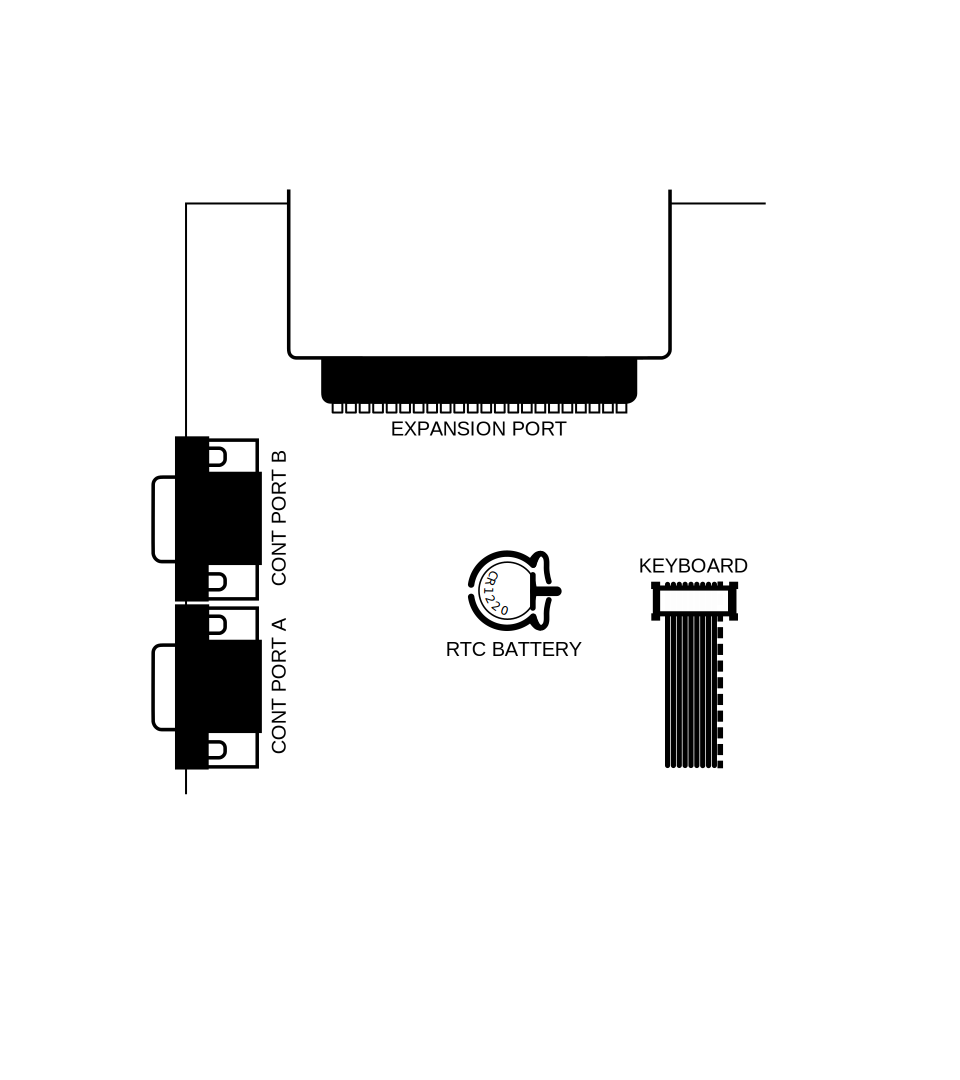
\includegraphics[width=\linewidth]{images/illustrations/rtc-battery-location.pdf}

If you are removing an existing battery, push the battery release lever on the bottom (flat-sided) side of the battery socket away from the battery to remove it. Insert the new battery with the side labelled {\bf +} facing up, and press it into place.

Once you have re-assembled your MEGA65, you can set the time in the Configuration Utility. For more information on how to set the Real-Time Clock, refer to the Configuration Utility section on page \pageref{sec:configuration-utility}.


\newpage

\section{Switching the MEGA65 on for the First Time}
\label{onboarding}

Switch the MEGA65 on using the power switch on the left-hand side of the computer.

When you switch your MEGA65 on for the first time, it displays the initial configuration (``on-boarding'') screen.\index{Configuration!On-boarding} You can use this screen to set the time and date on the Real-Time Clock (if you have installed the CR2032 battery), change the video display mode, and test the audio. All of these settings can be changed later.

\begin{center}
  \includegraphics[width=0.7\linewidth]{images/img011_final_boot_01.png}
\end{center}

For video display modes, you can select between PAL\index{PAL display mode} or NTSC\index{NTSC display mode} emulation, and you can select whether your Digital Video display supports sound. If you are using the VGA video output, the Digital Video sound mode has no effect.

\underline{Note}: A DVI display that does not support sound will not work with the ``enhanced'' sound mode. With such a display, you must select a video mode with ``no sound,'' and connect a speaker to the 3.5 mm audio jack.

PAL and NTSC are analog video signal formats that affect the resolution and vertical sync speed of the video output, even when using a modern digital display. Your display may support either mode, or it may only support one or the other. You can use this screen to test the modes with your display.

Select and test your video configuration. For example, press \specialkey{TAB} to switch to the {\bf PAL 50HZ} mode.
\index{Display!Setting PAL/NTSC}
\begin{center}
  \includegraphics[width=0.7\linewidth]{images/img011_final_boot_02.png}
\end{center}

Press \megakey{SPACE} followed by \megakey{Y} to test the new video mode.

\begin{center}
  \includegraphics[width=0.7\linewidth]{images/img011_final_boot_03.png}
\end{center}

Press \megakey{K} to keep the new video mode.

\begin{center}
  \includegraphics[width=0.7\linewidth]{images/img011_final_boot_04.png}
\end{center}

Take this opportunity to test your sound set-up. Press \megakey{A} to play a sound.

The ``CRT emulation'' option is a fun choice when using a modern flat panel display. It adds vertical gaps between pixels to simulate the CRT raster line. Try it to see if you like it: press the \megakey{C} key to toggle it on and off.

Finally, press \specialkey{RETURN} to complete the configuration.

For more information about configuring your MEGA65, see chapter \vref{cha:configuringyourmega}.

\section{The Intro Disk}
\index{Intro Disk}

After completing the on-boarding configuration, your MEGA65 starts the Intro Disk menu. The Intro Disk is a collection of software made by the MEGA65 community that demonstrates some of the capabilities of the computer. Take some time to browse the menus and try some of the demos. After each demo, press the reset button on the left-hand side of the computer to return to the Intro Disk menu.

\begin{center}
  \includegraphics[width=0.7\linewidth]{images/demo_title.png}
\end{center}

By default, the Intro Disk menu opens each time you switch on the computer. Once you are more familiar with the MEGA65, you may wish to disable this. Press \megakey{D} at the Intro Disk menu to disable its auto-boot feature.\index{Intro Disk!Disabling}

Press \megakey{X} to exit the Intro Disk menu and access BASIC 65. With the Intro Disk auto-boot feature disabled, the MEGA65 goes directly to BASIC 65 when you switch it on.

\begin{center}
  \includegraphics[width=0.7\linewidth]{images/img011_final_boot_06.png}
\end{center}

\section{The Cursor}

The flashing square underneath the \screentext{READY} prompt\index{READY prompt} is called the cursor. The cursor indicates that the computer is ready to accept input. Pressing keys on the keyboard will print their respective characters onto the screen. The characters will be printed at the current cursor position, and the cursor will advance to the next position after every key press.

Here you can type commands, that can do things such as loading a program. You can also start entering program code!

\chapter{Getting Started}
\addtocontents{toc}{\protect\setcounter{tocdepth}{2}}
\hypersetup{bookmarksdepth=5}

\section{Keyboard}
\label{cha:getting-started}
\index{Keyboard}

Now that everything is connected, it's time to get familiar with the MEGA65 keyboard.

You may notice that the keyboard is a little different to the keyboards used on computers today. While most keys will be in familiar positions, there are some specialised keys, and some with special graphic symbols marked on the front.

The graphic symbols are typable in some display modes, similar to letters, numbers, and punctuation. The complete set of characters is known as the {\em PETSCII character set}.\index{PETSCII}

\subsection{Special Keys}

\subsubsection{RETURN}
\index{Keyboard!RETURN}
Pressing \specialkey{RETURN} enters the information you have typed into the MEGA65's memory. The computer will either act on a command, store some information, or display an error message if you made a mistake.

\subsubsection{SHIFT}
\index{Keyboard!Shift Keys}
The two \specialkey{SHIFT} keys are located on the left and the right. They work very much like the Shift key on a regular keyboard. They also perform some special functions as well.

In upper case mode, holding down \specialkey{SHIFT} and pressing any key with two graphic symbols on the front produces the right-hand symbol on that key. For example, \specialkey{SHIFT} and \megakey{J} prints the \graphicsymbol{J} character.

In lower case mode, pressing \specialkey{SHIFT} and a letter key prints the upper case letter on that key.

Finally, holding \specialkey{SHIFT} down and pressing a Function key accesses the function shown on the front of that key. For example: \specialkey{SHIFT} and \megakey{F1} activates \megakey{F2}.


\subsubsection{SHIFT LOCK}
\index{Keyboard!SHIFT LOCK}
In addition to \specialkey{SHIFT} is \specialkey{SHIFT\\LOCK}. Press this key to lock down the Shift function. Now any key you press while \specialkey{SHIFT\\LOCK} is illuminated prints the character to the screen as if you were holding down \specialkey{SHIFT}. This includes special graphic characters.

\subsubsection{CTRL}
\index{Keyboard!CTRL}
\specialkey{CTRL} is the Control key. Holding down \specialkey{CTRL} and pressing another key allows you to perform Control functions. For example, holding down \specialkey{CTRL} and one of the number keys (from \megakey{1} to \megakey{8}) allows you to change text colours. The colour that is printed at the top row on the front of the number key will be used. Holding down \specialkey{CTRL} and pressing \megakey{9} or \megakey{0} switches reverse-text mode on and off.

There are some examples of this on page \pageref{sec:screen-editor}, and all of the Control functions are listed on page \pageref{appendix:controlcodes}.

If a program is being {\bf LIST}ed to the screen, holding down \specialkey{CTRL} slows down the display of each line. You can read more about the {\bf LIST} command on page \pageref{BASIC 65 Commands!LIST}.\index{BASIC 65 Commands!LIST}

Holding \specialkey{CTRL} and pressing \megakey{*} enters the Matrix Mode Debugger (refer to the {\bf MEGA65 Book} for more details).

\subsubsection{RUN STOP}
\index{Keyboard!RUN STOP}
Normally, pressing \specialkey{RUN STOP} stops the execution of a program. Holding \specialkey{SHIFT} while pressing \specialkey{RUN STOP} {\bf RUN}s the first program from disk.\index{BASIC 65 Commands!RUN}

Some programs override the \specialkey{RUN STOP} key and cannot be stopped in this way.

You can boot your MEGA65 into the {\bf Machine Code Monitor}\index{Machine Code Monitor} by holding down \specialkey{RUN STOP} and pressing reset on the left-hand side.

\subsubsection{RESTORE}
\index{Keyboard!RESTORE}
The computer screen can be restored to a clean state without clearing the memory by holding down \specialkey{RUN STOP} and pressing \widekey{RESTORE}. This combination also resets operating system vectors and re-initialises the screen editor, which makes it a handy combination if the computer has become a little confused.

Some programs override the \specialkey{RUN STOP} + \widekey{RESTORE} key combination and cannot be reset in this way.

You can also enter the {\bf Freezer} by pressing and holding \widekey{RESTORE} for half to one second. You can
read more about the Freezer on page \pageref{sec:freezer}.\index{Freezer menu}

\subsubsection{THE CURSOR KEYS}
\index{Keyboard!Cursor Keys}
\nopagebreak
At the bottom right-hand side of the keyboard are the cursor keys. These four directional keys allow you move the cursor to any position for on-screen editing.

The cursor moves in the direction indicated on the keys: \megakey{$\leftarrow$} \megakey{$\uparrow$} \megakey{$\rightarrow$} \megakey{$\downarrow$}.

You don't have to keep pressing a cursor key over and over. If you need to move the cursor a long way, you can keep the key pressed down. When you are finished, simply release the key.

\subsubsection{ARROW KEYS}
\index{Keyboard!Arrow Keys}
These keys are different to the cursor keys! They are \megakeywhite{$\leftarrow$} (next to \megakey{1}), and \megakeywhite{$\uparrow$} (next to \widekey{RESTORE}).
Both arrow keys are used in various BASIC functions and escape sequences.

For example, \megakeywhite{$\leftarrow$} can be used as a shortcut for {\bf SAVE},\index{BASIC 65 Commands!SAVE} and \megakeywhite{$\uparrow$} is used to raise a number to a power (which is the same as multiplying a number by itself a specified number of times).

You can read more about the available escape sequences on page \pageref{escape-sequences}.

These two PETSCII specific keys will always be shown in MEGA65 literature with a white background.

It is also possible to move the cursor up by using \specialkey{SHIFT} and \megakey{$\downarrow$}, and left by using \specialkey{SHIFT} and \megakey{$\rightarrow$}. This owes to the MEGA65's Commodore 64 heritage, which only had two cursor keys.

\subsubsection{INSerT/DELete}
\index{Keyboard!INST DEL}
This is the INSERT / DELETE key. When pressing \specialkey{INST\\DEL}, the character to the left is deleted, and all characters to the right are shifted one position to the left.

To insert a character, hold \specialkey{SHIFT} and press \specialkey{INST\\DEL}. All the characters to the right of the cursor are shifted to the right. This allows you to type a letter, number or any other character at the newly inserted space.


\subsubsection{CLeaR/HOME}
\index{Keyboard!CLR HOME}
Pressing \specialkey{CLR\\HOME} places the cursor at the top left-most position of the screen.

Holding down \specialkey{SHIFT} and pressing \specialkey{CLR\\HOME} clears the entire screen {\it and} places the cursor at the top left-most position of the screen.

If you press \specialkey{CLR\\HOME} accidentally, you can return the cursor to its prior position by pressing \specialkey{ESC} then \specialkey{CLR\\HOME}.

\subsubsection{MEGA KEY}
\index{Keyboard!MEGA Key}
\megasymbolkey or the MEGA key provides a number of different functions and can be used to launch special utilities.

Holding \specialkey{SHIFT} and pressing \megasymbolkey switches between lower and uppercase character modes.

Holding \megasymbolkey and pressing any key with two graphic symbols on the front prints the left-most graphic symbol to the screen. For example,
\megasymbolkey and \megakey{D} prints the \graphicsymbol{d} symbol.

Holding \megasymbolkey and pressing any key that shows a single graphic symbol on the front prints that graphic symbol to the screen.

Holding \megasymbolkey and pressing a number key switches to one of the colours in the second range, i.e., the colour that is printed at the bottom row on the front of the number key will be used.

Holding \megasymbolkey and pressing \specialkey{TAB} enters the Matrix Mode Debugger (refer to the {\bf MEGA65 Book} for more details).

Switching on the MEGA65 or pressing the reset button on the left-hand side while holding down \megasymbolkey switches the MEGA65 into GO64 mode.\index{Commodore 64!GO64 mode}

\subsubsection{NO SCROLL}
\index{Keyboard!NO SCROLL}
If a program is being {\bf LIST}ed to the screen, pressing \specialkey{NO\\SCROLL} pauses the screen output. Press any key to un-pause.

This feature is not available in GO64 mode.\index{Commodore 64!GO64 mode}

\subsubsection{FUNCTION KEYS}
\index{Keyboard!Function Keys}
There are seven Function keys available for use by software applications. \megakey{F1} \megakey{F3} \megakey{F5} \megakey{F7} \megakey{F9} \megakey{F11} and \megakey{F13} can be used to perform special functions.

Hold \specialkey{SHIFT} to access \megakey{F2} through to \megakey{F14} as shown on the front of each Function key.
\index{Keyboard!Shift Keys}
Only Function keys \megakey{F1} to \megakey{F8} are available in GO64 mode.\index{Commodore 64!GO64 mode}

\subsubsection{HELP}
\index{Keyboard!HELP}
\specialkey{HELP} can be used by software and also acts as \megakey{F15} / \megakey{F16}.

\subsubsection{ALT}
\index{Keyboard!ALT}
Holding \specialkey{ALT} down while pressing other keys can be used by software to perform specific functions. This feature is not available in GO64 mode.\index{Commodore 64!GO64 mode}

Holding \specialkey{ALT} down while switching the MEGA65 on activates the Utility Menu.\index{Utility menu} You can format an SD card, or enter the MEGA65 Configuration Utility\index{Configuration!Utility} to select the default video mode and change other settings, or to test your keyboard.

\subsubsection{CAPS LOCK}
\index{Keyboard!CAPS LOCK}
\specialkey{CAPS\\LOCK} works similarly to \specialkey{SHIFT\\LOCK} in C65 and MEGA65-modes, but only modifies the letter keys.

When the MEGA65 is set to run at a reduced processor speed, such as in GO64 mode,\index{Commodore 64!GO64 mode} you can hold down \specialkey{CAPS\\LOCK} to run the processor at full speed temporarily. This is useful in GO64 mode for things such as
speeding up loading from the internal disk drive or SD card, or to greatly speed up the de-packing process after a program is run. MEGA65 mode runs at maximum speed by default.

\addtocontents{toc}{\protect\setcounter{tocdepth}{5}}


\section{The Screen Editor}
\label{sec:screen-editor}

When you switch on your MEGA65 or reset it, the following screen will appear:\footnote{This assumes you have disabled the Intro Disk menu. If the Intro Disk menu is running, press ``X'' to exit to this screen.}

\begin{center}
\includegraphics[width=0.9\linewidth]{images/introduction-screen/layout.png}
\end{center}

The colour bars in the top left-hand side of the screen can be used as a guide to help calibrate the colours of your display. The screen also displays the name of the system, the copyright notice, and the ROM version. The displayed date and time are taken from the internal RTC (Real-Time Clock) at the time the computer was powered on. You can set the date and time in the Configure Utility.

Finally, you will see the \screentext{READY} prompt and the flashing cursor.

You can begin typing keys on the keyboard and the characters will be printed at the cursor position. The cursor itself will advance after each key press.

You can also produce reverse text or colour bars by holding down \specialkey{CTRL} and pressing \megakey{9}, or \megakey{R}. This enters reverse text mode. When this is enabled, you can press and hold the \megakey{Space} bar. While doing so, a white bar will be drawn across the screen.
\index{Keyboard!CTRL}
You can change the current colour by holding \specialkey{CTRL} down and pressing a number key (from \megakey{1}
to \megakey{8}). For example, if you press and hold \specialkey{CTRL} down and press \megakey{1}, the colour will
change to black. Now, when you hold down the \megakey{Space} bar, a black bar will be drawn. If you continue to
change the colour and press the \megakey{Space} bar, you will get an effect similar to the following image:

\begin{center}
\includegraphics[width=0.7\linewidth]{images/introduction-screen/colour-bars.png}
\end{center}

You can disable reverse text mode by holding \specialkey{CTRL} and pressing \megakey{0}.

A further eight colours can be selected by holding down \megasymbolkey and pressing a key from \megakey{1} to \megakey{8}.\index{Keyboard!MEGA Key}

The colour that is printed at the bottom row on the front of the number key will be used. For example, if you held
\megasymbolkey down while pressing \megakey{4}, dark grey will be used. For access to an additional 16 colours of the alternate/rainbow palette, refer to the \specialkey{CTRL} + \megakey{A} shortcut described on page \pageref{appendix:controlcodes}.

\underline{NOTE}:
\begin{itemize}
  \item {\bf Quote Mode}: If you were to press \megakey{"} to open a string, and then try to change
colours, reverse text, move the cursor keys, or use the \specialkey{CLR HOME} key, instead
of these actions instantly occurring, funny PETSCII\index{PETSCII} symbols will appear instead. This is
due to a BASIC facility called {\it quote mode} (described further in the \textbf{MEGA65 Book}),
which allows you to encode such actions into a string so that they can be executed at a later
time (for example, via a {\bf PRINT} statement within your programs). To end {\it quote mode}, simply
type another \megakey{"} to mark the end of your string.
  \item {\bf Insert Mode}: A similar facility is called
{\it insert mode}, where for the number of times you press \specialkey{SHIFT} + \specialkey{INST\\DEL}
to insert a few spaces, the same number of keypresses that follow it will abide by the same
principles of {\it quote mode}.
  \item You can forcefully exit either of these modes by pressing \specialkey{ESC}, \megakey{O}.
\end{itemize}

\needspace{4cm}
You can create fun pictures just by using these colours and letters. Here's an example of what a 4th year student drew:

\begin{center}
\includegraphics[width=0.7\linewidth]{images/caleb-PETSCII-TNT-final}
\end{center}

What will you draw?

\needspace{2cm}
\textbf{Functions}

Functions using \specialkey{CTRL} are called \textbf{Control Codes}.
Functions using \megasymbolkey are called \textbf{Mega Codes}. There are also functions that are called by using \specialkey{SHIFT}, which are called \textbf{Shifted Codes}.

Lastly, \specialkey{ESC} enables the use of \textbf{Escape Sequences}.

You can read about all of these functions in detail on page \pageref{appendix:controlcodes}.

\needspace{2cm}
\textbf{ESC Sequences}

\index{Keyboard!Escape Sequences}
Escape sequences are performed a little differently than a Control function or a Shift function. Instead of holding the modifier key down, an Escape sequence is performed by pressing \specialkey{ESC} and releasing it, followed by pressing the desired key.

For example: to switch between 80 column mode and 40 column mode, press and release \specialkey{ESC}, then press \megakey{X}.

There are more text modes available. You can create flashing text by holding \specialkey{CTRL} down and pressing \megakey{O}. Any characters you type in will flash. Turn flash mode off by pressing \specialkey{ESC}, then \megakey{O}.


\section{Editor Functionality}

The MEGA65 screen editor\index{Screen editor} supports several ways to quickly move the cursor around the screen to help you to be more productive.

For example, press \specialkey{CLR HOME} to go to the home position on the screen. Hold \specialkey{CTRL} down and press \megakey{W} several times. This is the \textbf{Word Advance function}, which jumps your cursor to the next word, or printable character.

You can set custom tab positions on the screen for your convenience. Press \specialkey{CLR HOME} and then \megakey{$\rightarrow$} to move the cursor to the fourth column. Hold down \specialkey{CTRL} and press \megakey{X} to set a tab. Move another 16 positions to the right, and press \specialkey{CTRL} and \megakey{X} again to set a second tab.

Press \specialkey{CLR HOME} to go back to the home position. Hold \specialkey{CTRL} down and press \megakey{I}. This is the \textbf{Forward Tab function}. Your cursor will tab to the fourth position. Press \specialkey{CTRL} and \megakey{I} again. Your cursor will move to position 8. By default, every 8th position is already set as a tabbed position. So the 4th and 20th positions have been added to the existing tab positions. You can continue to press \specialkey{CTRL} and \megakey{I} to advance to the 16th and 20th positions.

\subsection{Creating a Window}
\index{Keyboard!Escape Sequences}
\index{Windows!Escape sequences}

You can set a window on the MEGA65 working screen. Move your cursor to the beginning of the "BASIC 65" text. Press \specialkey{ESC}, then press \megakey{T}. Move the cursor 10 lines down and 15 to the right.

Press \specialkey{ESC}, then \megakey{B}. Anything you type will be contained within this window.

For example, if you were to type \screentext{LIST} to list out a program, the listing will be confined to the window region you have specified:

\begin{center}
\includegraphics[width=0.7\linewidth]{images/set-window.png}
\end{center}

To escape from the window back to the full screen, press \specialkey{CLR HOME} twice.

\subsection{Additional ASCII characters}

You may have noticed a few ASCII characters on the MEGA65 keyboard that aren't traditionally a part of the PETSCII character set.\index{PETSCII} In order to make use of these from within BASIC:

\begin{itemize}
  \item Type either \screentext{FONT A} or \screentext{FONT B}.
  \item Press \megasymbolkey + \specialkey{SHIFT} to switch to lowercase.
\end{itemize}

You will now be able to type those additional ASCII characters via the keyboard. To revert back to the original PETSCII character set, type \screentext{FONT C}.

\subsection{Uppercase and lowercase}

\megasymbolkey + \specialkey{SHIFT} switches between uppercase and lowercase text for the entire display. This works even during program execution, so you can adjust it if a program is in the wrong mode.


\section{The Freezer Menu}
\label{sec:freezer}
\index{Freezer menu}
\nopagebreak
The MEGA65 spends most of its time behaving as a Commodore 65 computer would, either running a program or awaiting instructions in the BASIC environment. Your MEGA65 has additional features that were not part of the original C65 design. You can access many of these features from the Freezer menu.

To open the Freezer menu, hold the \widekey{RESTORE} key for one second, then release it. The MEGA65 will pause whatever it is doing, flicker the border colour, then open the Freezer menu. Whatever program was running remains in memory and can be resumed by pressing the \specialkey{F3} key. You can also abandon the running program and reset the MEGA65 by pressing \specialkey{F5}.

\begin{center}
  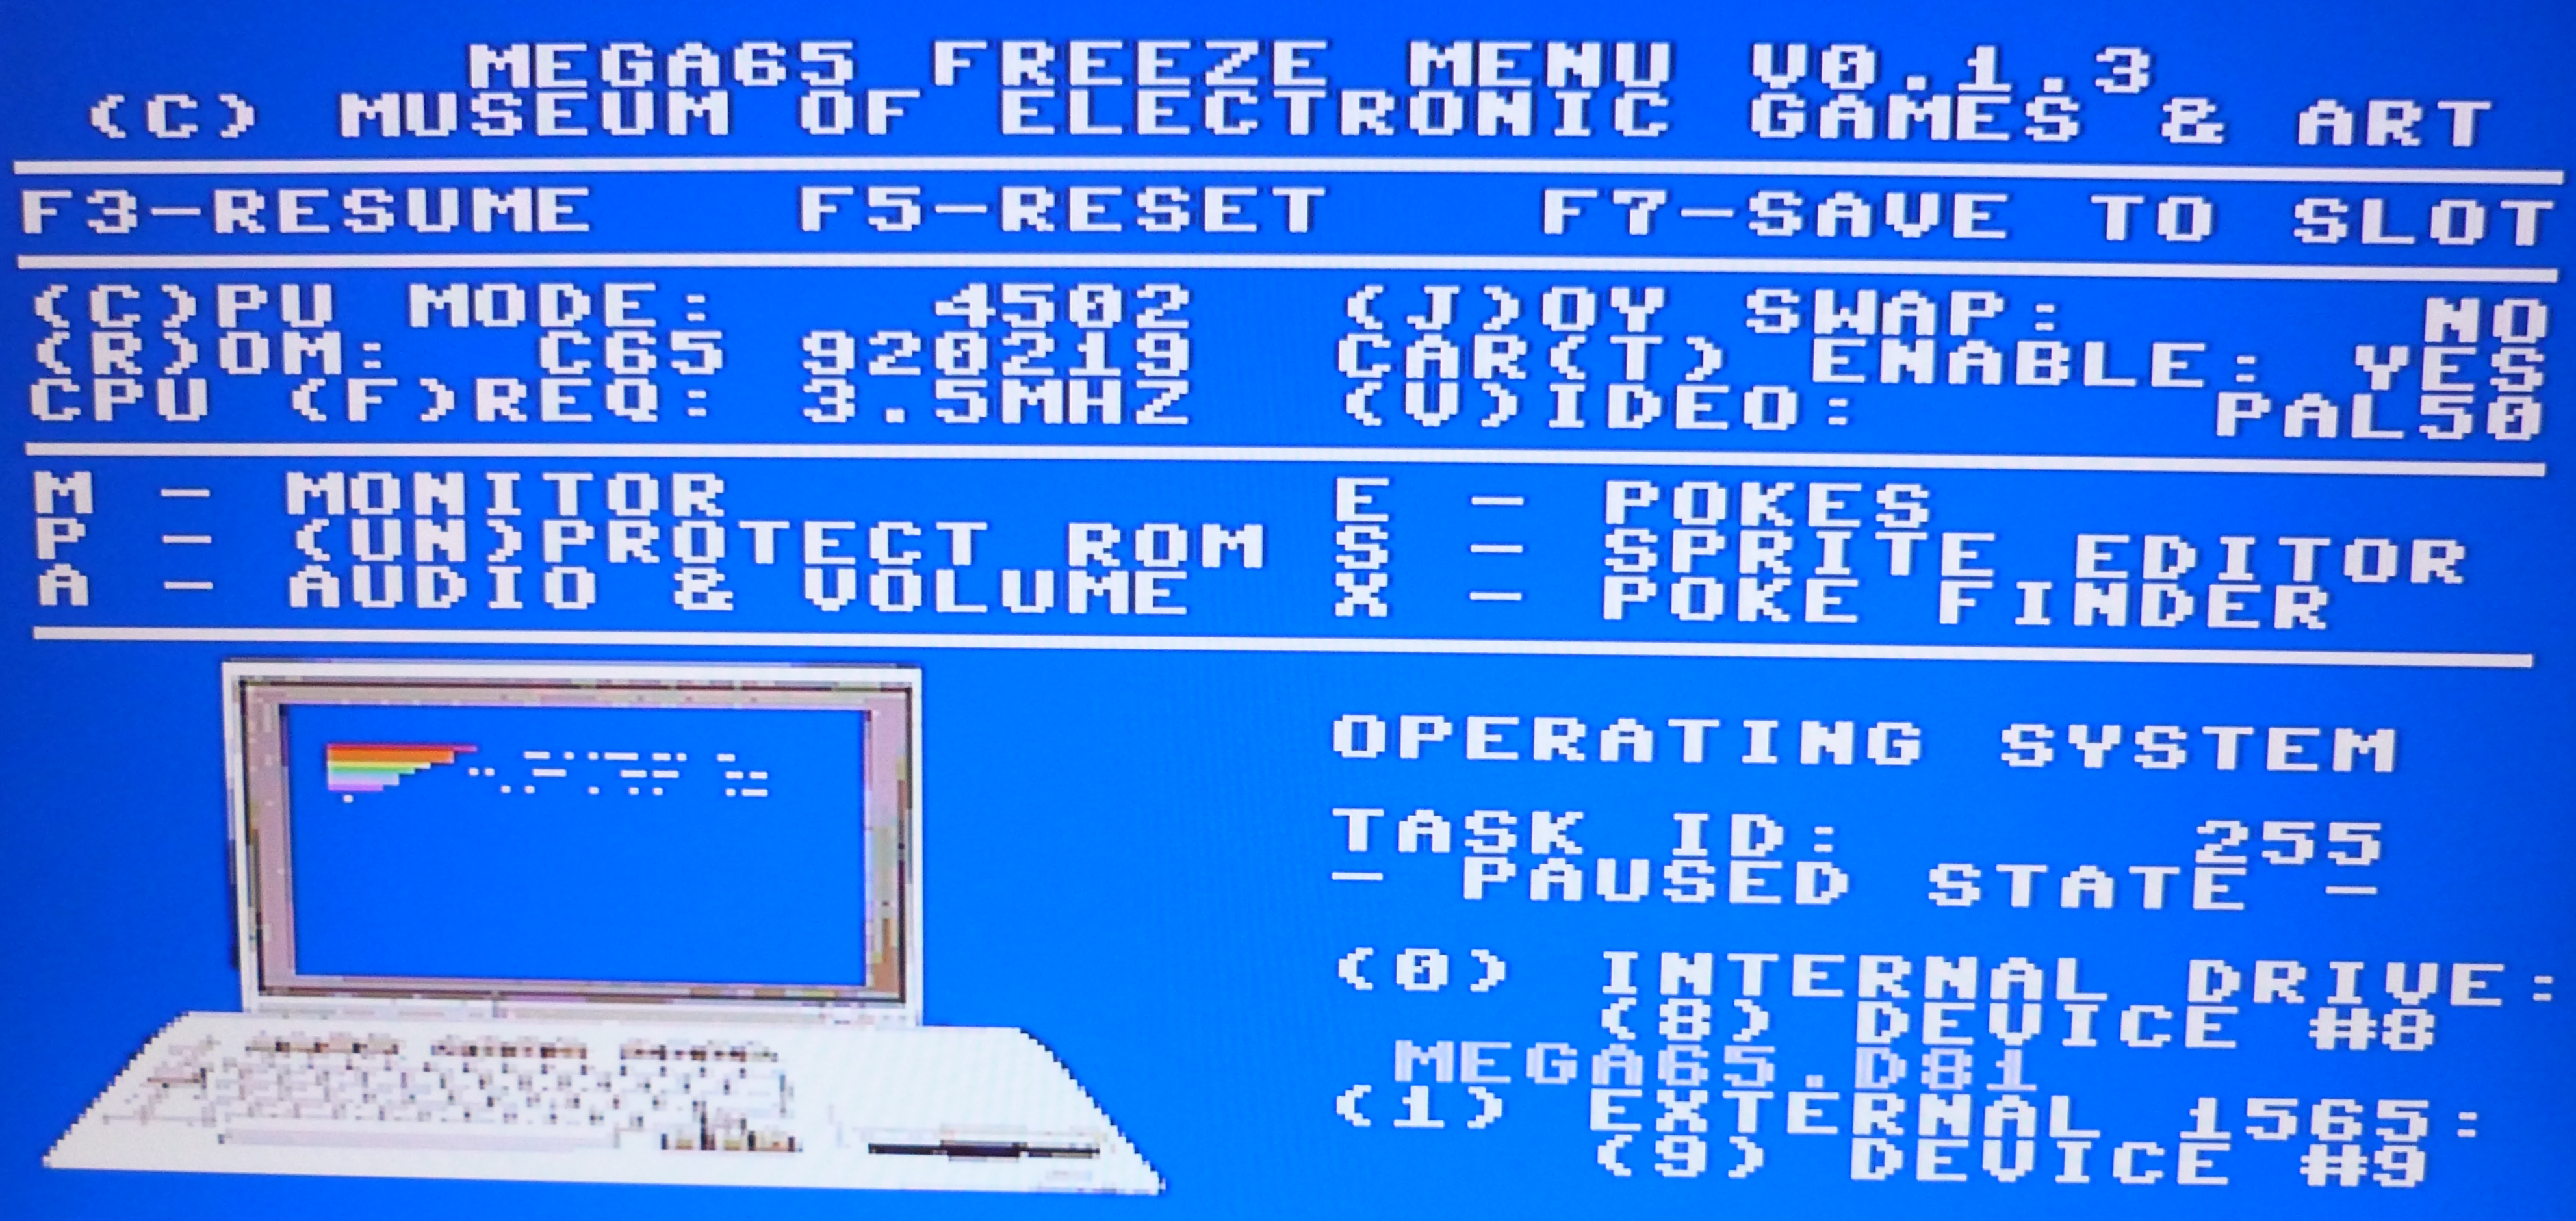
\includegraphics[width=0.7\linewidth]{images/freezer.png}
\end{center}

One feature to remember when playing games is the ``(J)OY SWAP.'' This causes the two joystick ports to trade numbers. If you have a joystick in port 2 and you start a game that expects a joystick in port 1, instead of disconnecting and reconnecting the joystick, open the Freezer menu, press \megakey{J} to swap the port numbers, then resume your game.

This is called the ``Freezer'' menu because the state of the MEGA65 remains frozen while using it. The Freezer menu can store multiple freeze states, and you can switch between them. To save the current state, navigate to an unused {\it freeze slot} using the cursor-right key, then press \megakey{F7}. When the border stops blinking, the state is saved. To restore a state, navigate to the freeze slot, then press \megakey{F3} to resume operation.

The Freezer menu has several built-in options and features. For more information about the MEGA65 Information Utility (``MEGAINFO''), see ``Determining the Versions of Things'' on page \pageref{sec:versions}. For more information about mounting disks and disk images, see chapter \vref{cha:using-disks}.


\section{Running Commodore 64 Software}

The MEGA65 is capable of running Commodore 64 software. There are two ways to do this: the built-in GO64 mode, and the {\it C64 for MEGA65} FPGA core.

\subsection{GO64 Mode}
\index{Commodore 64!GO64 mode}

The original Commodore 65 was designed to be capable of running some Commodore 64 software. The MEGA65 supports this feature, known as ``GO64 mode.''

\underline{NOTE}: Due to how Commodore designed this feature, not all C64 software is compatible with this mode. Unlike the similar feature of the Commodore 128, the Commodore 65 uses a different CPU, and minor differences are known to cause compatibility issues with some software titles.

There are three ways to switch the MEGA65 into GO64 mode:

\begin{itemize}
    \item Switch off the computer, hold the \megasymbolkey and switch it back on.
    \item From the MEGA65 \screentext{READY} prompt, enter this command: \screentext{GO64} Enter \screentext{YES} when prompted.\index{BASIC 65 Commands!GO64}
    \item Switch off the computer, connect a Commodore 64 cartridge to the expansion port, then switch the computer on.
\end{itemize}

\begin{center}
  \includegraphics[width=0.7\linewidth]{images/go64.png}
\end{center}

GO64 mode is actually just a temporary re-configuration of the MEGA65. All of the MEGA65's features are still present, including the Freezer menu for mounting D81 disk images.

Much Commodore 64 software can be found on the Internet in the form of D64 disk images. The MEGA65 only supports D81 disk images via the SD card and Freezer menu. You can use a peripheral such as the SD2IEC\index{SD2IEC device} with the MEGA65's IEC port to use D64 disk images. Be sure to obtain an SD2IEC with an independent power supply, and not one that depends on a Commodore 64 tape connector.\footnote{For more information on SD2IEC devices, see: \url{https://www.c64-wiki.com/wiki/SD2IEC}}

\subsection{The ``C64 for MEGA65'' FPGA Core}
\index{Core!C64 core}\index{Commodore 64!Core}

The {\it C64 for MEGA65} FPGA core by MJoergen and sy2002 re-creates the original Commodore 64 computer on MEGA65 hardware with a high degree of accuracy. It does so by completely replacing the MEGA65 core with one that implements the Commodore 64 chipset, including its CPU. MEGA65 features such as the Freezer menu are not available when running the C64 core. Instead, the core provides its own menu for mounting D64 disk images and other features. Press the \specialkey{HELP} key with the core running to access this menu.

% TODO: When the cartridge-to-core configuration feature is complete:
% With the C64 core installed, you can configure the MEGA65 boot process to use the core when a Commodore 64 cartridge is connected, instead of using the less-compatible GO64 mode. ...
% (Refer to chapter \vref{cha:cores})

For information about installing FPGA cores, see chapter \vref{cha:cores}. To download the {\it C64 for MEGA65} core and read important installation instructions, see: \url{https://github.com/MJoergen/C64MEGA65}

\chapter{Configuring your MEGA65}
\label{cha:configuring}

\section{Important Note}

For your convenience, your MEGA65 comes with an SD card with all of the essential
files already on it, so you may prefer to skip this section and jump straight to
the on-boarding section on page \pageref{onboarding}.

Alternatively, you're welcome to read this section and familiarise
yourself on how your SD card was prepared.

{\bf Do not format the SD card that came with your MEGA65}.
If you want to create a new bootable SD card, please use another one,
and keep the SD card that came with your MEGA65 as a safety backup.

\section{Formatting SD cards}
\index{SD Cards!Formatting}
The MEGA65 has two SD card slots: A full-size SD card slot inside, under
the trap-door, and a microSD size slot on the rear.  The current version
of the MEGA65 firmware only supports the use of one SD card at a time.
If you have cards in both slots, the MEGA65 will default to the external slot. The exception to this is that the MEGA65's FDISK/FORMAT
utility can access both, allowing you to select which SD card to format or
repair.

If you wish to use a different SD card to the pre-configured one supplied with your MEGA65, the new SD card must be formatted first.

{\bf This must be done on the MEGA65, not on a PC or other computer.}

{\em Only use SDHC cards. Older SD cards (typically with
  a capacity of <4GB) will not work. Newer SDXC cards with
  capacities greater than 32GB may or may not work. We would
  appreciate hearing your experience with such cards. It is unimportant
  as to which file-system is currently on the card, as the MEGA65
  FDISK/FORMAT utility will completely reformat the card.}

There are several reasons for this: First, to fit the most
features into the MEGA65's small operating system, it is
particular about the FAT32 file system it uses. Second, only the
MEGA65 FDISK/FORMAT utility can create a MEGA65 System Partition. The
MEGA65 System Partition holds non-volatile configuration settings for
your MEGA65, and also contains the freeze slots that make it easy to
switch between MEGA65 programs and games.

Formatting an SD card on the MEGA65 is easy. Switch the MEGA65 on while holding \specialkey{ALT} down.

This will present the MEGA65 Utility Menu, which contains a
selection of built-in utilities, similar to the following:

%\begin{wrapfigure}{l}{0.7\textwidth}
\begin{center}
\includegraphics[width=0.7\textwidth]{images/ss-utilmenu.png}
\end{center}
%\end{wrapfigure}

Note that the Utility Menu is always accessible, even if no SD card is present in both the internal and external slots.

The exact set of utilities
depends on the model of your MEGA65 and the version of the MEGA65
factory core which it is running. However, all versions include both
the MEGA65 FDISK/FORMAT utility (which is called \screentext{SDCARD FDISK+FORMAT UTILITY} in the screenshot above),
and the MEGA65 Configure utility.
Most models also include a keyboard test utility, that you can use
to test that your keyboard is functioning correctly.  This is
the same utility used in the factory when testing brand
new keyboards.

Select the number that corresponds to the FDISK/FORMAT utility.  This
will typically be 2.  The FDISK utility will start, and attempt to
detect the size of all SD cards you have installed.  If you have both
an internal and external SD card installed, it will allow you to
choose which one you wish to format. The internal SD card is bus 0,
and the external microSD card is bus 1. Note that the MEGA65 will
always attempt to boot from the external microSD card if one is
present.

For safety, when formatting we {\em strongly} recommend
that you remove any SD card or microSD card that you do not intend to
format, so that you do not accidentally destroy any data.  This is
because formatting an SD card on the MEGA65 cannot be undone, and
all data currently on the SD card {\em will be lost}.  If you
have files or data on the SD card that you wish to retain, you
should first back them up.  The contents of the FAT32
partition can be easily backed up by inserting the SD card into
another computer.  The contents of the MEGA65 System Partition,
including the contents of freeze slots requires the use of specialised
software.

You should aim to back up valuable data from your
MEGA65 on a regular basis, especially while the computer remains under
development.  While we take every care to avoid data corruption or
other mishaps, we cannot guarantee that the MEGA65 is free of bugs in
this regard.

If you have only an internal SD card, you might see a
display similar to the following:

\begin{center}
\includegraphics[trim= 10mm  7mm 10mm 10mm,clip,width=0.7\linewidth]{images/ss-m65fdisk-busselect.png}
\end{center}

Once you have selected the bus, the FDISK/FORMAT utility will ask you to confirm that you wish to delete everything:

\begin{center}
\includegraphics[trim= 10mm  7mm 10mm 15mm,clip,width=0.7\linewidth]{images/ss-m65fdisk-typesomething.png}
\end{center}

To avoid accidental loss of data, you must type \screentext{DELETE EVERYTHING} in capitals and press \specialkey{RETURN}. Alternatively, switch the MEGA65 off and on to abort this process without causing damage to your data.

It is also possible to attempt a recovery from a lost Master Boot Record error (also known as the Boot Sector), by typing \screentext{FIX MBR} instead.

The aim here is to have a correctly formatted SD card with all of the essential files stored on it so the MEGA65 can properly boot.
When switching on, the MEGA65 will search for, and boot using these files:
\begin{itemize}
\item {\tt FREEZER.M65} (Freeze Menu program)
\item {\tt AUDIOMIX.M65} (Freeze Menu audio mixer utility)
\item {\tt C64THUMB.M65} (C64 thumbnail image used in freezer)
\item {\tt C65THUMB.M65} (C65 thumbnail image used in freezer)
\item {\tt MEGA65.ROM}   (128KB ROM file)
\item {\tt MEGA65.D81} (Disk image)
\end{itemize}

Straight out of the box, the MEGA65 will only have one SD card installed, accessible via the trap-door under the case. This SD card contains all of the essential files needed to properly boot up.
If an external microSD card is also detected during boot up, the MEGA65 will give it higher priority, and will try to boot from it instead.
This means that the external microSD card needs to have the essential files on it, otherwise the MEGA65 will not boot up properly and will fall back to loading the OpenROM, which does not support all MEGA65 features.
In general, if your MEGA65 cannot boot properly and falls back to OpenROM, your boot-up screen will look similar to this:

\begin{center}
\includegraphics[trim=0 8cm 0 0,clip,width=0.7\linewidth]{images/mega65_OpenROM_boot_noSD.png}
\end{center}


\section{Installing ROM and Other Support Files}
\label{sec:installingrometc}

The MEGA65 FDISK/FORMAT utility will add a copy of the Open ROMs project's C64-compatible ROM
to your SD card, and will name it {\tt MEGA65.ROM}.

For MEGA65 owners, we have replaced this file with the latest ROM from the 'Closed ROMs'
project. It provides many improvements over the original/incomplete C65 ROMs. It contains
the operating system, BASIC 65, CBDOS and the machine language monitor BSMON.
This ROM is developed especially for the MEGA65 and can be
identified by the version number \screentext{92XXXX}.

However, you may have other ROMs that you wish to
use on your MEGA65.
You can copy as many of these as you wish onto the
SD card, just make sure that they have the {\tt .ROM} file extension.  The default ROM
should be called "{\tt MEGA65.ROM}". These files
must be 128KB in size, and use the same internal format as the ROMs
intended for the C65.  This means that the C64-mode KERNAL must be
placed at offset \$E000, a C65-mode BASIC at \$A000, and a suitable
character set at \$D000.

You can optionally name your alternate ROMs as {\tt MEGA65x.ROM}, replacing {\tt x} with a number from 0 to 9.
This allows you to quickly boot-up to your alternate ROMs by holding down a number from \megakey{0} to \megakey{9} prior
to switching on your MEGA65.

Other important support files include {\tt FREEZER.M65} and {\tt AUDIOMIX.M65}, which
allow you to use the MEGA65's integrated Freezer. More details are provided in the
'Floppy Disks, D81 Images, and the Freezer' chapter on page \pageref{cha:freezer}.

\subsection{ROM File}

\textbf{Original C65 ROMs}

You may want to source your own C65 ROM via other means.
There were many different versions created during the development of the Commodore 65,
and the MEGA65 can use any of them.  However, they will not support the advanced
features of the MEGA65, and are incomplete and buggy, as development on them ceased
due to Commodore abandoning the C65 project.

\textbf{MEGA65 Closed ROMs}

There are newer versions of the MEGA65 Closed ROM under development. These ROMs improve upon the original C65 ROMs and make better use of the extra hardware capabilities that the MEGA65 has over the original C65 hardware. These ROMs are available via the filehost (\url{https://files.mega65.org}), but only to owners of the MEGA65, who will need to login to the filehost with their credentials in order to download it. It can be located by visiting the \textbf{Files} tab and searching for "\textbf{kernal rom}":

\includegraphics[width=\linewidth]{images/latest_closed_rom.png}

\textbf{MEGA65 ROM diff files}

If you have sourced your own {\tt 911001.bin} C65 ROM and would like to patch it to the latest MEGA65 closed ROM,
we do provide patches, as the additional improvements we have made to the closed rom are open source.
These diff files are available at \url{http://mega65.org/rom-diffs}

\textbf{MEGA65 Open ROMs}

Another available option is to make use of \textbf{MEGA65 Open ROMs}. The latest version of this is always downloadable from either of the following urls:

\begin{itemize}
  \item \url{http://mega65.org/open-roms}
  \item \url{https://github.com/MEGA65/open-roms/raw/master/bin/mega65.rom}
\end{itemize}


\subsection{Support Files}

For official owners of the MEGA65 (both the devkit and the final product), visit the following url and log in with the user credentials you have been provided. This will take you to the MEGA65 Filehost location where the \textbf{MEGA65 SD card essentials} download page is located. Click the \textbf{Download} link to retrieve the latest \textbf{SD essentials.rar} file.

\url{http://mega65.org/sdcard-files}

\includegraphics[width=\linewidth]{images/latest_support_files_with_closedrom.png}

Note that this link is only available to official owners of the MEGA65 product, as the fileset also contains the licensed closed-source {\tt MEGA65.ROM} file.
\ifdefined\printmanual
\else
For Nexys board owners in search of a similar fileset (without the ROM), visit the following url instead: \url{http://mega65.org/sdcard-norom}
\fi

This will take you to the MEGA65 Filehost location where the \textbf{MEGA65 SD card essentials - No ROM} download page is located. Click the \textbf{Download} link to retrieve the latest \textbf{SD essentialsNoROM.rar} file.

Note that while this fileset does not contain a ROM, there are future plans for it to include the freely available ROM from the Open ROMs project.

\includegraphics[width=\linewidth]{images/latest_support_files.png}

\section{On-boarding}
\label{onboarding}

On first launch of your MEGA65, you will see the on-boarding screen:

\begin{center}
  \includegraphics[trim= 10mm 15mm 10mm 10mm,clip,width=0.7\linewidth]{images/img011_final_boot_01.png}
\end{center}

Here you can select and test you screen configuration.

For example, press \specialkey{TAB} to switch to PAL 50HZ:
\index{Display!Setting PAL/NTSC}
\begin{center}
  \includegraphics[width=0.7\linewidth]{images/img011_final_boot_02.png}
\end{center}

Then press \specialkey{RETURN} , followed by \megakey{Y} to test the new video mode:

\begin{center}
  \includegraphics[trim= 15mm 10mm 10mm 15mm,clip,width=0.7\linewidth]{images/img011_final_boot_03.png}
\end{center}

Press \megakey{K} to keep the new video mode:

\begin{center}
  \includegraphics[trim= 20mm 20mm 10mm 25mm,clip,width=0.7\linewidth]{images/img011_final_boot_04.png}
\end{center}

Press \specialkey{RETURN} to complete the configuration:

\begin{center}
  \includegraphics[trim= 6mm 6mm 6mm 6mm,clip,width=0.7\linewidth]{images/img011_final_boot_05.png}
\end{center}

\ifdefined\printmanual
\else
\textcolor{red}{\underline{Note for Nexys4 board users}: \\
\\
  At this very specific step, the board is supposed to reboot and display the main MEGA65 screen. If the board does not reboot and the screen remains black, then switch power to the board off then on again.}
\fi

After the MEGA65 reboots you will be greeted with the main MEGA65 screen:

\begin{center}
  \includegraphics[trim=0 2cm 0 0,clip,width=0.7\linewidth]{images/img011_final_boot_06.png}
\end{center}

\section{Configuration Utility}
\label{sec:configuration-utility}

The configuration utility for the MEGA65 has a similar purpose to the BIOS on a PC, which is to allow you to control certain default behaviours of your MEGA65. However, rather than storing the configuration data in
battery-backed RAM, the MEGA65 stores this data on sector 1 of the SD card. If you switch SD cards, you will change the configuration data.

  To enter the configuration utility, switch the MEGA65 on while
  holding \specialkey{ALT} down.  This will show the utility menu,
  similar to the following:

\begin{center}
  \includegraphics[width=0.7\linewidth]{images/ss-utilmenu.png}
\end{center}

%\begin{minipage}{\linewidth}
  Next, press the number corresponding to the \screentext{CONFIGURE MEGA65} item.  The MEGA65
  Configuration Utility will launch, showing a display similar to
  the following:

%  \vspace{5mm}
\begin{center}
  \includegraphics[width=0.7\linewidth]{images/ss-m65config-1.png}
\end{center}
%\end{minipage}

%\begin{minipage}{\linewidth}
  If your MEGA65's System Partition is corrupted, you may be
  prompted to press \megakey{F14} to correct this, (i.e., hold \specialkey{SHIFT} and press
  \megakey{F13}), with a display similar to the following:

%  \vspace{5mm}
\begin{center}
  \includegraphics[width=0.7\linewidth]{images/ss-m65config-corrupt.png}
\end{center}
%\end{minipage}

To correct this error, press \megakey{F14}. Next, press \megakey{F7} to save the reset configuration, otherwise the reset data will not be saved to the MEGA65 System
Partition.

Once you have dismissed that display, or if your MEGA65 System Partition is not corrupt, you can begin exploring and adjusting various settings. The program can be controlled using the keyboard, or optionally, a 1351 or Amiga\texttrademark{} mouse.

You can advance screens by pressing \megakey{F1}, or use \megakey{F2} to navigate in the opposite direction. Use \megakey{$\leftarrow$} and \megakey{$\rightarrow$} to navigate between screens.

Use \megakey{$\uparrow$} and \megakey{$\downarrow$} to select an item.

Press \specialkey{RETURN} or \megakey{SPACE} to toggle a setting, or to change a text or numeric value. The black circle next to an option indicates the current selection.

  When you have finished, press \megakey{F7} to see the
  options for saving the changes. This will give you four options:

\begin{center}
  \includegraphics[width=0.7\linewidth]{images/ss-m65config-save.png}
\end{center}

\begin{itemize}
  \item \screentext {EXIT WITHOUT SAVING} abandons any changes made in the MEGA65 Configure utility and exits.
  \item \screentext {APPLY AND TEST SETTINGS NOW} uses the current settings immediately but does not exit. This is helpful to test compatibility of your TV or monitor with PAL or NTSC video modes. If you still see your display after applying a change, it is safe to save those settings.
  \item \screentext {RESTORE FACTORY DEFAULTS} resets the MEGA65 configuration settings to the factory defaults. It will randomly select a new MAC address for models that include an internal Ethernet adaptor. If you wish to commit these changes, you must still save them.
  \item \screentext {SAVE AS DEFAULT AND EXIT} commits changes made to the SD card. These changes will be used when the MEGA65 is switched on.
\end{itemize}

\subsection{Input Devices}

\begin{center}
\includegraphics[width=0.7\linewidth]{images/ss-m65config-1.png}
\end{center}

\begin{itemize}
  \item \screentext{JOYSTICK 1 AMIGA MOUSE MODE} allows either \screentext{NORMAL} operation,
  where software will see it as an Amiga mouse or \screentext{1351 EMULATION} mode, where the MEGA65 translates the Amiga mouse's movements into 1351 compatible signals. This allows you to use an Amiga mouse with existing C64/C65 software that expects a 1351 mouse.
  \item \screentext{JOYSTICK 1 AMIGA MOUSE DETECTION} can be set to \screentext{CONSERVATIVE} or \screentext{AGGRESSIVE}. If you use an Amiga mouse and it fails to move smoothly in all directions, you may set it to \screentext{AGGRESSIVE}. Conversely, if you regularly use joysticks in the port, and have difficulties with the joystick input misbehaving, you might want to use the \screentext{CONSERVATIVE} option.
  \item \screentext{JOYSTICK 2 AMIGA MOUSE MODE} is identical to the first option, but for the second controller port. This allows you to have different settings for each port.
  \item \screentext{JOYSTICK 2 AMIGA MOUSE DETECTION} similarly provides the ability to separately control the Amiga mouse detection algorithm for the second controller port.
\end{itemize}


\subsection{Chipset}
\label{configuring-chipset}
\begin{center}
\includegraphics[width=0.7\linewidth]{images/ss-m65config-2.png}
\end{center}

\begin{itemize}
  \item \screentext{REAL-TIME CLOCK} allows setting the MEGA65's Real-Time
    Clock for those models that include one.  To set the clock or
    calendar, simply edit the field and press \specialkey{RETURN}.
    The display does not change while viewing this page, but if
    you use \megakey{$\leftarrow$} and \megakey{$\rightarrow$} to select another page and
    return to this page, the values will update if a Real-Time Clock
    is fitted and functioning.
  \item \screentext{DMAGIC REVISION} allows selecting the default mode of
    operation for the C65 DMAgic DMA controller.  This option is only
    required for ROMs not detected by the MEGA65's HYPPO Hypervisor.
    If you see screen corruption in BASIC,
    try toggling this option.
  \item \screentext{F011 DISK CONTROLLER}
    \index{Disk Drives!D81 Images}
    This option allows you to select whether the internal 3.5'' floppy
    drive functions using real diskettes, or whether it simply makes
    noises to add atmosphere when using D81 disk images from the SD
    card.  This merely sets the default option, and you can change
    this setting, or select a different disk image for use as either
    or both of the C65 3.5'' DOS based drives.
  \item \screentext{DEFAULT DISK IMAGE} allows you to choose the D81 disk image
    used with the internal drive, if the \screentext{F011 DISK CONTROLLER}
    option above is set to \screentext{USES SDCARD DISK IMAGE}. You can read more about
    D81 disk images on page \pageref{sec:d81-images}.
  \item \screentext{LONG FN SUPPORT} is a feature that is still under development
    at time of writing, and we suggest leaving it disabled for now until the feature
    matures in future bitstreams. Its aim is to provide long filename support for the
    SD card.
\end{itemize}

\subsection{Video}

\begin{center}
\includegraphics[width=0.7\linewidth]{images/ss-m65config-3.png}
\end{center}
\index{Display!Setting PAL/NTSC}
\begin{itemize}
  \item \screentext{VIDEO MODE} selects whether the MEGA65 starts in PAL or NTSC.    The MEGA65 supports true 480p NTSC and 576p PAL double-scan modes, with exact 60Hz / 50Hz frame-rates. This setting sets the default value, and the system can be switched between PAL and NTSC via the Freeze Menu, or under software control by MEGA65-enabled programs.
  \item \screentext{DIGITAL VIDEO} allows for selection between either \screentext{ENHANCED} video output containing audio, or \screentext{DVI ONLY} video output with no audio.
  \item \screentext{CRT EMULATION} selects whether CRT scanline emulation should be applied to the video output or not.
\end{itemize}

\subsection{Audio}

\begin{center}
\includegraphics[width=0.7\linewidth]{images/ss-m65config-4.png}
\end{center}

\begin{itemize}
  \item \screentext{AUDIO OUTPUT} selects whether the SIDs and digital audio channels are combined to provide a monaural signal or whether the left and right tagged audio sources are separated to provide a stereo signal. This setting can be changed in the Audio Mixer of the Freeze Menu, or under the control of MEGA65-enabled software.
  \item \screentext{SWAP STEREO CHANNELS} allows switching the left and right-hand sides of the stereo audio output. This is useful for software that expects left and right SIDs to be at swapped addresses compared with the MEGA65 defaults.
  \item \screentext{DAC ALGORITHM} allows selecting between two different digital to analog conversion algorithms. Both options sound good and the selection is a personal preference.
  \item \screentext{AUDIO AMPLIFIER} allows enabling or disabling the audio amplifier contained in some models of the MEGA65. This option works for audio outputs, e.g., internal speaker or loud speaker.
\end{itemize}

\subsection{Network}

\begin{center}
\includegraphics[width=0.7\linewidth]{images/ss-m65config-5.png}
\end{center}

\begin{itemize}
  \item \screentext{MAC ADDRESS} allows you to set the default MAC address of your MEGA65. This can be changed at run-time by MEGA65-enabled software.
\end{itemize}

% 2021-03-17 edits by SBC

\chapter{Upgrading the MEGA65}
\label{cha:cores}

\section{How a MEGA65 Can Be Upgraded}

The MEGA65 platform consists of three major components:

\begin{enumerate}
  \item The {\bf MEGA65 core}, a description of the chipset to run on the FPGA
  \item The {\bf ROM}, code that defines the Commodore-style operating system (kernel) and BASIC
  \item {\bf System software} for features such as the Freezer menu
\end{enumerate}

You can upgrade these components as new releases are published. You can also replace one or more of these components individually. In the case of the core and ROM, you can even have multiple versions installed simultaneously and switch between them. For example, instead of the latest MEGA65 ROM, you can switch to the original Commodore 65 prototype ROM. Or, you could switch to another core that causes your MEGA65 hardware to behave like a different computer entirely, such as a Commodore 64 or a ZX Spectrum.

The ROM and system software are files that reside on the SD card, and upgrading them is as simple as replacing the files. To upgrade the core, you use a process to install a core file into the MEGA65's core flash memory. This chapter describes this process.

\subsection{What is a Core?}

The MEGA65 hardware architecture is based on a versatile chip called a ``Field Programmable Gate Array,'' or FPGA. This is a special kind of computer chip that can be programmed to impersonate other chips. They do this by configuring a giant array of logic gates to reproduce circuits. FPGAs are not an emulation, but an electronic re-creation of other chips. FPGA code is sometimes referred to as {\em firmware,} a term you may recognize from modern computers and other devices.

Your MEGA65 was programmed at the factory to re-create a chipset designed by the MEGA65 team, based on the original Commodore 65. You can re-program the MEGA65 FPGA to upgrade to new versions of the MEGA65 chipset, or to replace the chipset with that of an entirely different computer!

Each possible chipset is known as a {\em core}. The MEGA65 can store up to eight cores, and you can switch between these cores by accessing a menu when you switch on the computer. You can also use this menu to load a new core from a file on the SD card, a process known as {\em flashing}.

Members of the MEGA65 community have made several useful and fun alternate cores for the FPGA hardware. \href{https://github.com/MJoergen/C64MEGA65}{{\em C64 for MEGA65}} by MJoergen and sy2002 re-creates the original Commodore 64 computer with a high degree of accuracy, perfect for running Commodore 64 games, demos, and applications. Other cores re-create the ZX Spectrum, the Game Boy, and even the original Galaga arcade machine hardware. The MEGA65 team believes that the FPGA is powerful enough to re-create nearly all 8-bit home computers, and likely some 16-bit computers and consoles such as the Commodore Amiga. The MEGA65 hardware design, board layout, FPGA core, and other information are all available for free under various open-source licenses, so anyone is free to
create other cores for the MEGA65 hardware.

\section{Determining the Versions of Things}
\label{sec:versions}

All components of the MEGA65 platform have a version identifier. The MEGA65 can display the version identifiers for all of its components using the ``MEGA65 Information'' utility.

To open the ``MEGA65 Information'' utility:

\begin{enumerate}
  \item Switch on the MEGA65, and allow it to boot to BASIC.
  \item Open the Freezer: press and hold \widekey{RESTORE} for one second then release it.
  \item Press \specialkey{HELP}. The ``MEGA65 Information'' utility will open.
\end{enumerate}

\begin{center}
  \includegraphics[width=0.7\linewidth]{images/megainfo.png}
\end{center}

Take note of these version identifiers:

\begin{center}
\setlength{\tabcolsep}{1mm}
\begin{tabularx}{\textwidth}{|X|p{7cm}|}
  \hline
  {\bf Label and Example} & {\bf Description} \\
  \hline
  MEGA65 Model\newline {\tt MEGA65 R5} & The revision of the hardware. You need to know this when downloading new core files. \\
  \hline
  Artix Version\newline {\tt 93D55F08 2022-10-12} & The currently running MEGA65 core. This is a string of eight letters and numbers, and also a build date. \\
  \hline
  ROM Version\newline {\tt M65 V920377} & The currently running ROM. For MEGA65 ROMs, this is a sequential number, with larger numbers representing newer releases. \\
  \hline
  System files (.M65)\newline {\tt 221012.18-MASTER-5BBFDA9} & Each of the system software files has its own version identifier. Typically, you do not need to know these: you will upgrade these along with each core. The identifier is similar to the core version, but does not always match the currently running core. \\
  \hline
\end{tabularx}
\end{center}

Press \specialkey{F3} to exit to the Freezer, then \specialkey{F3} again to exit to BASIC.

Each core has a separate version for each hardware revision. As of the year 2023, the production models of the MEGA65 have used two different main board revisions, known as ``R3'' (more specifically ``R3A'') and ``R5.''\footnote{The MEGA65 ``DevKit'' model sold in the year 2020 is revision ``R3.'' It is also possible to run the MEGA65 core on certain FPGA development boards, with a separate version of the core file for each.}

The MEGA65 core is available for all hardware revisions. If you are installing an alternate core and it is not available for your hardware revision, contact the author of the core.

\section{Obtaining the Latest Files}

You can download the latest MEGA65 core, ROM, and system software from the MEGA65 Filehost website. Due to distribution restrictions for the Commodore 65 ROM code, some files require a Filehost account registered to a MEGA65 owner to access. All owners of the MEGA65 have a license to all versions of this ROM code.\footnote{There is a procedure for non-owners to get the latest MEGA65 ROM, such as to use with the \href{https://github.lgb.hu/xemu/}{Xemu MEGA65 emulator}. This involves downloading \href{https://www.c64forever.com/}{C64 Forever Free Express Edition} from Cloanto, extracting the original Commodore 65 prototype ROM file, then using a tool to apply a patch that you can download from Filehost. The full process is described in the following article: \url{https://files.mega65.org?ar=145591dd-deb6-4bd0-aa89-8e39cd021470}}

Visit the following URL in your web browser:

\url{https://files.mega65.org}

\begin{center}
  \includegraphics[width=0.7\linewidth]{images/filehost_notsignedin.png}
\end{center}

To register a Filehost account with your owner code:

\begin{enumerate}
  \item Visit \href{https://files.mega65.org}{Filehost}. Click ``Sign Up.'' Follow the prompts to create an account.
  \item Locate your owner code. This is a code printed on a piece of paper that was included with your MEGA65 (possibly inserted into this manual). It looks something like this: {\tt 123-ABC-456}
  \item Click the user icon in the upper-right corner of the Filehost screen. In the pop-up menu, select ``Redeem Code.'' Enter your owner code as prompted.
\end{enumerate}

\begin{center}
  \includegraphics[width=0.4\linewidth]{images/filehost_redeemmenu.png}
\end{center}

To download the latest release package:

\begin{enumerate}
  \item Click the ``Files'' tab of the Filehost website.
  \item In the search box on the left-hand side, enter ``release''. The list will update to show only files with that word in the title.
  \item Locate the entry named, ``MEGA65 Core Release Package (mega65r3) incl. ROM,'' where ``mega65r3'' matches your hardware revision.
  \item Click the entry. Confirm that this release package is for your hardware revision, then click ``Download'' to download the file.
\end{enumerate}

If you don't see an entry that says ``incl. ROM,'' check that you are signed in and that you have redeemed a valid owner code. Note that there is an entry for the Release Package that does not include the ROM that is visible to everyone. To ensure you are using a compatible set of files, get the package that says ``incl. ROM.''

\begin{center}
  \includegraphics[width=0.7\linewidth]{images/filehost_release.png}
\end{center}

Expand the downloaded archive. You should see a file whose name ends in {\tt .cor}, and a folder of {\tt sdcard-files} that includes one named {\tt MEGA65.ROM}.

\section{The Core Selection Menu}

The MEGA65 decides which core to load into the FPGA when it starts up. You can interrupt this process to select which core to load.\footnote{Technically, the MEGA65 starts the core in slot 0 to power the core selection menu. After you have made a selection or it chooses a default, it loads the selected core into the FPGA and continues the boot process.}

To open the core selection menu, switch off the computer, then hold the \specialkey{NO\\SCROLL} key and switch on the computer. The core selection menu appears, with the eight core slots numbered 0 through 7.

\begin{center}
  \includegraphics[width=0.7\linewidth]{images/ss-flashmenu.png}
\end{center}

You can select a core to boot using the cursor keys and \specialkey{RETURN}, or you can simply press the number key that corresponds to the slot. The boot process continues with the new core. The MEGA65 will keep running the new core until you physically power it off. (Pressing the reset button will not reset which core is being run.)

When you switch on the computer without opening the core selection menu, the MEGA65 looks for a core in slot 1. If there is a valid core in that slot, it uses it. Otherwise it tries slot 0.\footnote{You can change the default core slot from 1 to 2 by moving DIP switch \#4 to the ``on'' position. DIP switches are located inside the case, on the main board.}

Your computer comes with the MEGA65 core in slot 0 installed at the factory. It is recommended that you do not upgrade the factory-installed core under most circumstances. Instead, install new versions of the MEGA65 core in slot 1.

\section{Upgrading the MEGA65 Core, ROM, and System Files}

You can upgrade a core, or install a new core from the core selection menu. This process reads the {\tt .cor} file from the SD card.

To upgrade the MEGA65 core, ROM, and system files:

\begin{enumerate}
  \item Remove the SD card (or microSD card) from the MEGA65, and connect it to your PC using an SD card reader.
  \item Copy the {\tt .cor} file from the archive you downloaded to the SD card.
  \item On your PC, open the {\tt sdcard-files} folder, then copy those files to the SD card, replacing the existing files. Put them in the root of the SD card's file system, not a sub-folder.
  \item Eject the SD card from your PC's operating system, then move it back to the MEGA65.
  \item Open the core selection menu: Switch off the MEGA65, then hold \specialkey{NO\\SCROLL} while switching it back on.
  \item Hold \specialkey{CTRL} then press the number of the slot you want to upgrade. Follow the prompts. This process asks for a key press several times, and takes several minutes.
\end{enumerate}

When you start the update process, it prompts you to select the {\tt .cor} file on a screen that looks similar to this:

\begin{center}
  \includegraphics[width=0.7\linewidth]{images/ss-flashmenu-selectcore.png}
\end{center}

The process begins by checking that the core file matches your hardware revision. Press any key to continue.

\begin{center}
  \includegraphics[width=0.7\linewidth]{images/ss-flashmenu-1-checking.png}
\end{center}

It then copies the file from the SD card to RAM, performing another check that the core file is complete.

\begin{center}
  \includegraphics[width=0.7\linewidth]{images/ss-flashmenu-2-loading.png}
\end{center}

It presents the result of this check before proceeding. If the check is valid, you will see a message similar to the following. Press any key to continue.

\begin{center}
  \includegraphics[width=0.7\linewidth]{images/ss-flashmenu-3-checksum-ok.png}
\end{center}

If the check is invalid, you will see a message similar to the following. If you were not expecting this message, abort the process and confirm that you are using the correct file.\footnote{There are rare cases where a core may be valid but not have a correct checksum, such as if you are installing older versions of the core.}

\begin{center}
  \includegraphics[width=0.7\linewidth]{images/ss-flashmenu-3-checksum-mismatch.png}
\end{center}

Once you tell it to proceed, the MEGA65 begins programming the core data into flash memory. The border twinkles in coloured patterns during this process.

\underline{Note}: Do {\em not} switch off your computer or disconnect power until after this step is complete.

\begin{center}
  \includegraphics[width=0.7\linewidth]{images/ss-flashmenu-4-programming.png}
\end{center}

When the process is complete, you will see a screen similar to the following.

\begin{center}
  \includegraphics[width=0.7\linewidth]{images/ss-flashmenu-done.png}
\end{center}

It is now safe to switch off your computer. Press any key to return to the core selection menu, or switch the computer off then on again to start the default core.


\section{Installing Alternate Cores}

Installing an alternate core, such as the C64 core, uses the same steps for flashing the core to a slot.

It is recommended to use slots 2 through 7 for alternate cores, and reserve slot 1 for the latest MEGA65 core. Of course, there is nothing stopping you from installing an alternate core in slot 1, so that the MEGA65 behaves as a different type of computer when you switch it on. You can always choose the MEGA65 core from the core selection menu.


\newpage

\section{Upgrading the Factory Core in Slot 0}

It is possible to upgrade the factory-installed MEGA65 core in slot 0. You only need to do this in rare cases, such as if a newer version of the MEGA65 core includes changes or bug fixes for the start-up process. The process is elaborate, delicate, and could result in a MEGA65 that fails to start if something goes wrong. It is {\em strongly} recommended that you do not upgrade slot 0 unless the announcement for the release suggests that you do so. Most MEGA65 core upgrades are fully functional in slot 1.

{\em Please read these instructions carefully before starting the procedure.}

\begin{enumerate}
  \item Prepare to use the {\em internal SD card only}. This may involve opening the case to make the SD card easier to access. Do {\em not} use the external microSD card slot for updating core slot 0.
  \item Using your PC, rename the core file that you wish to install to this exact filename: {\tt UPGRADE0.COR} (That's the word {\tt UPGRADE}, the number zero, and {\tt .COR}, using uppercase letters.)
  \item Install the latest MEGA65 core in slot 1, using the procedure described earlier. The core must be in the default non-zero slot to recover from any problems when updating slot 0. Boot this core to test that it works.
  \item Open the core selection menu. Press \megasymbolkey and the comma key to start the flash procedure for slot 0. (You will not be prompted for a filename.)
\end{enumerate}

\ifdefined\printmanual
\else
\underline{Note}: If you have a revision R3A MEGA65, have not previously upgraded slot 0, and \megasymbolkey and \megakey{,} does not start the procedure, you have an older slot 0 core that does not have this feature. You can work around this by restarting the core selection menu with slot 1. From the core selection menu, prepare to hold down \specialkey{NO\\SCROLL}, press the \megakey{1} key to boot into the core then immediately press and hold \specialkey{NO\\SCROLL}. The core selection menu re-opens using slot 1. Press \megasymbolkey and the comma key to complete the slot 0 upgrade.
\fi

If something goes wrong during the slot 0 flashing process, your MEGA65 may not start correctly. Before doing anything else, switch on your MEGA65, and wait a minute or so. It should notice that there is no valid core in slot 0, then proceed to start the core in slot 1. You can hold \specialkey{NO\\SCROLL} during this to open slot 1's core selection menu and restart the flashing process.

If the MEGA65 cannot boot any core after several minutes, it may be stuck. You may be able to recover using a device known as a ``JTAG interface'' that connects your PC to the MEGA65 main board. This allows you to inject a bitstream directly into the FPGA. The part is inexpensive but not always available. Contact the MEGA65 team for assistance.


\newpage

\phantomsection
\section{Understanding The Core Booting Process}

This section summarises how the MEGA65 selects which core to start with when it is switched on.
The process is shown in the following figure:

\includegraphics[width=\linewidth]{images/illustrations/flashmenu-flowchart.pdf}

The booting process is governed by two facilities:
\begin{itemize}
  \item The Hypervisor (also known as HYPPO), which operates at a level above the kernel. One of its responsibilities is to manage aspects of the boot process. For more details on the Hypervisor, refer to
\ifdefined\printmanual
the {\bf MEGA65 Book}.
\else
 \bookvref{sec:hypervisor-mode}.
\fi
    In the diagram, activities performed by the Hypervisor have been highlighted in green.
  \item The core selection menu program (also known as MegaFlash), which provides a list of available core slots to choose from. In the diagram, activities performed by MegaFlash have been highlighted in blue.
\end{itemize}

When the MEGA65 is switched on, it does the following:
\begin{itemize}
\item Loads the bitstream stored in slot 0 of flash memory. If that is the MEGA65 Factory Core, the MEGA65
  HYPPO Hypervisor starts.
\item If it is the first boot since power-on (which implies that you are running from slot 0), HYPPO starts the Flash Menu program (aka MegaFlash) -- but note that the Flash Menu in
      this mode may not show anything on the screen to indicate that it is running!
\item The Flash Menu then checks if \specialkey{NO\\SCROLL} is being held down.
\item If it is, the Flash Menu program shows its display, allowing you to select or re-flash a core.
\item If \specialkey{NO\\SCROLL} is {\em not} being held down, the Flash Menu program checks if Flash Slot 1 contains a valid
      core.
\item If it does, then the Flash Menu program attempts to load that core.
\item If it succeeds, then the system reconfigures itself for that core, after which the behaviour of the system is
      according to that core.
\item If it fails, the keyboard will go into ``ambulance mode'', showing flashing blue lights to indicate that some
      first-aid is required. Note that in ambulance mode the reset button has no effect: You must switch the
      MEGA65 off and on again.
\end{itemize}

If you have selected a different core in the Flash Menu, the process is similar, except that the ambulance lights will appear for only a limited time, as the FPGA will automatically search through the flash memory until it finds a valid core. If it gets to the end of the flash memory, it will start the MEGA65 Factory Core from slot 0 again.

\chapter{Using Disks and Disk Images}

\section{Disk Drives}
\label{cha:using-disks}
\index{Disk Drives}

The MEGA65 has a built-in 3.5" floppy disk drive, and supports Commodore-style external disk drives via the IEC serial port on the back of the computer. The IEC port also supports other external IEC storage devices, such as the SD2IEC.\index{SD2IEC device} Some IEC storage devices can be connected in a chain and used at the same time.

The MEGA65 also includes a ``virtual'' disk drive that can mount D81 or D64 disk image files\index{D81 disk image}\index{D64 disk image} stored on the SD card. Most MEGA65 software that you download from the Internet is in the form of a D81 disk image. Programs for the Commodore 64 are often distributed in the form of a D64 disk image. You can create a new D81 disk image directly from the MEGA65, and start saving your BASIC programs to the SD card without any additional hardware. You can also copy files between physical floppy disks and disk images.

The Intro Disk Menu\index{Intro Disk} that you saw when you first switched on the computer is a program on a D81 disk image, a file named {\tt MEGA65.D81} on the SD card. The MEGA65 is initially configured to boot this disk image automatically. You can change this in the Configuration Utility.\index{Configuration!Utility} (Refer back to chapter \vref{cha:configuringyourmega}.)

You can manage disk drives and virtual disk images from the Freezer menu.\index{Freezer menu} Some of these operations can be performed with BASIC commands such as {\bf MOUNT}.\index{BASIC 65 Commands!MOUNT}

\subsection{Unit Numbers and Drive Numbers}
\index{Disk Drives!Terminology}
\index{Connections!IEC}

Each disk drive (physical or virtual) is accessed via a {\it unit} number.\index{Unit number (IEC devices)} With vintage Commodore computers, the unit number refers to an IEC device connected to the computer. Commodore reserved unit numbers in the range 0 -- 31 for devices of various purposes, with 8 -- 11 reserved for disk drives. If you've ever used a Commodore 64 and typed \screentext{LOAD "*",8,1}, the ``8'' refers to the disk drive connected as unit 8. BASIC 65 disk commands use unit 8 by default, and accept a {\bf U} parameter to change it, such as: \screentext{DLOAD "MYPROGRAM",U9}\index{BASIC 65 Examples!DLOAD}\index{BASIC 65 Examples!LOAD}

With the MEGA65, you can assign a unit number to the virtual disk drive with a disk image mounted, or to the internal 3.5" floppy drive. You must mount a disk image or the internal 3.5" floppy drive to a unit number before it can be used. Any message sent to a unit number assigned to a virtual disk or the internal floppy drive is handled by the MEGA65. All other messages are sent to the IEC serial port.

Disk commands also accept an optional parameter to specify a {\it drive} number.\index{Drive number (IEC devices)} This is only needed when connecting a vintage dual floppy drive via the IEC port, such as the Commodore 4040, 8050, or 8250. Every disk drive assigns drive number 0 to the first drive. Dual-drive units assign a drive number of 1 to the second drive. Dual disk drives are usually equipped with an IEEE-488 interface, and need an IEEE-488 to IEC converter to be used on the MEGA65. BASIC 65 disk commands use drive 0 by default, and accept a {\bf D} parameter to change it.


\section{Using Virtual Disk Images}
\index{Disk Drives!D81 Images}

The MEGA65 provides two ``managed drives'' that supplement drives connected to the IEC port. The first managed drive can be assigned either a D81 or D64 disk image file on the SD card, or it can be assigned to the built-in 3.5" floppy drive. The second managed drive can also be assigned a D81 or D64 disk image file, for up to two virtual disks mounted at the same time.\footnote{Commodore originally intended to release a new external 3.5" floppy drive called the ``1565'' to go with the Commodore 65, connecting to a dedicated non-IEC port. The MEGA65 project has ambitions to someday produce such a drive, and if it does, this would be assigned to the second managed drive.}

The first managed drive can be set to unit 8 or 10, and the second managed drive can be set to unit 9 or 11.

\subsection{Where to Get Disk Image Files}

The MEGA65 Filehost website\index{Filehost website} hosts a library of MEGA65 software produced by the community. You can browse or search for software, download a title, then copy the disk image to the SD card using either your PC or the Ethernet file transfer tool.

\url{https://files.mega65.org/}

\subsection{Mounting Disk Images with the Freezer}

Open the Freezer menu:\index{Freezer menu} hold \widekey{RESTORE} for one second, then release it. Notice the current drive mounting settings in the lower-right of the screen.

\begin{center}
  \includegraphics[width=0.7\linewidth]{images/freezer.png}
\end{center}

To mount a disk image on unit 8 or 10, select the first managed drive by pressing \megakey{0}. To mount a disk image on unit 9 or 11, select the second managed drive by pressing \megakey{1}. This opens the SD card file browser.

\begin{center}
  \includegraphics[width=0.7\linewidth]{images/d81-file-browser.png}
\end{center}

Use the cursor keys to select a disk image, then press \widekey{RETURN}. The Freezer screen shows the selected disk image is now associated with the managed drive.

From the main Freezer screen, press \megakey{8} or \megakey{9} to toggle the unit number assigned to the first or second managed drive, respectively.

\subsection{Mounting Disk Images from BASIC}

The BASIC {\bf MOUNT} command\index{BASIC 65 Commands!MOUNT} can mount a disk image from the SD card without having to open the Freezer. This command can be entered at the \screentext{READY} prompt, or be used as part of a program.

To mount a disk image on unit 8, enter {\bf MOUNT} with the full filename in double-quotes, including the {\tt .D81} or {\tt .D64} suffix:

\begin{screencode}
MOUNT "MEGA65.D81"
\end{screencode}

To mount a disk image to unit 9, provide the {\bf U} argument:

\begin{screencode}
MOUNT "MEGA65.D81",U9
\end{screencode}

\subsection{Creating a New Disk Image}
\index{Disk Drives!D81 Images}

You can create a new empty D81 disk image from within the MEGA65 Freezer.\index{Freezer menu}

\begin{enumerate}
\item Open the Freezer.
\item Press \megakey{0} to select the first managed drive.
\item At the top of the file list, select: \screentext{- NEW D81 DD IMAGE -}
\item When prompted, enter a name for the disk. (Omit the {\tt .D81} suffix; this will be added automatically.)
\end{enumerate}

The new disk image is created on the SD card and mounted to the first managed drive. It is formatted and ready to use.

\subsection{Managing SD Card Files in Sub-directories}

Once you have spent some time on Filehost downloading games and applications, you will eventually have a large collection of disk images on your SD card. You may wish to organize these files into sub-directories (folders). You can create these folders with the SD card connected to your PC, or with the Ethernet file transfer tool.

The Freezer supports sub-directories in its file browser. Each sub-directory name begins with a slash (\screentext{/}). Select a folder to list its files. To return to the previous folder, select: \screentext{/..}

The MEGA65 maintains a ``current working directory'' that is used as the base directory for BASIC commands such as {\bf MOUNT}. To change the current working directory from BASIC, use the {\bf CHDIR} command\index{BASIC 65 Commands!CHDIR} with the {\bf U12} argument:\index{BASIC 65 Examples!CHDIR}\index{BASIC 65 Examples!MOUNT}

\begin{screencode}
CHDIR "DEMOS",U12

MOUNT "XANADU.D81"
\end{screencode}

\underline{NOTE}: Support for sub-directories on the SD card is a work in progress. If a disk image in a sub-directory is mounted, it will become un-mounted by any action that changes the current working directory. Some features that use files may not support files in sub-directories. It is not currently possible to create a new disk image in a subdirectory from the Freezer. We hope to improve this in a future update.


\section{Using the Internal 3.5" Floppy Disk Drive}

The MEGA65 has a built-in 3.5" floppy disk drive, similar to what was intended for the Commodore 65. You can use physical floppy disks to store your programs and data. Some MEGA65 software can be purchased on floppy disk.

The internal 3.5" drive must be mounted before it can be used. It can be mounted to unit 8 or unit 10, in the first managed drive.

\subsection{Mounting the 3.5" Drive with the Freezer}

Open the Freezer menu:\index{Freezer menu} hold \widekey{RESTORE} for one second, then release it. Notice the current drive mounting settings in the lower-right of the screen.

Press \megakey{0}, then use the cursor down key to: \screentext{- INTERNAL 3.5" -} Press \widekey{RETURN} to select it. The Freezer menu screen shows that the internal drive is mounted to the first managed disk device.

The \screentext{UNIT \#} for the first device can be either 8 or 10. Press \megakey{8} to toggle between these options. BASIC disk commands default to unit 8, so it is typical to use unit 8 unless you are working with multiple disks at the same time.

The internal 3.5" drive can only be mounted in the first managed drive with unit numbers 8 or 10. It cannot be mounted in the second managed drive (unit numbers 9 or 11).

\subsection{Mounting the 3.5" Drive from BASIC}

You can mount the internal 3.5" disk drive to unit 8 using the BASIC {\bf MOUNT} command. This command works from either the \screentext{READY} prompt or from a program. To mount the internal drive to unit 8, enter the command without arguments:\index{BASIC 65 Examples!MOUNT}

\begin{screencode}
MOUNT
\end{screencode}

The {\bf MOUNT} command can only mount the internal drive to unit 8. You can only mount it to unit 10 from the Freezer menu.

\subsection{DD and HD disks}
\index{Disk Drives!Double-Density (DD) Disks}
\index{Disk Drives!High-Density (HD) Disks}

The MEGA65 disk controller expects a Double Density (DD) floppy disk in the internal 3.5" floppy disk drive.\footnote{It may be possible to support full-capacity HD disks in a future firmware update. The drive hardware is capable of reading HD disks.} Floppy disks are no longer manufactured, and the DD variety can be difficult to find.

You can use a High Density (HD) floppy disk with the drive, with one important modification: you must cover both sides of the hole in the upper-left corner (as seen from the front) of the disk with a small piece of tape. This convinces the drive that the disk is DD, and switches it to a mode compatible with the MEGA65 disk controller. A double-density disk does not have a hole in this location.

\begin{center}
  \includegraphics[width=0.75\textwidth]{images/illustrations/floppy_hd.pdf}
\end{center}

\underline{NOTE}: Make sure that the tape covers both sides of the hole.

\subsection{Formatting a Disk}
\index{Disk Drives!Formatting a Disk}

A floppy disk must be formatted before it can be used. The MEGA65's internal 3.5" floppy drive emulates a Commodore 1581 drive, and can use disks formatted in such a drive. You can also format a disk with the MEGA65.

\underline{NOTE}: Formatting a disk erases its contents. Be careful to only do this when you do not need the data on the disk!

To format a physical 3.5" floppy disk using the internal drive:

\begin{enumerate}
\item Open the Freezer.\index{Freezer menu}
\item Mount the internal 3.5" floppy drive to the first managed drive, unit 8.
\item {\it Double-check that unit 8 says:} \screentext{- INTERNAL 3.5" -}
\item Resume the computer: press \megakey{F3}.
\item Insert the floppy disk you wish to format into the internal floppy drive.
\item Enter the BASIC {\bf FORMAT} command, giving it a name ({\tt "MYDISK"}) and a two-character ID ({\tt XX}).\index{BASIC 65 Commands!FORMAT}\index{BASIC 65 Examples!FORMAT}
\begin{screencode}
FORMAT "MYDISK",IXX
\end{screencode}
\item When prompted, enter {\tt YES} and press \widekey{RETURN}.
\end{enumerate}

Formatting the disk takes a minute or so. The drive will make buzzing and clicking noises during the process. Do not switch off the computer or eject the disk until formatting is complete.

You can confirm that the formatting was successful by issuing the {\bf DIR} command.\index{BASIC 65 Commands!DIR} You should see an empty directory listing with the name and ID you specified. Your disk is now ready to use.


\section{Using External IEC Disk Drives}
\index{Connections!IEC}

The MEGA65 works with external disk drives connected to the IEC serial port.

External drives do not need to be mounted. If a unit number is not assigned to the internal 3.5" disk drive or to a disk image, disk operations intended for that unit number will be transmitted to the IEC serial port. It is up to the device connected to the port to recognize its unit number. Some IEC devices have switches that let you set the unit number. Others will only work with a specific number.

If you have an external drive that expects a specific unit number, you will need to make sure the MEGA65 isn't assigning that number to a disk image or the internal drive. Open the Freezer,\index{Freezer menu} then press \megakey{8} or \megakey{9} to toggle the unit number assignments so that they no longer use the needed unit number.\index{Unit number (IEC devices)}

The drive and unit assignments are temporary, and will be reset to their defaults when the MEGA65 is switched off. You will need to re-configure the drive assignments the next time you switch on the computer.


\section{Bootable Disks}
\index{Disk Drives!Bootable Disks}

With older Commodore computers, it was common for software makers to organize the file directory on a floppy disk such that the first file in the list is the main program. The user could then enter the command \screentext{LOAD "*",8,1} to load the main program, and \screentext{RUN} to run it. The asterisk is a wildcard that matches any file, so it matches the first file on the disk, without the user having to type the name of the program.

This method is still common, and the MEGA65 has a quick way to boot such disks: hold \specialkey{SHIFT} and press \specialkey{RUN\\STOP}. This executes the \screentext{RUN "*"} command, which is similar to the familiar command sequence that loads and runs the first program on the disk.\index{BASIC 65 Commands!RUN}

With the C65, Commodore introduced a new way to boot disks. Instead of relying on file order, a disk can have a file named {\tt AUTOBOOT.C65}.\index{AUTOBOOT.C65 file} If this file exists and is a program, the BASIC {\bf BOOT} command will load and run this file.\index{BASIC 65 Commands!BOOT}\index{BASIC 65 Examples!BOOT}

\begin{screencode}
BOOT
\end{screencode}

\subsection{Auto-Booting Disks}

As discussed in chapter \vref{cha:configuringyourmega}, you can use the Configuration Utility\index{Configuration!Utility} to set the MEGA65 to mount either a virtual disk image or the internal 3.5" disk drive automatically during boot.

If the mounted disk is bootable --- that is, it contains a program file named {\tt AUTOBOOT.C65} --- the MEGA65 will load and run the boot program automatically.

This is how the Intro Disk works. The Intro Disk menu is a program named {\tt AUTOBOOT.C65} on the virtual disk image {\tt MEGA65.D81}, which is pre-configured to be the mounted disk on system start-up. When you disable the Intro Disk from its menu, it renames {\tt AUTOBOOT.C65} to {\tt MENU}, such that the disk is no longer considered bootable.

Setting up a boot disk for yourself can be a handy way to configure your computer. You can write a short BASIC program that changes the system font, adjusts the background colour, and sets {\bf KEY} macros to your taste, then save the program as {\tt AUTOBOOT.C65} on a disk that you have configured to mount on system start-up. This program will run every time you switch on your MEGA65.


\section{Accessing the SD Card from BASIC}

Several BASIC 65 commands can operate directly on the MEGA65 SD card as if it were a disk drive. In these cases, the SD card is known as unit 12.

\underline{NOTE}: Unit 12 can only be accessed directly for a few specific operations. It cannot treat the entire SD card as if it were a CBDOS disk.

To list all of the files on the SD card, use the {\bf DIR} command with the \screentext{U12} argument:\index{BASIC 65 Commands!DIR}\index{BASIC 65 Examples!DIR}

\begin{screencode}
DIR U12
\end{screencode}

You can use the optional {\bf P} flag with this command to list the SD card files one page at a time. Press Q to stop at the current page, or any other key to advance to the next page.

\begin{screencode}
DIR U12,P
\end{screencode}

To load or save a PRG file directly from the SD card (that isn't in a disk image), use the \screentext{U12} argument with the {\bf DLOAD} and {\bf DSAVE} commands. You {\em must} include the {\tt .PRG} filename suffix in this case, which is different to using PRG files on disks or disk images.\index{BASIC 65 Commands!DLOAD}\index{BASIC 65 Commands!DSAVE}\index{BASIC 65 Examples!DLOAD}

\begin{screencode}
DLOAD "MYPROGRAM.PRG",U12
\end{screencode}

As shown earlier, the MEGA65 supports sub-directories (sub-folders) on the SD card, and maintains a current working directory for disk operations. To change the current working directory to a subdirectory:\index{BASIC 65 Commands!CHDIR}\index{BASIC 65 Examples!CHDIR}

\begin{screencode}
CHDIR "SUBDIR",U12
\end{screencode}

To change the current working directory to the parent of the current directory:

\begin{screencode}
CHDIR "..",U12
\end{screencode}

The {\bf MOUNT} command can mount a D81 or D64 disk image to a unit number. Even though this command refers to a file on the SD card, it does not use the \screentext{U12} argument. Instead, it uses the {\bf U} argument to set the unit number for the disk being mounted. The {\bf MOUNT} command uses the current working directory set by {\bf CHDIR} to locate the file.


\section{Common Disk Operations}

The following are some examples of common disk operations you can perform at the \screentext{READY} prompt. See the BASIC command reference in appendix \vref{cha:basic-reference} for more information.

Most commands that accept filenames also accept a {\bf U} argument that says which unit has the file. The default unit is 8.\footnote{The default disk unit for BASIC commands is 8 when the computer first starts. You can change it with the {\bf SET DEF} command.\index{BASIC 65 Commands!SET}}

\subsection{DIR}
\index{BASIC 65 Commands!DIR}\index{BASIC 65 Examples!DIR}

To display the directory (list of files) for a disk, use the {\bf DIR} command.

\begin{screencode}
DIR

DIR U9
\end{screencode}

Unlike the Commodore 64 method of loading the disk directory into BASIC memory, the {\bf DIR} command does not modify BASIC memory. It is safe to use {\bf DIR} with a program in memory.

To make larger directories easier to view, {\bf DIR W} (for ``wide'') displays the directory in columns, pausing for each page.

\subsection{DLOAD and RUN}
\index{BASIC 65 Commands!DLOAD}\index{BASIC 65 Examples!DLOAD}
\index{BASIC 65 Commands!RUN}\index{BASIC 65 Examples!RUN}

The {\bf DLOAD} command loads a program from disk into memory. The {\bf RUN} command runs the program currently in memory.

\begin{screencode}
DLOAD "COOLGAME"
RUN
\end{screencode}

You can combine these into one command by providing the filename directly to the {\bf RUN} command.

\begin{screencode}
RUN "COOLGAME"
\end{screencode}

\subsection{DSAVE}
\index{BASIC 65 Commands!DSAVE}\index{BASIC 65 Examples!DSAVE}

The {\bf DSAVE} command saves the BASIC program currently in memory to disk.

\begin{screencode}
DSAVE "MYGAME"
\end{screencode}

By default, this will not overwrite an existing file with the same name. To request that the existing file be overwritten, insert an {\tt @} (at) symbol before the filename, inside the double-quotes.

\begin{screencode}
DSAVE "@MYGAME"
\end{screencode}

Note that save-with-replace is only recommended when using disk images and the 3.5" floppy drive. Older Commodore drives have bugs in this feature that could result in data loss.

\subsection{BACKUP}
\index{BASIC 65 Commands!BACKUP}\index{BASIC 65 Examples!BACKUP}

The {\bf BACKUP} command copies an entire disk from one unit to another. All existing data on the destination disk is erased as part of this process.

\begin{screencode}
BACKUP U8 TO U9
\end{screencode}

You can use {\bf BACKUP} to make disk images from floppy disks, or write disk images to floppy disks, or copy everything from one disk drive to another.

\subsection{COPY}
\index{BASIC 65 Commands!COPY}\index{BASIC 65 Examples!COPY}

The {\bf COPY} command makes a copy of a file. If the source and the destination are different filenames on the same unit, this duplicates the file on the disk. When copying a file between units, it retains the original filename. (The new file can be renamed with a separate command.)

\begin{screencode}
COPY "MYGAME", U8 TO U9

COPY "MYGAME" TO "MYGAME-V1"
\end{screencode}

\subsection{RENAME}
\index{BASIC 65 Commands!RENAME}\index{BASIC 65 Examples!RENAME}

The {\bf RENAME} command changes the name of an existing file.

\begin{screencode}
RENAME "MYGAME-V29" TO "MYGAME-FINAL"
\end{screencode}

\subsection{DELETE}
\index{BASIC 65 Commands!DELETE}\index{BASIC 65 Examples!DELETE}

The {\bf DELETE} command deletes a file.

\begin{screencode}
DELETE "JUNKFILE"
\end{screencode}


\subsection{Shortcut Disk Commands}

BASIC 65 provides several shortcuts for common disk commands for use from the \screentext{READY} prompt.

\begin{center}
\begin{tabular}{|l|l|}
\hline
{\bf Shortcut} & {\bf Equivalent Command} \\
\hline
\screentextwide{/} & {\bf LOAD} \\
\hline
$\uparrow$ & {\bf RUN} \\
\hline
$\leftarrow$ & {\bf SAVE} \\
\hline
\screentextwide{@} & {\bf DISK} \\
\hline
\screentextwide{\$} & {\bf DIR} \\
\hline
\end{tabular}
\end{center}

These are intended to be used with a directory listing to launch programs without having to type filenames. For example:

\begin{enumerate}
\item Display the disk's directory listing: type {\bf \$}, press \widekey{RETURN}.
\item Use the cursor keys to move the cursor to the line with the program you want to run.
\item Type {\bf \screentext{$\uparrow$}}, press \widekey{RETURN}.
\end{enumerate}

The selected program loads and runs. Notice that you do not have to clear extra characters from the line. The shortcut knows to ignore everything but the filename in double-quotes, as printed by the directory listing.

\chapter{Transferring Files}

\section{Transferring Files}
\label{cha:transferring-files}
\index{SD Cards!Transferring Files}

While there is plenty of fun to be had writing your own programs for the MEGA65, eventually you will want to run programs written by others. You may also want to back up your MEGA65 programs to your PC for safe keeping.

You can copy D81 virtual disk images to your MEGA65-formatted SD card using any PC, without any special tools or software. Your PC will recognize the data region of the SD card as a FAT32 partition. If you use this method, be aware that some PC operating systems may have unwanted side effects, such as fragmentation of SD card files, or extraneous files created by macOS Finder. These effects are harmless to the data, but may require maintenance to keep the card useful in the MEGA65.\footnote{If the MEGA65 reports a fragmented file, you can use a PC disk defragmentation tool on the data partition. Alternatively, you can copy all files off of the SD card to the PC, re-format the SD card in the MEGA65, then copy the files back from the PC.}

The fastest and most reliable way to transfer files between your PC and your MEGA65 is with an Ethernet cable.\index{Networking!Ethernet} You connect one end of the cable to the RJ45 jack on the rear of the MEGA65. You can connect the other end to your local area network (LAN) router or switch, or connect it directly to your PC. You use software on your PC to initiate file transfers, in either direction: from the PC to the MEGA65, or from the MEGA65 to the PC.

It is also possible to transfer files using a JTAG or UART Serial interface connected to the main board. This is an advanced technique and is not described in this User's Guide. Most people will prefer the Ethernet method.\footnote{JTAG or UART Serial hardware provides access to a debugging interface that may be useful to some programmers. JTAG is also useful for developing FPGA cores. For more information, see {\it MEGA65 Developer's Guide.}}

\section{Understanding Networking}

The MEGA65 can use Ethernet to connect to or accept connections from other computers on a network. With appropriate software, it can connect to other computers over the Internet.

The MEGA65 Ethernet hardware presents a Media Access Control (MAC) address to the local network.\index{Networking!MAC address} Unlike other Ethernet hardware, the MEGA65's MAC address is not assigned at the factory: it is set in the Configuration Utility. (See chapter \vref{cha:configuringyourmega}.)

% TODO: IP address handling may change before v0.96 is released. The new version will allow the PC to set the IP address of the MEGA65 for the session, and may or may not involve DHCP. It may also detect broadcast addresses automatically. Change pending as of September 6, 2023.

For file transfers, you instruct the MEGA65 to listen for incoming connections, then use M65Connect on your PC to initiate a connection. The MEGA65 always listens on IP address {\bf x.x.x.65} of your local subnet. You will need to know your local network's {\em broadcast address} to establish the connection. A typical home router establishes a local network with a broadcast address such as \texttt{192.168.0.255}. With this broadcast address, the local IP address of the MEGA65 would be \texttt{192.168.0.65}.

Modern computers typically use the Dynamic Host Configuration Protocol (DHCP) to obtain an IP address from the local router. The MEGA65 network listener does not support DHCP, and always listens on address 65. You will need to configure your router to prevent the address 65 from being assigned to another computer. See your router's documentation for information on how to do this. (It is possible to avoid this step if no other computer on your network is assigned address 65, but it's best to not leave this to chance.)

Most local network routers are configured to block incoming connections originating from the Internet (a ``firewall''). This is an important safety precaution in general. This is especially important for the MEGA65, because the MEGA65 network listener has no security protections of its own. {\em Do not configure your network router to allow incoming connections to reach the MEGA65 when using the network listener feature described below.}

As an alternative to connecting the MEGA65 to your local network, if your PC has an Ethernet jack, you can connect your MEGA65 directly to your PC via Ethernet.

\section{Obtaining the File Transfer Tools}
\index{M65Connect Application}

{\bf M65Connect} is an application for Windows, Mac, or Linux that facilitates file transfers and other useful features for MEGA65 users. The application has a windowed interface, and also includes command-line tools useful for programming.

To obtain M65Connect:

\begin{enumerate}
\item Visit the MEGA65 Filehost website\index{Filehost website} in a browser: \url{https://files.mega65.org}
\item In the search box in the top right corner, type: ``M65Connect''
\item Select the version of M65Connect for your PC operating system.
\item Click the ``Download'' button.
\item Use your PC to unpack the downloaded archive file.
\end{enumerate}

\subsection{M65Connect for Windows}

The Windows version of M65Connect is in the ``M65Connect'' folder: {\bf M65Connect.exe}. As with most open source software, Microsoft Defender may refuse to run the software, displaying a dialog window. If this happens, click ``More info,'' then click the ``Run anyway'' button that appears.

The command-line tools are in a sub-folder named ``M65Connect Resources,'' such as: {\tt M65Connect Resources/mega65\_ftp.exe}

\subsection{M65Connect for macOS}

The macOS version of M65Connect is a Mac application bundle: {\bf M65Connect.app}. As with most open source software, macOS does not recognize it as ``signed'' by the developer, and macOS will refuse to run it. To run the application for the first time:

\begin{enumerate}
\item Right-click on the {\bf M65Connect.app} icon. In the pop-up menu, select ``Open.'' A dialog will open.
\item Click the ``Open'' button. The application will open.
\end{enumerate}

On subsequent runs, you can double-click the icon as with any other application.

The command-line tools are inside the application bundle directory, such as: {\tt M65Connect.app/Contents/mega65\_ftp.osx}

\subsection{M65Connect for Linux}

The Linux version of M65Connect is in the ``M65Connect'' folder: {\bf M65Connect}. Double-click it to run.

The command-line tools are in a sub-folder named ``M65Connect Resources,'' such as: {\tt M65Connect Resources\\mega65\_ftp}

\section{Enabling Network Listening}
\index{Networking!Network Listening Mode}

By default, the MEGA65 ignores all attempts by other computers to connect to it over the network. Software running on the MEGA65 can listen for network connections, but the MEGA65 does not do this on its own.

To transfer files with M65Connect, you must set the MEGA65 to listen for incoming connection attempts from M65Connect. This requires two steps:

\begin{itemize}
\item Set the DIP switch \#2 on the main board to the ``on'' position.
\item Enable a network listening session by pressing this key combination: \specialkey{SHIFT} + \megakey{\pounds}
\end{itemize}

To set the DIP switch,\index{DIP switches} open the case, as described in \vref{cha:setup}. Locate the DIP switches on the main board, then set DIP switch \#2 to the ``on'' position.

\begin{center}
\includegraphics[width=\linewidth]{images/illustrations/mega65-dip2.pdf}
\end{center}

It is safe to leave DIP \#2 in this position for regular operation. It is set to off at the factory to avoid accidental activation.

To enable a network listening session, press \specialkey{SHIFT} + \megakey{\pounds}. The power light blinks between yellow and green when network listening is active.

\begin{center}
\includegraphics[width=\linewidth]{images/illustrations/mega65-eth-blink.pdf}
\end{center}

\underline{Note}: Resetting the computer disables network listening. Press \specialkey{SHIFT} + \megakey{\pounds} to start a new session.

\section{Transferring Files}

To transfer files, you will start a file transfer session using the M65Connect application or the {\tt mega65\_ftp} command-line tool. This connects to the MEGA65 and uploads a file transfer client for use during the session. When you end the session, the MEGA65 resets.

Starting a file transfer session resets the MEGA65. As a precaution, the session will not start if there is a program in memory. Save any programs or data, then clear program memory (such as with the {\bf NEW} command) before proceeding.

\underline{Note}: If you clear memory by resetting the computer, remember to re-enable network listening: press \specialkey{SHIFT} + \megakey{\pounds}, and ensure the power light is blinking.

\subsection{Transferring Files with M65Connect}
\index{M65Connect Application}

(This section is pending the release of a new version of M65Connect.)

% TODO: These instructions are pending an update to M65Connect that implements this procedure.

\subsection{The mega65\_ftp Command-Line Tool}
\index{mega65\_ftp command@\texttt{mega65\_ftp command}}

The {\tt mega65\_ftp} command-line tool initiates a file transfer session with the MEGA65. It can run interactively in the terminal and accept multiple file transfer commands, or it can run non-interactively with those commands provided as arguments.

% TODO: IP address handling may change before v0.96 is released. The new version will not require a broadcast address on the command line. Change pending as of September 6, 2023.

To start an interactive file transfer session, run the {\tt mega65\_ftp} command, providing the broadcast address as the {\tt -i} argument.

\begin{verbatim}
% mega65_ftp -i 192.168.0.255
\end{verbatim}

The tool will upload the file transfer client, and you will see it the client running on the MEGA65. If nothing happens, press Ctrl-C (on the PC) to abort, then double-check that the MEGA65 is connected and that network listening is enabled.

Once connected, the file transfer command prompt looks similar to this:

\begin{verbatim}
MEGA65 SD-Card:/>
\end{verbatim}

To end the session, use the {\tt exit} command. The tool will exit and return to the shell prompt, and the MEGA65 will reset.

\begin{verbatim}
MEGA65 SD-Card:/> exit
%
\end{verbatim}

The following are several useful commands you can use during the file transfer session. Use the {\tt help} command to see a complete list of available commands.

\begin{center}
\begin{tabular}{|l|l|}
\hline
{\bf Command} & {\bf Description} \\
\hline
{\tt put {\it filename}} & Send a file from the PC to the MEGA65. \\
\hline
{\tt get {\it filename}} & Retrieve a file from the MEGA65 to the PC. \\
\hline
{\tt dir} & Display a directory listing of the MEGA65 SD card. \\
\hline
{\tt ldir} & Display a directory listing of the local current working directory. \\
\hline
{\tt mkdir {\it dirname}} & Create a sub-directory on the MEGA65 SD card. \\
\hline
{\tt cd {\it dirname}} & Change the current working directory on the MEGA65 SD card. \\
\hline
{\tt help} & Display a list of available commands. \\
\hline
{\tt exit} & End the file transfer session. \\
\hline
\end{tabular}
\end{center}

To invoke {\tt mega65\_ftp} commands without starting an interactive prompt, use the {\tt -c} argument once for each command:

\begin{verbatim}
% mega65_ftp -i 192.168.0.255 -c 'put mydisk.d81' -c 'exit'
\end{verbatim}

The tool will start a session, execute the commands, then terminate. Be sure to issue the {\tt exit} command as the final command to reset the MEGA65, or reset the MEGA65 manually after the file transfer has completed.

%% Use \appendix for compatibility with hyperref, but keep the "appendices"
%% environment for the "Appendices" entry in the table of contents.
\appendix
\begin{appendices}
  \def\drivedefinition{
{\bf drive} drive \# in dual drive disk units. The drive \# defaults to {\bf 0} and can be omitted on single drive units such as the 1541, 1571, or 1581.
}

\def\unitdefinition{
{\bf unit} device number on the IEC bus. Typically in the range from 8 to 11 for disk units. If a variable is used, it must be placed in brackets. The unit \# defaults to {\bf 8}.
}

\def\filenamedefinition{
{\bf filename} the name of a file. Either a quoted string such as \screentext{"DATA"}, or a string expression in brackets such as: \screentext{(FI\$)}
}

\def\dirnamedefinition{
{\bf dirname} the name of a directory. Either a quoted string such as \screentext{"SOMEDIR"}, or a string expression in brackets such as: \screentext{(DR\$)}
}

  \input{appendix-basic65-condensed}
  \chapter{Special Keyboard Controls and Sequences}


\section{PETSCII Codes and CHR\$}

\label{appendix:asciicodes}

In BASIC,  \screentext{PRINT CHR\$(X)} can be used to print a character from a PETSCII code.
Below is the full table of PETSCII codes you can print by index.  For example, while in the default uppercase/graphics mode, by
using index 65 from the table below as: \screentext{PRINT CHR\$(65)} you will
print the letter \screentext{A}. You can read more about {\bf CHR\$} on page \pageref{chrcommand}.

You can also do the reverse with the ASC statement.  For example:
\screentext{PRINT ASC("A")} will output \screentext{65}, which matches with the
code in the table.

Note: Function key (F1-F14 + HELP) values in this table are not intended to be printed via CHR\$(),
but rather to allow function-key input to be assessed in BASIC programs via the GET / GETKEY commands.

\index{Keyboard!PETSCII Codes and CHR\$}
\begin{adjustwidth}{}{-2cm}
\begin{multicols}{4}
\begin{description}[align=left,labelwidth=0.2cm]
    \item [0]
    \item [1]
    \item [2]   \small{UNDERLINE ON}
    \item [3]
    \item [4]
    \item [5]   \small{WHITE}
    \item [6]
    \item [7]   \small{BELL}
    \item [8]
    \item [9]   \specialkey{TAB}
    \item [10]  \small{LINEFEED}
%   \item [11]  \footnotesize{DISABLE \specialkey{SHIFT}\megasymbolkey}
    \item [11]  DISABLE \\ \specialkey{SHIFT}\megasymbolkey
%   \item [12]  \footnotesize{ENABLE \specialkey{SHIFT}\megasymbolkey}
    \item [12]  ENABLE \\ \specialkey{SHIFT}\megasymbolkey
    \item [13]  \specialkey{RETURN}
    \item [14]  \small{LOWER CASE}
    \item [15]  \small{BLINK/FLASH ON}
    \item [16]  F9
    \item [17]  \megakey{$\downarrow$}
    \item [18]  \specialkey{RVS ON}
    \item [19]  \specialkey{CLR HOME}
    \item [20]  \specialkey{INST DEL}
    \item [21]  F10 / BACK WORD
    \item [22]  F11
    \item [23]  F12 / NEXT WORD
    \item [24]  SET/CLEAR TAB
    \item [25]  F13
    \item [26]  F14 / BACK TAB
    \item [27]  \small{ESCAPE}
    \item [28]  \small{RED}
    \item [29]  \megakey{$\rightarrow$}
    \item [30]  \small{GREEN}
    \item [31]  \small{BLUE}
    \item [32]  \megakey{SPACE}
    \item [33]  !
    \item [34]  "
    \item [35]  \#
    \item [36]  \$
    \item [37]  \%
    \item [38]  \&
    \item [39]  '
    \item [40]  (
    \item [41]  )
    \item [42]  *
    \item [43]  +
    \item [44]  ,
    \item [45]  -
    \item [46]  .
    \item [47]  /
    \item [48]  0
    \item [49]  1
    \item [50]  2
    \item [51]  3
    \item [52]  4
    \item [53]  5
    \item [54]  6
    \item [55]  7
    \item [56]  8
    \item [57]  9
    \item [58]  :
    \item [59]  ;
    \item [60]  <
    \item [61]  =
    \item [62]  >
    \item [63]  ?
    \item [64]  @
    \item [65]  A
    \item [66]  B
    \item [67]  C
    \item [68]  D
    \item [69]  E
    \item [70]  F
    \item [71]  G
    \item [72]  H
    \item [73]  I
    \item [74]  J
    \item [75]  K
    \item [76]  L
    \item [77]  M
    \item [78]  N
    \item [79]  O
    \item [80]  P
    \item [81]  Q
    \item [82]  R
    \item [83]  S
    \item [84]  T
    \item [85]  U
    \item [86]  V
    \item [87]  W
    \item [88]  X
    \item [89]  Y
    \item [90]  Z
    \item [91]  [
    \item [92]  \pounds
    \item [93]  ]
    \item [94]  \megakeywhite{$\uparrow$}
    \item [95]  \megakeywhite{$\leftarrow$}
    \item [96]  \graphicsymbol{C}
    \item [97]  \graphicsymbol{A}
    \item [98]  \graphicsymbol{B}
    \item [99]  \graphicsymbol{C}
    \item [100] \graphicsymbol{D}
    \item [101] \graphicsymbol{E}
    \item [102] \graphicsymbol{F}
    \item [103] \graphicsymbol{G}
    \item [104] \graphicsymbol{H}
    \item [105] \graphicsymbol{I}
    \item [106] \graphicsymbol{J}
    \item [107] \graphicsymbol{K}
    \item [108] \graphicsymbol{L}
    \item [109] \graphicsymbol{M}
    \item [110] \graphicsymbol{N}
    \item [111] \graphicsymbol{O}
    \item [112] \graphicsymbol{P}
    \item [113] \graphicsymbol{Q}
    \item [114] \graphicsymbol{R}
    \item [115] \graphicsymbol{S}
    \item [116] \graphicsymbol{T}
    \item [117] \graphicsymbol{U}
    \item [118] \graphicsymbol{V}
    \item [119] \graphicsymbol{W}
    \item [120] \graphicsymbol{X}
    \item [121] \graphicsymbol{Y}
    \item [122] \graphicsymbol{Z}
    \item [123] \graphicsymbol{+}
    \item [124] \graphicsymbol{-}
    \item [125] \graphicsymbol{B}
    \item [126] \graphicsymbol{\textbackslash}
    \item [127] \graphicsymbol{]}
    \item [128]
    \item [129] \small{ORANGE}
    \item [130] \small{UNDERLINE OFF}
    \item [131]
    \item [132] HELP
    \item [133] F1
    \item [134] F3
    \item [135] F5
    \item [136] F7
    \item [137] F2
    \item [138] F4
    \item [139] F6
    \item [140] F8
    \item [141] \specialkey{SHIFT}\specialkey{RETURN}
    \item [142] \small{UPPERCASE}
    \item [143] \small{BLINK/FLASH OFF}
    \item [144] \small{BLACK}
    \item [145] \megakey{$\uparrow$}
    \item [146] \specialkey{RVS OFF}
    \item [147] \specialkey{SHIFT}\specialkey{CLR HOME}
    \item [148] \specialkey{SHIFT}\specialkey{INST DEL}
    \item [149] \small{BROWN}
    \item [150] \small{LT. RED}
    \item [151] \small{DK. GRAY}
    \item [152] \small{GRAY}
    \item [153] \small{LT. GREEN}
    \item [154] \small{LT. BLUE}
    \item [155] \small{LT. GRAY}
    \item [156] \small{PURPLE}
    \item [157] \megakey{$\leftarrow$}
    \item [158] \small{YELLOW}
    \item [159] \small{CYAN}
    \item [160] \megakey{SPACE}
    \item [161] \graphicsymbol{k}
    \item [162] \graphicsymbol{i}
    \item [163] \graphicsymbol{t}
    \item [164] \graphicsymbol{[}
    \item [165] \graphicsymbol{g}
    \item [166] \graphicsymbol{=}
    \item [167] \graphicsymbol{m}
    \item [168] \graphicsymbol{/}
    \item [169] \graphicsymbol{?}
    \item [170] \graphicsymbol{v}
    \item [171] \graphicsymbol{q}
    \item [172] \graphicsymbol{d}
    \item [173] \graphicsymbol{z}
    \item [174] \graphicsymbol{s}
    \item [175] \graphicsymbol{n}
    \item [176] \graphicsymbol{a}
    \item [177] \graphicsymbol{e}
    \item [178] \graphicsymbol{r}
    \item [179] \graphicsymbol{w}
    \item [180] \graphicsymbol{h}
    \item [181] \graphicsymbol{j}
    \item [182] \graphicsymbol{l}
    \item [183] \graphicsymbol{y}
    \item [184] \graphicsymbol{u}
    \item [185] \graphicsymbol{p}
    \item [186] \graphicsymbol{\{}
    \item [187] \graphicsymbol{f}
    \item [188] \graphicsymbol{c}
    \item [189] \graphicsymbol{x}
    \item [190] \graphicsymbol{v}
    \item [191] \graphicsymbol{b}
\end{description}
\end{multicols}
\end{adjustwidth}

Notes: 1. Codes from 192 to 223 are the equal to 96 to 127. Codes from 224 to 254 are equal to 160 to 190,
and code 255 is equal to 126.

2. While using lowercase/uppercase mode (by pressing \megasymbolkey + \specialkey{SHIFT}), be aware that:
\begin{itemize}
  \item The uppercase letters in region 65-90 of the above table are replaced with lowercase letters.
  \item The graphical characters in region 97-122 of the above table are replaced with uppercase letters.
  \item PETSCII's lowercase (65-90) and uppercase (97-122) letters are in ASCII's uppercase (65-90) and lowercase (97-122) letter regions.
\end{itemize}


\section{Control codes}
\label{appendix:controlcodes}
\index{Keyboard!CTRL}
\begin{center}
\setlength{\def\arraystretch{1.5}\tabcolsep}{6pt}
\begin{longtable}{c|L{5.5cm}}
	\textbf{Keyboard Control} & \textbf{Function}\\
   \hhline{==}
	\endhead

  \multicolumn{2}{l}{\textbf{Colours}} \\
  \hhline{==}
\specialkey{CTRL} + \megakey{1} to \megakey{8} &
Choose from the first range of colours. More information on the colours
    available is under the BASIC {\bf BACKGROUND} command on page \pageref{colourtable}.\\
\hline
\megasymbolkey + \megakey{1} to \megakey{8} &
Choose from the second range of colours.  \\
\hline
\specialkey{CTRL} + \megakey{E} &
Restores the colour of the cursor back to the default (white).\\
\hline
\specialkey{CTRL} + \megakey{D} &
Switches the VIC-IV to colour range 0-15 (default colours). These colours can be accessed with \specialkey{CTRL} and keys \megakey{1} to \megakey{8} (for the first 8 colours), or \megasymbolkey and keys \megakey{1} to \megakey{8} (for the remaining 8 colours).\\
\hline
\specialkey{CTRL} + \megakey{A} &
Switches the VIC-IV to colour range 16-31 (alternate/rainbow colours). These colours can be accessed with \specialkey{CTRL} and keys \megakey{1} to \megakey{8} (for the first 8 colours), or \megasymbolkey and keys \megakey{1} to \megakey{8} (for the remaining 8 colours).\\
  \hhline{==}
  \multicolumn{2}{l}{\textbf{Tabs}} \\
  \hhline{==}
\specialkey{CTRL} + \megakey{Z} &
Tabs the cursor to the left. If there are no tab positions remaining, the cursor will remain at the start of the line.\\
\hline
\specialkey{CTRL} + \megakey{I} &
Tabs the cursor to the right. If there are no tab positions remaining, the cursor will remain at the end of the line.\\
\hline
\specialkey{CTRL} + \megakey{X} &
Sets or clears the current screen column as a tab position.
 Use \specialkey{CTRL} +\megakey{Z} and \megakey{I}  to jump back and forth to all positions set with \megakey{X}.\\
  \hhline{==}
  \multicolumn{2}{l}{\textbf{Movement}} \\
  \hhline{==}
\specialkey{CTRL} + \megakey{Q} &
Moves the cursor down one line at a time. Equivalent to \megakey{$\downarrow$}.\\
\hline
\specialkey{CTRL} + \megakey{J} &
Moves the cursor down a position. If you are on a long line of BASIC code that has extended to two lines, then the cursor will move down two rows to be on the next line.\\
\hline
\specialkey{CTRL} + \megakey{]} &
Equivalent to \megakey{$\rightarrow$}.\\
\hline
\specialkey{CTRL} + \megakey{T} &
Backspace the character immediately to the left and to shift all rightmost characters one position to the left. This is equivalent to \specialkey{INST DEL}.\\
\hline
\specialkey{CTRL} + \megakey{M} &
Performs a carriage return, equivalent to \specialkey{RETURN}.\\

  \hhline{==}
  \multicolumn{2}{l}{\textbf{Word movement}} \\
  \hhline{==}

\specialkey{CTRL} + \megakey{U} &
Moves the cursor back to the start of the previous word. If there are no words
between the current cursor position and the start of the line, the cursor will move to the first column of the current line.\\
\hline
\specialkey{CTRL} + \megakey{W} &
Advances the cursor forward to the start of the next word. If there are no words between the cursor and the end of the line,
the cursor will move to the first column of the next line.\\

  \hhline{==}
  \multicolumn{2}{l}{\textbf{Scrolling}} \\
  \hhline{==}

\specialkey{CTRL} + \megakey{P} &
Scroll BASIC listing down one line. Equivalent to \megakey{F9}.\\
\hline
\specialkey{CTRL} + \megakey{V} &
Scroll BASIC listing up one line. Equivalent to \megakey{F11}.\\
\hline
\specialkey{CTRL} + \megakey{S} &
Equivalent to \specialkey{NO\\SCROLL}.\\

  \hhline{==}
  \multicolumn{2}{l}{\textbf{Formatting}} \\
  \hhline{==}

\specialkey{CTRL} + \megakey{B} &
Enables underline text mode. You can disable underline mode by pressing \specialkey{ESC}, then \megakey{O}.\\
\hline
\specialkey{CTRL} + \megakey{O} &
Enables flashing text mode. You can disable flashing mode by pressing \specialkey{ESC}, then \megakey{O}.\\
\hline

  \hhline{==}
  \multicolumn{2}{l}{\textbf{Casing}} \\
  \hhline{==}

\specialkey{CTRL} + \megakey{N} &
Changes the text case mode from uppercase to lowercase.\\
\hline
\specialkey{CTRL} + \megakey{K} &
Locks the uppercase/lowercase mode switch usually performed with \megasymbolkey + \specialkey{SHIFT}.\\
\hline
\specialkey{CTRL} + \megakey{L} &
Enables the uppercase/lowercase mode switch that is performed with the \megasymbolkey + \specialkey{SHIFT}.\\

  \hhline{==}
  \multicolumn{2}{l}{\textbf{Miscellaneous}} \\
  \hhline{==}

\specialkey{CTRL} + \megakey{G} &
Produces a bell tone.\\
\hline
\specialkey{CTRL} + \megakey{[} &
Equivalent to pressing \specialkey{ESC}.\\
\hline
\specialkey{CTRL} + \megakey{*} &
Enters the Matrix Mode Debugger.\\
\hline

\end{longtable}
\end{center}


\section{Shifted codes}
\label{appendix:shiftedcodes}
\index{Keyboard!Shift Keys}
\begin{center}
\setlength{\def\arraystretch{1.5}\tabcolsep}{6pt}
\begin{longtable}{c|L{5.5cm}}
	\textbf{Keyboard Control} & \textbf{Function}\\
  \hhline{==}
	\endhead

\specialkey{SHIFT} + \specialkey{INST DEL} &
Insert a character at the current cursor position and move all characters to the right by one position.\\
\hline
\specialkey{SHIFT} + \specialkey{HOME} &
Clear home, clear the entire screen, and move the cursor to the home position.\\
\hline

\end{longtable}
\end{center}



\section{Escape Sequences}
\label{escape-sequences}
\index{Keyboard!Escape Sequences}
To perform an Escape Sequence, press and release \specialkey{ESC}, then press one of the following keys to perform
the sequence:

\begin{center}
\setlength{\def\arraystretch{1.5}\tabcolsep}{6pt}
\begin{longtable}{c|L{5.5cm}}
	\textbf{Key} & \textbf{Sequence}\\
  \hhline{==}
	\endhead

  \multicolumn{2}{l}{\textbf{Editor behaviour}} \\
  \hhline{==}
\specialkey{ESC} \megakey{X} &
Clears the screen and toggles between 40 and 80-column modes.\\
\hline
\specialkey{ESC} \megakey{@} &
%TODO the megakey with @ shows the label far smaller than any other key. Perhaps it needs more styling?
Clears a region of the screen, starting from the current cursor position, to the end of the screen.\\
\hline
\specialkey{ESC} \megakey{O} &
Cancels the quote, reverse, underline, and flash modes.\\

  \hhline{==}
  \multicolumn{2}{l}{\textbf{Scrolling}} \\
  \hhline{==}
% TODO for some reason this doesn't leave enough space (the keys overlap with the hhline)
\specialkey{ESC} \megakey{V} &
Scrolls the entire screen up one line.\\
\hline
\specialkey{ESC} \megakey{W} &
Scrolls the entire screen down one line.\\
\hline
\specialkey{ESC} \megakey{L} &
Enables scrolling when \megakey{$\downarrow$} is pressed at the bottom of the screen.\\
\hline
\specialkey{ESC} \megakey{M} &
Disables scrolling. When pressing \megakey{$\downarrow$} at the bottom of the screen, the cursor will move to the top of the
screen. However, when pressing \megakey{$\uparrow$} at the top of the screen, the cursor will remain on the first line.\\
  \hhline{==}
  \multicolumn{2}{l}{\textbf{Insertion and deletion}} \\
  \hhline{==}
\specialkey{ESC} \megakey{I} &
Inserts an empty line at the current cursor position and moves all subsequent lines down one position.\\
\hline
\specialkey{ESC} \megakey{D} &
Deletes the current line and moves lines below the cursor up one position.\\
\hline
\specialkey{ESC} \megakey{P} &
Erases all characters from the cursor to the start of the current line.\\
\hline
\specialkey{ESC} \megakey{Q} &
Erases all characters from the cursor to the end of the current line.\\
  \hhline{==}
  \multicolumn{2}{l}{\textbf{Movement}} \\
  \hhline{==}
\specialkey{ESC} \megakey{J} &
Moves the cursor to the start of the current line.\\
\hline
\specialkey{ESC} \megakey{K} &
Moves the cursor to the last non-whitespace character on the current line.\\
\hline
\specialkey{ESC} \megakeywhite{$\uparrow$} &
\index{Keyboard!Cursor Keys}
Saves the current cursor position. Use \specialkey{ESC} \megakeywhite{$\leftarrow$} (next to \megakey{1}) to move it
    back
to the saved position. Note that the \megakeywhite{$\uparrow$} used here is next to \widekey{RESTORE}.\\
\hline
\specialkey{ESC} \megakeywhite{$\leftarrow$} &
Restores the cursor position to the position stored via a prior a press of the \specialkey{ESC}
    \megakeywhite{$\uparrow$}
(next to \widekey{RESTORE}) key sequence. Note that the \megakeywhite{$\leftarrow$} used here is next to \megakey{1}.\\

  \hhline{==}
  \multicolumn{2}{l}{\textbf{Windowing}} \\
  \hhline{==}
\specialkey{ESC} \megakey{T} &
Sets the top-left corner of the windowed area.
All typed characters and screen activity will be restricted to the area. Also see \specialkey{ESC} \megakey{B}.
Windowed mode can be disabled by pressing \specialkey{CLR HOME} twice. \\
\hline
\specialkey{ESC} \megakey{B} &
Sets the bottom right corner of the windowed area.
All typed characters and screen activity will be restricted to the area. Also see \specialkey{ESC} \megakey{T}.
Windowed mode can be disabled by pressing \specialkey{CLR HOME} twice.\\
  \hhline{==}
  \multicolumn{2}{l}{\textbf{Cursor behaviour}} \\
  \hhline{==}
\specialkey{ESC} \megakey{A} &
Enables auto-insert mode. Any keys pressed will be inserted at the current cursor position, shifting all characters
on the current line after the cursor to the right by one position.\\
\hline
\specialkey{ESC} \megakey{C} &
Disables auto-insert mode, reverting back to overwrite mode.\\
\hline
\specialkey{ESC} \megakey{E} &
Sets the cursor to non-flashing mode.\\
\hline
\specialkey{ESC} \megakey{F} &
Sets the cursor to regular flashing mode.\\
  \hhline{==}
  \multicolumn{2}{l}{\textbf{Bell behaviour}} \\
  \hhline{==}
\specialkey{ESC} \megakey{G} &
Enables the bell which can be sounded using \specialkey{CTRL} and \megakey{G}.\\
\hline
\specialkey{ESC} \megakey{H} &
Disable the bell so that pressing \specialkey{CTRL} and \megakey{G} will have no effect.\\
  \hhline{==}
  \multicolumn{2}{l}{\textbf{Colours}} \\
  \hhline{==}
\specialkey{ESC} \megakey{U} &
\label{appendix:escape-colours}
Switches the VIC-IV to colour range 0-15 (default colours). These colours can be accessed with \specialkey{CTRL} and keys \megakey{1} to \megakey{8} (for the first 8 colours), or \megasymbolkey and keys \megakey{1} to \megakey{8} (for the remaining colours).\\
\hline
\specialkey{ESC} \megakey{S} &
Switches the VIC-IV to colour range 16-31 (alternate/rainbow colours). These colours can be accessed with \specialkey{CTRL} and keys \megakey{1} to \megakey{8} (for the first 8 colours), or \megasymbolkey and keys \megakey{1} to \megakey{8} (for the remaining colours).\\
\hline
  \hhline{==}
  \multicolumn{2}{l}{\textbf{Tabs}} \\
  \hhline{==}
\specialkey{ESC} \megakey{Y} &
Set the default tab stops (every 8 spaces) for the entire screen.\\
\hline
\specialkey{ESC} \megakey{Z} &
Clears all tab stops. Any tabbing with \specialkey{CTRL} and \megakey{I} will move the cursor to the end of the line.\\
\hline
\end{longtable}
\end{center}

  \chapter{Screen Editor Keys}

\section{Screen Editor Keys}

The following key combinations perform actions in the MEGA65 screen editor.

In some cases, a program can print the equivalent PETSCII codes to perform the same actions. For example, \specialkey{CTRL} + \megakey{G}, which plays a bell sound, can be printed by a program as \screentext{CHR\$(7)}. To print an \specialkey{ESC} sequence, use \screentext{CHR\$(27)} to represent the \specialkey{ESC} key, followed by the next key in the sequence.

\section{Control codes}
\label{appendix:controlcodes}
\index{Keyboard!CTRL}
\begin{center}
\setlength{\def\arraystretch{1.5}\tabcolsep}{6pt}
\begin{longtable}{c|L{5.5cm}}
	\textbf{Keyboard Control} & \textbf{Function}\\
   \hhline{==}
	\endhead

  \multicolumn{2}{l}{\textbf{Colours}} \\
  \hhline{==}
\specialkey{CTRL} + \megakey{1} to \megakey{8} &
Choose from the first range of colours. See appendix \vref{appendix:colourtable} for the list of colours in the system palette.\\
\hline
\megasymbolkey + \megakey{1} to \megakey{8} &
Choose from the second range of colours.  \\
\hline
\specialkey{CTRL} + \megakey{E} &
Restores the colour of the cursor back to the default (white).\\
\hline
\specialkey{CTRL} + \megakey{D} &
Switches the VIC-IV to colour range 0-15 (default colours). These colours can be accessed with \specialkey{CTRL} and keys \megakey{1} to \megakey{8} (for the first 8 colours), or \megasymbolkey and keys \megakey{1} to \megakey{8} (for the remaining 8 colours).\\
\hline
\specialkey{CTRL} + \megakey{A} &
Switches the VIC-IV to colour range 16-31 (alternate/rainbow colours). These colours can be accessed with \specialkey{CTRL} and keys \megakey{1} to \megakey{8} (for the first 8 colours), or \megasymbolkey and keys \megakey{1} to \megakey{8} (for the remaining 8 colours).\\
  \hhline{==}
  \multicolumn{2}{l}{\textbf{Tabs}} \\
  \hhline{==}
\specialkey{CTRL} + \megakey{Z} &
Tabs the cursor to the left. If there are no tab positions remaining, the cursor will remain at the start of the line.\\
\hline
\specialkey{CTRL} + \megakey{I} &
Tabs the cursor to the right. If there are no tab positions remaining, the cursor will remain at the end of the line.\\
\hline
\specialkey{CTRL} + \megakey{X} &
Sets or clears the current screen column as a tab position.
 Use \specialkey{CTRL} +\megakey{Z} and \megakey{I}  to jump back and forth to all positions set with \megakey{X}.\\
  \hhline{==}
  \multicolumn{2}{l}{\textbf{Movement}} \\
  \hhline{==}
\specialkey{CTRL} + \megakey{Q} &
Moves the cursor down one line at a time. Equivalent to \megakey{$\downarrow$}.\\
\hline
\specialkey{CTRL} + \megakey{J} &
Moves the cursor down a position. If you are on a long line of BASIC code that has extended to two lines, then the cursor will move down two rows to be on the next line.\\
\hline
\specialkey{CTRL} + \megakey{]} &
Equivalent to \megakey{$\rightarrow$}.\\
\hline
\specialkey{CTRL} + \megakey{T} &
Backspace the character immediately to the left and to shift all rightmost characters one position to the left. This is equivalent to \specialkey{INST DEL}.\\
\hline
\specialkey{CTRL} + \megakey{M} &
Performs a carriage return, equivalent to \specialkey{RETURN}.\\

  \hhline{==}
  \multicolumn{2}{l}{\textbf{Word movement}} \\
  \hhline{==}

\specialkey{CTRL} + \megakey{U} &
Moves the cursor backward to the start of the previous word. If there is no previous word on the current line, it moves to the first column of the current line, then to the previous line, until a line with a word is encountered.\\
\hline
\specialkey{CTRL} + \megakey{W} &
Advances the cursor forward to the start of the next word. If there is no next word on the current line, it moves to the first column of the next line, until a line with a word is encountered.\\

  \hhline{==}
  \multicolumn{2}{l}{\textbf{Scrolling}} \\
  \hhline{==}

\specialkey{CTRL} + \megakey{P} &
Scroll BASIC listing down one line. Equivalent to \megakey{F9}.\\
\hline
\specialkey{CTRL} + \megakey{V} &
Scroll BASIC listing up one line. Equivalent to \megakey{F11}.\\
\hline
\specialkey{CTRL} + \megakey{S} &
Equivalent to \specialkey{NO\\SCROLL}.\\

  \hhline{==}
  \multicolumn{2}{l}{\textbf{Formatting}} \\
  \hhline{==}

\specialkey{CTRL} + \megakey{B} &
Enables underline text mode. You can disable underline mode by pressing \specialkey{ESC}, then \megakey{O}.\\
\hline
\specialkey{CTRL} + \megakey{O} &
Enables flashing text mode. You can disable flashing mode by pressing \specialkey{ESC}, then \megakey{O}.\\
\hline

  \hhline{==}
  \multicolumn{2}{l}{\textbf{Casing}} \\
  \hhline{==}

\specialkey{CTRL} + \megakey{N} &
Changes the text case mode from uppercase to lowercase.\\
\hline
\specialkey{CTRL} + \megakey{K} &
Locks the uppercase/lowercase mode switch usually performed with \megasymbolkey + \specialkey{SHIFT}.\\
\hline
\specialkey{CTRL} + \megakey{L} &
Enables the uppercase/lowercase mode switch that is performed with the \megasymbolkey + \specialkey{SHIFT}.\\

  \hhline{==}
  \multicolumn{2}{l}{\textbf{Miscellaneous}} \\
  \hhline{==}

\specialkey{CTRL} + \megakey{G} &
Produces a bell tone.\\
\hline
\specialkey{CTRL} + \megakey{[} &
Equivalent to pressing \specialkey{ESC}.\\
\hline
\specialkey{CTRL} + \megakey{*} &
Enters the Matrix Mode Debugger.\\
\hline

\end{longtable}
\end{center}


\section{Shifted codes}
\label{appendix:shiftedcodes}
\index{Keyboard!Shift Keys}
\begin{center}
\setlength{\def\arraystretch{1.5}\tabcolsep}{6pt}
\begin{longtable}{c|L{5.5cm}}
	\textbf{Keyboard Control} & \textbf{Function}\\
  \hhline{==}
	\endhead

\specialkey{SHIFT} + \specialkey{INST DEL} &
Insert a character at the current cursor position and move all characters to the right by one position.\\
\hline
\specialkey{SHIFT} + \specialkey{HOME} &
Clear home, clear the entire screen, and move the cursor to the home position.\\
\hline

\end{longtable}
\end{center}



\section{Escape Sequences}
\label{escape-sequences}
\index{Keyboard!Escape Sequences}
To perform an Escape Sequence, briefly press and release \specialkey{ESC},
then press one of the following keys to perform the sequence.

\begin{center}
\setlength{\def\arraystretch{1.5}\tabcolsep}{6pt}
\begin{longtable}{c|L{5.5cm}}
	\textbf{Key} & \textbf{Sequence}\\
  \hhline{==}
	\endhead

  \multicolumn{2}{l}{\textbf{Editor behaviour}} \\
  \hhline{==}

\specialkey{ESC} \megakey{X} &
Clears the screen and toggles between 40 $\times$ 25 and 80 $\times$ 25 text modes.\\
\hline

\specialkey{ESC} \megakey{4} &
Clears the screen and switches to 40 $\times$ 25 text mode.\\
\hline

\specialkey{ESC} \megakey{8} &
Clears the screen and switches to 80 $\times$ 25 text mode.\\
\hline

\specialkey{ESC} \megakey{5} &
Switches to 80 $\times$ 50 text mode.\\
\hline
\multicolumn{2}{L{7cm}}{
  Note that some programs expect to be started in 80 $\times$ 25 mode,
  and may not behave correctly when started in 80 $\times$ 50 mode.} \\
\hline

\specialkey{ESC} \megakey{@} &
%TODO the megakey with @ shows the label far smaller than any other key.
% Perhaps it needs more styling?
Clears a region of the screen, starting from the current cursor position, to the end of the screen.\\
\hline

\specialkey{ESC} \megakey{O} &
Cancels the quote, reverse, underline, and flash modes.\\

  \hhline{==}
  \multicolumn{2}{l}{\textbf{Scrolling}} \\
  \hhline{==}
% TODO for some reason this doesn't leave enough space (the keys overlap with the hhline)
\specialkey{ESC} \megakey{V} &
Scrolls the entire screen up one line.\\
\hline
\specialkey{ESC} \megakey{W} &
Scrolls the entire screen down one line.\\
\hline
\specialkey{ESC} \megakey{L} &
Enables scrolling when \megakey{$\downarrow$} is pressed at the bottom of the screen.\\
\hline
\specialkey{ESC} \megakey{M} &
Disables scrolling. When pressing \megakey{$\downarrow$} at the bottom of the screen, the cursor will move to the top of the
screen. However, when pressing \megakey{$\uparrow$} at the top of the screen, the cursor will remain on the first line.\\
\hline
\specialkey{ESC} \megakey{N} &
Enables "line pushing:" typing or printing in the rightmost column pushes subsequent lines down by one.\\
\hline
\specialkey{ESC} \megakey{R} &
Disables "line pushing:" typing or printing in the rightmost column moves the cursor to the beginning of the next line, but does not push any lines. Disable both line pushing (\specialkey{ESC} \megakey{R}) and scrolling (\specialkey{ESC} \megakey{M}) to allow {\bf PRINT}ing in the rightmost column without disturbing the rest of the display.\\
\hhline{==}
  \multicolumn{2}{l}{\textbf{Insertion and deletion}} \\
  \hhline{==}
\specialkey{ESC} \megakey{I} &
Inserts an empty line at the current cursor position and moves all subsequent lines down one position.\\
\hline
\specialkey{ESC} \megakey{D} &
Deletes the current line and moves lines below the cursor up one position.\\
\hline
\specialkey{ESC} \megakey{P} &
Erases all characters from the cursor to the start of the current line.\\
\hline
\specialkey{ESC} \megakey{Q} &
Erases all characters from the cursor to the end of the current line.\\
  \hhline{==}
  \multicolumn{2}{l}{\textbf{Movement}} \\
  \hhline{==}
\specialkey{ESC} \megakey{J} &
Moves the cursor to the start of the current line.\\
\hline
\specialkey{ESC} \megakey{K} &
Moves the cursor to the last non-whitespace character on the current line.\\
\hline
\specialkey{ESC} \megakeywhite{$\uparrow$} &
\index{Keyboard!Cursor Keys}
Saves the current cursor position. Use \specialkey{ESC} \megakeywhite{$\leftarrow$} (next to \megakey{1}) to move it
    back
to the saved position. Note that the \megakeywhite{$\uparrow$} used here is next to \widekey{RESTORE}.\\
\hline
\specialkey{ESC} \megakeywhite{$\leftarrow$} &
Restores the cursor position to the position stored via a prior a press of the \specialkey{ESC}
    \megakeywhite{$\uparrow$}
(next to \widekey{RESTORE}) key sequence. Note that the \megakeywhite{$\leftarrow$} used here is next to \megakey{1}.\\
\hline
\specialkey{ESC} \specialkey{HOME} &
Restores the cursor position to the position stored via a prior a press of \specialkey{HOME}.\\

  \hhline{==}
  \multicolumn{2}{l}{\textbf{Windowing}} \\
  \hhline{==}
\specialkey{ESC} \megakey{T} &
Sets the top-left corner of the windowed area.
All typed characters and screen activity will be restricted to the area. Also see \specialkey{ESC} \megakey{B}.
Windowed mode can be disabled by pressing \specialkey{CLR HOME} twice. \\
\hline
\specialkey{ESC} \megakey{B} &
Sets the bottom right corner of the windowed area.
All typed characters and screen activity will be restricted to the area. Also see \specialkey{ESC} \megakey{T}.
Windowed mode can be disabled by pressing \specialkey{CLR HOME} twice.\\
  \hhline{==}
  \multicolumn{2}{l}{\textbf{Cursor behaviour}} \\
  \hhline{==}
\specialkey{ESC} \megakey{A} &
Enables auto-insert mode. Any keys pressed will be inserted at the current cursor position, shifting all characters
on the current line after the cursor to the right by one position.\\
\hline
\specialkey{ESC} \megakey{C} &
Disables auto-insert mode, reverting back to overwrite mode.\\
\hline
\specialkey{ESC} \megakey{E} &
Sets the cursor to non-flashing mode.\\
\hline
\specialkey{ESC} \megakey{F} &
Sets the cursor to regular flashing mode.\\
  \hhline{==}
  \multicolumn{2}{l}{\textbf{Bell behaviour}} \\
  \hhline{==}
\specialkey{ESC} \megakey{G} &
Enables the bell which can be sounded using \specialkey{CTRL} and \megakey{G}.\\
\hline
\specialkey{ESC} \megakey{H} &
Disable the bell so that pressing \specialkey{CTRL} and \megakey{G} will have no effect.\\
  \hhline{==}
  \multicolumn{2}{l}{\textbf{Colours}} \\
  \hhline{==}
\specialkey{ESC} \megakey{U} &
\label{appendix:escape-colours}
Switches the VIC-IV to colour range 0-15 (default colours). These colours can be accessed with \specialkey{CTRL} and keys \megakey{1} to \megakey{8} (for the first 8 colours), or \megasymbolkey and keys \megakey{1} to \megakey{8} (for the remaining colours).\\
\hline
\specialkey{ESC} \megakey{S} &
Switches the VIC-IV to colour range 16-31 (alternate/rainbow colours). These colours can be accessed with \specialkey{CTRL} and keys \megakey{1} to \megakey{8} (for the first 8 colours), or \megasymbolkey and keys \megakey{1} to \megakey{8} (for the remaining colours).\\
\hline
  \hhline{==}
  \multicolumn{2}{l}{\textbf{Tabs}} \\
  \hhline{==}
\specialkey{ESC} \megakey{Y} &
Set the default tab stops (every 8 spaces) for the entire screen.\\
\hline
\specialkey{ESC} \megakey{Z} &
Clears all tab stops. Any tabbing with \specialkey{CTRL} and \megakey{I} will move the cursor to the end of the line.\\
\hline
\end{longtable}
\end{center}

  \chapter{Screen Codes}

\section{Screen Codes}

\label{appendix:screencodes}

A text character is represented in screen memory by a screen code. There are
256 possible screen codes, each referring to an image in the current character
set.

A complete character set contains two groups of 256 images, one for the
uppercase mode and one for the lowercase mode, for a total of 512 images. Only
one mode can be displayed at a time. The built-in character sets use the first
128 characters of each group for normal characters and the next 128 for
reversed versions of the same characters.

In BASIC, the {\bf T@\&()} special array provides access to the characters on
the screen using column and row indexes. The values in this special array are
screen codes. The {\bf FONT} command changes between the built-in character
sets. The {\bf CHARDEF} command changes the image associated with a screen
code.

\underline{Note}: Screen codes are different to PETSCII codes. PETSCII codes
are used to store, transmit, and receive textual data, and control the way
strings are printed to the screen. When a PETSCII character is printed to the
screen, the corresponding screen code is written to screen memory. For a list
of PETSCII codes, see appendix \vref{appendix:asciicodes}.

The following table lists the screen codes. When a code produces a different
character based on the mode, the character is listed as ``uppercase /
lowercase.''

\index{Keyboard!Screen Codes}
\begin{adjustwidth}{}{-2cm}
\begin{multicols}{4}
\begin{description}[align=left,labelwidth=0.2cm]
    \item [0]   @
    \item [1]   A / a
    \item [2]   B / b
    \item [3]   C / c
    \item [4]   D / d
    \item [5]   E / e
    \item [6]   F / f
    \item [7]   G / g
    \item [8]   H / h
    \item [9]   I / i
    \item [10]  J / j
    \item [11]  K / k
    \item [12]  L / l
    \item [13]  M / m
    \item [14]  N / n
    \item [15]  O / o
    \item [16]  P / p
    \item [17]  Q / q
    \item [18]  R / r
    \item [19]  S / s
    \item [20]  T / t
    \item [21]  U / u
    \item [22]  V / v
    \item [23]  W / w
    \item [24]  X / x
    \item [25]  Y / y
    \item [26]  Z / z
    \item [27]  [
    \item [28]  \pounds
    \item [29]  ]
    \item [30]  $\uparrow$
    \item [31]  $\leftarrow$
    \item [32]  space
    \item [33]  !
    \item [34]  "
    \item [35]  \#
    \item [36]  \$
    \item [37]  \%
    \item [38]  \&
    \item [39]  '
    \item [40]  (
    \item [41]  )
    \item [42]  *
    \item [43]  +
    \item [44]  ,
    \item [45]  -
    \item [46]  .
    \item [47]  /
    \item [48]  0
    \item [49]  1
    \item [50]  2
    \item [51]  3
    \item [52]  4
    \item [53]  5
    \item [54]  6
    \item [55]  7
    \item [56]  8
    \item [57]  9
    \item [58]  :
    \item [59]  ;
    \item [60]  <
    \item [61]  =
    \item [62]  >
    \item [63]  ?
    \item [64]  \graphicsymbol{C}
    \item [65]  \graphicsymbol{A} / A
    \item [66]  \graphicsymbol{B} / B
    \item [67]  \graphicsymbol{C} / C
    \item [68]  \graphicsymbol{D} / D
    \item [69]  \graphicsymbol{E} / E
    \item [70]  \graphicsymbol{F} / F
    \item [71]  \graphicsymbol{G} / G
    \item [72]  \graphicsymbol{H} / H
    \item [73]  \graphicsymbol{I} / I
    \item [74]  \graphicsymbol{J} / J
    \item [75]  \graphicsymbol{K} / K
    \item [76]  \graphicsymbol{L} / L
    \item [77]  \graphicsymbol{M} / M
    \item [78]  \graphicsymbol{N} / N
    \item [79]  \graphicsymbol{O} / O
    \item [80]  \graphicsymbol{P} / P
    \item [81]  \graphicsymbol{Q} / Q
    \item [82]  \graphicsymbol{R} / R
    \item [83]  \graphicsymbol{S} / S
    \item [84]  \graphicsymbol{T} / T
    \item [85]  \graphicsymbol{U} / U
    \item [86]  \graphicsymbol{V} / V
    \item [87]  \graphicsymbol{W} / W
    \item [88]  \graphicsymbol{X} / X
    \item [89]  \graphicsymbol{Y} / Y
    \item [90]  \graphicsymbol{Z} / Z
    \item [91]  \graphicsymbol{+}
    \item [92]  \graphicsymbol{-}
    \item [93]  \graphicsymbol{B}
    \item [94]  \graphicsymbol{>}  %/ TODO: inverted checker
    \item [95]  \graphicsymbol{]} %/ TODO: back slashes
    \item [96]  space
    \item [97]  \graphicsymbol{j}
    \item [98]  \graphicsymbol{i}
    \item [99]  \graphicsymbol{t}
    \item [100] \graphicsymbol{[}
    \item [101] \graphicsymbol{g}
    \item [102] \graphicsymbol{=}
    \item [103] \graphicsymbol{m}
    \item [104] \graphicsymbol{/}
    \item [105] \graphicsymbol{?} %/ TODO: forward slashes
    \item [106] \graphicsymbol{n}
    \item [107] \graphicsymbol{q}
    \item [108] \graphicsymbol{d}
    \item [109] \graphicsymbol{z}
    \item [110] \graphicsymbol{s}
    \item [111] \graphicsymbol{p}
    \item [112] \graphicsymbol{a}
    \item [113] \graphicsymbol{e}
    \item [114] \graphicsymbol{r}
    \item [115] \graphicsymbol{w}
    \item [116] \graphicsymbol{h}
    \item [117] \graphicsymbol{j}
    \item [118] \graphicsymbol{l}
    \item [119] \graphicsymbol{y}
    \item [120] \graphicsymbol{u}
    \item [121] \graphicsymbol{p}
    \item [122] \graphicsymbol{\{} %/ TODO: checkmark
    \item [123] \graphicsymbol{f}
    \item [124] \graphicsymbol{c}
    \item [125] \graphicsymbol{x}
    \item [126] \graphicsymbol{v}
    \item [127] \graphicsymbol{b}
\end{description}
\end{multicols}
\end{adjustwidth}

\underline{Note}: In the built-in character sets, codes 128-255 are reversed versions of 0-127.

% TODO: Remove this once we have real images representing this.
\underline{Note}: In the lowercase group, 94 is an inverted version of \graphicsymbol{=}. 95 is a diagonal line pattern. 105 is the diagonal line pattern in the other direction. 122 is a checkmark.

  \chapter{System Palette}

\section{System Palette}
\label{appendix:colourtable}

The following table describes the system colour palette as it is defined by
default.

Colour palette indexes are used as values in the {\bf C@\&()} special array,
and as arguments for BASIC commands such as {\bf BACKGROUND}, {\bf BORDER},
{\bf COLOR}, {\bf FOREGROUND}, {\bf HIGHLIGHT}, {\bf PEN}, and {\bf SCREEN
CLR}.

\begin{center}
    {\setlength{\tabcolsep}{1mm}
    \begin{tabular}{*{4}{|R{1.2cm}}|l|}
    \hline
    {\bf Index}  & {\bf Red} & {\bf Green} & {\bf Blue} & {\bf Colour} \\
    \hline
      0 &    0  &   0   &  0   & Black \\
      1 &   15  &  15   & 15   & White \\
      2 &   15  &   0   &  0   & Red   \\
      3 &    0  &  15   & 15   & Cyan  \\
      4 &   15  &   0   & 15   & Purple\\
      5 &    0  &  15   &  0   & Green \\
      6 &    0  &   0   & 15   & Blue  \\
      7 &   15  &  15   &  0   & Yellow\\
      8 &   15  &   6   &  0   & Orange\\
      9 &   10  &   4   &  0   & Brown \\
     10 &   15  &   7   &  7   & Light Red (Pink)  \\
     11 &    5  &   5   &  5   & Dark Grey\\
     12 &    8  &   8   &  8   & Medium Grey\\
     13 &    9  &  15   &  9   & Light Green \\
     14 &    9  &   9   & 15   & Light Blue\\
     15 &   11  &  11   & 11   & Light Grey\\
    \hline
     16 &   14  &   0   &  0   & Guru Meditation\\
     17 &   15  &   5   &  0   & Rambutan\\
     18 &   15  &  11   &  0   & Carrot\\
     19 &   14  &  14   &  0   & Lemon Tart\\
     20 &    7  &  15   &  0   & Pandan\\
     21 &    6  &  14   &  6   & Seasick Green\\
     22 &    0  &  14   &  3   & Soylent Green\\
     23 &    0  &  15   &  9   & Slimer Green\\
     24 &    0  &  13   &  13  & The Other Cyan\\
     25 &    0  &   9   &  15  & Sea Sky\\
     26 &    0  &   3   &  15  & Smurf Blue\\
     27 &    0  &   0   &  14  & Screen of Death\\
     28 &    7  &   0   &  15  & Plum Sauce\\
     29 &   12  &   0   &  15  & Sour Grape\\
     30 &   15  &   0   &  11  & Bubblegum\\
     31 &   15  &   3   &   6  & Hot Tamales\\
    \hline
    \end{tabular}
    }
    \end{center}
    
  \chapter{Supporters \& Donors}

The MEGA65 would not have been possible to create without the generous support
of many organisations and individuals.

We are still compiling these lists, so apologies if we haven't included you yet.  If you
know anyone we have left out, please let us know, so that we can recognise the contribution
of everyone who has made the MEGA65 possible, and into the great retro-computing project
that it has become.

\section{Organisations}

\begin{itemize}
\item {\bf M.E.G.A. Museum of Electronic Games and Art, e.V., Germany} \megakey{Everything}
\item {\bf Trenz Electronik, Germany} \megakey{Motherboard}
\item {\bf Hintsteiner, Austria} \megakey{Case}
\item {\bf GMK, Germany} \megakey{Keyboard}
\end{itemize}

\section{Volunteers}

\begin{itemize}
\item Detlef Hastik \megakey{Founder} \megakey{Cat herding} \megakey{Testing} \megakey{Hosting}
\item Dr. Paul Gardner-Stephen \megakey{Founder} \megakey{VHDL} \megakey{Software}
\end{itemize}

\section{Contributors}

\setlength{\tabcolsep}{1mm}
\begin{tabular}{p{6cm}p{6cm}}

{\large\bf Andreas Liebeskind}     & {\large\bf Dr. Canan Hastik} \\
 \textit{(libi in paradize)}       & \textit{(indica)} \\
CFO MEGA eV                        & Chairwoman MEGA eV \\
& \\
{\large\bf Alexander Nik Petra}    & {\large\bf Wayne Johnson} \\
 \textit{(n0d)}                    &  \textit{(sausage)} \\
Early Case Design                  & Manual Additions \\
& \\
{\large\bf Ralph Egas}             & {\large\bf Lukas Kleiss} \\
 \textit{(0-limits)}               & \textit{(LAK132)} \\
Business Advisor                   & MegaWAT Presentation Software \\
& \\
{\large\bf Lucas Moss}             & {\large\bf Simon Jameson} \\
                                   & \textit{(Shallan)} \\
MEGAphone PCB Design               & Platform Enhancements \\
\end{tabular}

\section{Supporters}


% page 1
\newpage
\setlength{\tabcolsep}{1mm}
\begin{tabular}{p{4.5cm}p{4.5cm}p{4.5cm}}
@11110110100 & Anthony W. Leal & Carlos Silva \\
3c74ce64 & Arkadiusz Bronowicki & Carsten Sørensen \\
8-Bit Classics & Arkadiusz Kwasny & Cenk Miroglu Miroglu \\
Aaron Smith & Arnaud Léandre & Chang sik Park \\
Achim Mrotzek & Arne Drews & Charles A. Hutchins Jr. \\
Adolf Nefischer & Arne Neumann & Chris Guthrey \\
Adrian Esdaile & Arne Richard Tyarks & Chris Hooper \\
Adrien Guichard & Axel Klahr & Chris Stringer \\
Ahmed Kablaoui & Balaz Ondrej & Christian Boettcher \\
Alan Bastian Witkowski & Barry Thompson & Christian Eick \\
Alan Field & Benjamin Maas & Christian Gleinser \\
Alberto Mercuri & Bernard Alaiz & Christian Gräfe \\
Alexander Kaufmann & Bernhard Zorn & Christian Heffner \\
Alexander Niedermeier & Bieno Marti-Braitmaier & Christian Kersting \\
Alexander Soppart & Bigby & Christian Streck \\
Alfonso Ardire & Bill LaGrue & Christian Wyk \\
Amiga On The Lake & Bjoerg Stojalowski & Christoph Haug \\
Andre Kapp & Björn Johannesson & Christoph Huck \\
André Simeit & Bjørn Melbøe & Christoph Pross \\
André Wösten & Bo Goeran Kvamme & Christopher Christopher \\
Andrea Farolfi & Boerge Noest & Christopher Kalk \\
Andrea Minutello & Bolko Beutner & Christopher Kohlert \\
Andreas Behr & Brett Hallen & Christopher Nelson \\
Andreas Freier & Brian Gajewski & Christopher Taylor \\
Andreas Grabski & Brian Green & Christopher Whillock \\
Andreas Millinger & Brian Juul Nielsen & Claudio Piccinini \\
Andreas Nopper & Brian Reiter & Collen Blijenberg \\
Andreas Wendel Manufaktur & Bryan Pope & Constantine Lignos \\
Andreas Zschunke & Burkhard Franke & Crnjaninja \\
Andrew Bingham & Byron Goodman & Daniel Auger \\
Andrew Dixon & Carl Angervall & Daniel Julien \\
Andrew Mondt & Carl Danowski & Daniel Lobitz \\
Andrzej Hłuchyj & Carl Stock & Daniel O'Connor \\
Andrzej Sawiniec & Carl Wall & Daniel Teicher \\
Andrzej Śliwa & Carlo Pastore & Daniel Tootill \\
\end{tabular}
% page 2
\newpage
\setlength{\tabcolsep}{1mm}
\begin{tabular}{p{4.5cm}p{4.5cm}p{4.5cm}}
Daniel Wedin & EP Technical Services & Giampietro Albiero \\
Daniele Gaetano Capursi & Epic Sound & Giancarlo Valente \\
Dariusz Szczesniak & Erasmus Kuhlmann & Gianluca Girelli \\
David Asenjo Raposo & ergoGnomik & Giovanni Medina \\
David Dillard & Eric Hildebrandt & Glen Fraser \\
David Gorgon & Eric Hill & Glen R Perye III \\
David Norwood & Erwin Reichel & Glenn Main \\
David Raulo & Espen Skog & Gordon Rimac \\
David Ross & Evangelos Mpouras & GRANT BYERS \\
de voughn accooe & Ewan Curtis & Gregor Bubek \\
Dean Scully & Fabio Zanicotti & Gregor Gramlich \\
Dennis Jeschke & Fabrizio Di Dio & Guido Ling \\
Dennis Schaffers & Fabrizio Lodi & Guido von Gösseln \\
Dennis Schierholz & FARA Gießen GmbH & Guillaume Serge \\
Dennis Schneck & FeralChild & Gunnar Hemmerling \\
denti & First Choice Auto's & Günter Hummel \\
Dick van Ginkel & Florian Rienhardt & Gurce Isikyildiz \\
Diego Barzon & Forum64. de & Guy Simmons \\
Dierk Schneider & Francesco Baldassarri & Guybrush Threepwood \\
Dietmar Krueger & Frank Fechner & Hakan Blomqvist \\
Dietmar Schinnerl & Frank Haaland & Hans Pronk \\
Dirk Becker & Frank Hempel & Hans-Jörg Nett \\
Dirk Wouters & Frank Koschel & Harald Dosch \\
Domingo Fivoli & Frank Linhares & Harri Salokorpi \\
DonChaos & Frank Wolf & Harry Culpan \\
Donn Lasher & FranticFreddie & Heath Gallimore \\
Douglas Johnson & Fredrik Ramsberg & Heinz Roesner \\
Dr. Leopold Winter & Fridun Nazaradeh & Heinz Stampfli \\
Dusan Sobotka & Friedel Kropp & Helge Förster \\
Earl Woodman & Garrick West & Hendrik Fensch \\
Ed Reilly & Gary Lake-Schaal & Henning Harperath \\
Edoardo Auteri & Gary Pearson & Henri Parfait \\
Eduardo Gallardo & Gavin Jones & Henrik Kühn \\
Eduardo Luis Arana & Geir Sigmund Straume & Holger Burmester \\
Eirik Juliussen Olsen & Gerd Mitlaender & Holger Sturk \\
\end{tabular}
% page 3
\newpage
\setlength{\tabcolsep}{1mm}
\begin{tabular}{p{4.5cm}p{4.5cm}p{4.5cm}}
Howard Knibbs & Jeffrey van der Schilden & Kai Pernau \\
Hubert de Hollain & Jens Schneider & Kalle Pöyhönen \\
Huberto Kusters & Jens-Uwe Wessling & Karl-Heinz Blum \\
Hugo Maria Gerardus v.d. Aa & Jesse DiSimone & Karsten Engstler \\
Humberto Castaneda & Johan Arneklev & Karsten Westebbe \\
Ian Cross & Johan Svensson & Kenneth Dyke \\
IDE64 Staff & Johannes Fitz & Kenneth Joensson \\
Igor Ianov & John Cook & Kevin Edwards \\
Immo Beutler & John Deane & Kevin Thomasson \\
Ingo Keck & John Nagi & Kim Jorgensen \\
Insanely Interested Publishing & John Rorland & Kim Rene Jensen \\
IT-Dienstleistungen Obsieger & John Sargeant & Kimmo Hamalainen \\
Ivan Elwood & John Traeholt & Konrad Buryło \\
Jaap HUIJSMAN & Jon Sandelin & Kosmas Einbrodt \\
Jace Courville & Jonas Bernemann & Kurt Klemm \\
Jack Wattenhofer & Jonathan Prosise & Lachlan Glaskin \\
Jakob Schönpflug & Joost Honig & Large bits collider \\
Jakub Tyszko & Jordi Pakey-Rodriguez & Lars Becker \\
James Hart & Jöre Weber & Lars Berntsson \\
James McClanahan & Jörg Jungermann & Lars Edelmann \\
James Sutcliffe & Jörg Schaeffer & Lars Slivsgaard \\
Jan Bitruff & Jörg Weese & Lasse Lambrecht \\
Jan Hildebrandt & Josef Hesse & Lau Olivier \\
Jan Iemhoff & Josef Soucek & Lee Chatt \\
Jan Kösters & Josef Stohwasser & Loan Leray \\
Jan Peter Borsje & Joseph Gerth & Lorenzo Quadri \\
Jan Schulze & Jovan Crnjanin & Lorenzo Travagli \\
Jan Stoltenberg-Lerche & Juan Pablo Schisano & Lorin Millsap \\
Janne Tompuri & Juan S. Cardona Iguina & Lothar Serra Mari \\
Jannis Schulte & JudgeBeeb & Luca Papinutti \\
Jari Loukasmäki & Juliussen Olsen & Ludek Smetana \\
Jarrod Adams & Juna Luis Fernandez Garcia & Lukas Burger \\
Jason Smith & Jürgen Endras & Lutz-Peter Buchholz \\
Javier Gonzalez Gonzalez & Jürgen Herm Stapelberg & Luuk Spaetgens \\
Jean-Paul Lauque & Jyrki Laurila & Mad Web Skills \\
\end{tabular}
% page 4
\newpage
\setlength{\tabcolsep}{1mm}
\begin{tabular}{p{4.5cm}p{4.5cm}p{4.5cm}}
MaDCz & Markus Dauberschmidt & Max Ihlenfeldt \\
Magnus Wiklander & Markus Fehr & Meeso Kim \\
Maik Diekmann & Markus Fuchs & Michael Dailly \\
Malte Mundt & Markus Guenther-Hirn & Michael Dötsch \\
Manuel Beckmann & Markus Liukka & Michael Dreßel \\
Manzano Mérida & Markus Roesgen & Michael Fichtner \\
Marc "3D-vice" Schmitt & Markus Uttenweiler & Michael Fong \\
Marc Bartel & Martin Bauhuber & Michael Geoffrey Stone \\
Marc Jensen & Martin Benke & Michael Gertner \\
Marc Theunissen & Martin Gendera & Michael Grün \\
Marc Tutor & Martin Groß & Michael Habel \\
Marc Wink & Martin Gutenbrunner & Michael Härtig \\
Marcel Buchtmann & Martin Johansen & Michael Haynes \\
Marcel Kante & Martin Marbach & Michael J Burkett \\
Marco Beckers & Martin Sonnleitner & Michael Jensen \\
Marco Cappellari & Martin Steffen & Michael Jurisch \\
Marco Rivela & Marvin Hardy & Michael Kappelgaard \\
Marco van de Water & Massimo Villani & Michael Kleinschmidt \\
Marcus Gerards & Mathias Dellacherie & Michael Lorenz \\
Marcus Herbert & Mathieu Chouinard & Michael Mayerhofer \\
Marcus Linkert & Matthew Adams & Michael Nurney \\
Marek Pernicky & Matthew Carnevale & Michael Rasmussen \\
Mario Esposito & Matthew Palmer & Michael Richmond \\
Mario Fetka & Matthew Santos & Michael Sachse \\
Mario Teschke & Matthias Barthel & Michael Sarbak \\
Mariusz Tymków & Matthias Dolenc & Michael Scholz \\
Mark Adams & Matthias Fischer & Michael Timm \\
Mark Green & Matthias Frey & Michael Traynor \\
Mark Hucker & Matthias Grandis & Michal Ursiny \\
Mark Leitiger & Matthias Guth & Michele Chiti \\
Mark Spezzano & Matthias Lampe & Michele Perini \\
Mark Watkin & Matthias Meier & Michele Porcu \\
Marko Rizvic & Matthias Mueller & Miguel Angel Rodriguez Jodar \\
Markus Bieler & Matthias Nofer & Mikael Lund \\
Markus Bonet & Matthias Schonder & Mike Betz \\
\end{tabular}
% page 5
\newpage
\setlength{\tabcolsep}{1mm}
\begin{tabular}{p{4.5cm}p{4.5cm}p{4.5cm}}
Mike Kastrantas & Patrick Vogt & Ralf Smolarek \\
Mike Pikowski & Paul Alexander Warren & Ralf Zenker \\
Mikko Hämäläinen & Paul Jackson & Ralph Bauer \\
Mikko Suontausta & Paul Johnson & Ralph Wernecke \\
Mirko Roller & Paul Massay & Rédl Károly \\
Miroslav Karkus & Paul Westlake & Reiner Lanowski \\
Morgan Antonsson & Paul Woegerer & Remi Veilleux \\
Moritz & Pauline Brasch & Riccardo Bianchi \\
Morten Nielsen & Paulo Apolonia & Richard Englert \\
MUBIQUO APPS,SL & Pete Collin & Richard Good \\
Myles Cameron-Smith & Peter Eliades & Richard Menedetter \\
Nelson & Peter Gries & Richard Sopuch \\
neoman & Peter Habura & Rick Reynolds \\
Nicholas Melnick & Peter Herklotz & Rico Gruninger \\
Nikolaj Brinch Jørgensen & Peter Huyoff & Rob Dean \\
Nils Andreas & Peter Leswell & Robert Bernardo \\
Nils Eilers & Peter Weile & Robert Eaglestone \\
Nils Hammerich & Petri Alvinen & Robert Grasböck \\
Nils77 & Philip Marien & Robert Miles \\
Norah Smith & Philip Timmermann & Robert Schwan \\
Norman King & Philipp Rudin & Robert Shively \\
Olaf Grunert & Pierre Kressmann & Robert Tangmar \\
Ole Eitels & Pieter Labie & Robert Trangmar \\
Oliver Boerner & Piotr Kmiecik & Rodney Xerri \\
Oliver Brüggmann & Power-on.at & Roger Olsen \\
Oliver Smith & Przemysław Safonow & Roger Pugh \\
Olivier Bori & Que Labs & Roland Attila Kett \\
ONEPSI LLC & R Welbourn & Roland Evers \\
oRdYNe & R-Flux & Roland Schatz \\
Osaühing Trioflex & Rafał Michno & Rolf Hass \\
Padawer & Rainer Kappler & Ronald Cooper \\
Patrick Becher & Rainer Weninger & Ronald Hunn \\
Patrick Bürckstümmer & Ralf Griewel & Ronny Preiß \\
Patrick de Zoete & Ralf Reinhardt & Roy van Zundert \\
Patrick Toal & Ralf Schenden & Rüdiger Wohlfromm \\
\end{tabular}
% page 6
\newpage
\setlength{\tabcolsep}{1mm}
\begin{tabular}{p{4.5cm}p{4.5cm}p{4.5cm}}
Ruediger Schlenter & Steve Gray & Tim Krome \\
Russell Peake & Steve Kurlin & Tim Waite \\
Rutger WIllemsen & Steve Lemieux & Timo Weirich \\
Sampo Peltonen & Steven Combs & Timothy Blanks \\
Sarmad Gilani & Stewart Dunn & Timothy Henson \\
SAS74 & Stuart Marsh & Timothy Prater \\
Scott Halman & Sven Neumann & Tobias Butter \\
Scott Hollier & Sven Stache & Tobias Heim \\
Scott Robison & Sven Sternberger & Tobias Köck \\
Sebastian Baranski & Szabolcs Bence & Tobias Lüthi \\
Sebastian Bölling & Tantrumedia Limited & Toni Ammer \\
Sebastian Felzmann & Techvana Operations Ltd. & Tore Olsen \\
Sebastian Lipp & Teddy Turmeaux & Torleif Strand \\
Sebastian Rakel & Teemu Korvenpää & Torsten Schröder \\
Şemseddin Moldibi & The Games Foundation & Tuan Nguyen \\
Seth Morabito & Thierry Supplisson & Uffe Jakobsen \\
Shawn McKee & Thieu-Duy Thai & Ulrich Hintermeier \\
Siegfried Hartmann & Thomas Bierschenk & Ulrich Nieland \\
Sigurbjorn Larusson & Thomas Edmister & Ulrik Kruse \\
Sigurdur Finnsson & Thomas Frauenknecht & Ursula Förstle \\
Simon Lawrence & Thomas Gitzen & Uwe Boschanski \\
Simon Wolf & Thomas Gruber & Vedran Vrbanc \\
spreen.digital & Thomas Haidler & Verm Project \\
Stefan Haberl & Thomas Jager & Wayne Sander \\
Stefan Kramperth & Thomas Karlsen & Wayne Steele \\
Stefan Richter & Thomas Laskowski & Who Knows \\
Stefan Sonnek & Thomas Marschall & Winfried Falkenhahn \\
Stefan Theil & Thomas Niemann & Wolfgang Becker \\
Stefan Vrampe & Thomas Scheelen & Wolfgang Stabla \\
Stefano Canali & Thomas Schilling & Worblehat \\
Stefano Mozzi & Thomas Tahsin-Bey & www.patop69.net \\
Steffen Reiersen & Thomas Walter & Yan B \\
Stephan Bielmann & Thomas Wirtzmann & Zoltan Markus \\
Stephen Jones & Thorsten Knoll & Zytex Online Store \\
\end{tabular}

\end{appendices}

\printindex

\pagestyle{empty}
\cleardoublepage
%\newpage\null\thispagestyle{empty}\newpage
\includegraphics[width=\linewidth]{images/keyword_table.png}
\newpage
\begin{tikzpicture}[remember picture,overlay,shift={(current page.north east)}]
\node[anchor=north east,xshift=0.2cm,yshift=0.1cm]{\includegraphics[height=210mm,width=149mm]{images/manual_back_cover}};
\end{tikzpicture}

\begin{center}

\textbf{\large\textcolor{white}{MEGA Museum of Electronic Games \& Art e.V. \\
\vspace{3mm}
\url{http://mega65.org}}}\\
\vspace{6mm}
\textbf{\large\textcolor{white}{
Editors:\\
\vspace{2mm}
Assoc. Prof. Paul Gardner-Stephen\\
Dr. Edilbert Kirk\\
\vspace{6mm}
Authors: \\
\vspace{2mm}
Assoc. Prof. Paul Gardner-Stephen\\
Dr. Edilbert Kirk\\
Detlef Hastik\\
Gürçe Işıkyıldız\\
Stephan Kleinert\\
Maurice van Gils\\
Wayne Johnson\\
Daren Klamer\\
Jim Nicholls\\
Oliver Graf\\
Dan Sanderson\\
\vspace{6mm}
and many other contributors\\
}}
\vspace{4.1cm}
\colorbox{white}{\EANisbn[ISBN=978-0-6452968-1-5,SC4]}
\end{center}

\input{common-footer}

